% !TEX root = h3_market_analysis.tex
% !TEX program = tectonic
% !TEX options = --synctex "%DOC%.tex"
% ============================================================================
% PARAGON TRITIUM: THE H3 ENTERPRISE SPINE
% One Hexagonal Grid for Stores, Population, Consumers, and Revenue ---
% and a Blueprint for Global Expansion
% ============================================================================
\documentclass[11pt,a4paper,twocolumn]{article}

% --- Packages ---------------------------------------------------------------
\usepackage[utf8]{inputenc}
\usepackage[T1]{fontenc}
\usepackage{lmodern}
\usepackage[margin=2cm]{geometry}
\usepackage{graphicx}
\usepackage{xcolor}
\usepackage{tikz}
\usetikzlibrary{
  positioning, arrows.meta, shapes.geometric, calc,
  decorations.pathreplacing, fit, backgrounds
}
\usepackage{pgfplots}
\pgfplotsset{compat=1.17}
\usepackage{amsmath,amssymb}
\usepackage{booktabs}
\usepackage{enumitem}
\usepackage{hyperref}
\usepackage{xurl}
\usepackage{float}
\usepackage{fancyhdr}
\usepackage{titlesec}
\usepackage{parskip}
\usepackage{caption}
\raggedbottom
\sloppy
\hbadness=10000
\vbadness=10000
\hfuzz=42pt

% --- Color Palette ----------------------------------------------------------
% Ink (text/annotation) tones
\definecolor{inkP}{HTML}{0F172A}   % primary ink
\definecolor{inkS}{HTML}{334155}   % secondary ink
\definecolor{inkM}{HTML}{64748B}   % muted ink
% Sequential blue ramp for population choropleths (light -> dark)
\definecolor{h3b100}{HTML}{DBEAFE}
\definecolor{h3b200}{HTML}{BFDBFE}
\definecolor{h3b300}{HTML}{93C5FD}
\definecolor{h3b400}{HTML}{60A5FA}
\definecolor{h3b500}{HTML}{3B82F6}
\definecolor{h3b600}{HTML}{2563EB}
\definecolor{h3b700}{HTML}{1D4ED8}
% Penetration classification
\definecolor{clsPen}{HTML}{16A34A} % penetrated
\definecolor{clsUnd}{HTML}{D97706} % under-penetrated
\definecolor{clsWhi}{HTML}{DC2626} % whitespace
\definecolor{clsLow}{HTML}{CBD5E1} % low priority
% Accents and neutrals
\definecolor{accOr}{HTML}{EA580C}  % revenue bubbles
\definecolor{aqua}{HTML}{0EA5E9}   % second store ring
\definecolor{neu}{HTML}{EEF2F6}    % neutral cell fill
\definecolor{gridc}{HTML}{E2E8F0}  % plot grid lines
\definecolor{spineBlue}{HTML}{2563EB}
\definecolor{spineTeal}{HTML}{0D9488}
\definecolor{spineLight}{HTML}{F1F5F9}
\definecolor{spineGreen}{HTML}{16A34A}

% --- Hyperref Setup ---------------------------------------------------------
\hypersetup{
  colorlinks=true,
  linkcolor=spineBlue,
  citecolor=spineTeal,
  urlcolor=spineTeal,
  pdftitle={Paragon TRITIUM: The H3 Enterprise Spine --- Every Store, Every
    Consumer, Every Rupiah on One Hexagonal Grid},
  pdfauthor={ParaTech Enterprise Research},
}

% --- Headers & Footers ------------------------------------------------------
\pagestyle{fancy}
\fancyhf{}
\fancyhead[L]{\small\itshape Paragon TRITIUM}
\fancyhead[R]{\small\itshape The H3 Enterprise Spine}
\fancyfoot[C]{\small\thepage}
\renewcommand{\headrulewidth}{0.4pt}

% --- Section Title Styling ---------------------------------------------------
\titleformat{\section}
  {\large\bfseries\color{inkS}}{\thesection}{0.7em}{}
\titleformat{\subsection}
  {\normalsize\bfseries\color{inkS}}{\thesubsection}{0.6em}{}
\titlespacing*{\section}{0pt}{1.1em}{0.5em}
\titlespacing*{\subsection}{0pt}{0.9em}{0.4em}

% --- TikZ / pgfplots Styles ---------------------------------------------------
\tikzset{
  base/.style={inkM, line width=0.6pt},
  store/.style={rectangle, fill=inkP, draw=white, line width=0.4pt,
    inner sep=1.9pt},
  spineblock/.style={rectangle, rounded corners=2pt, draw=inkS!70,
    fill=spineLight, align=center, minimum height=0.85cm,
    font=\small, inner sep=4pt},
  spinearrow/.style={-{Stealth[length=2.6mm]}, thick, inkS},
}

% ============================================================================
\begin{document}

\twocolumn[{%
  \begin{center}
    {\LARGE\bfseries Paragon TRITIUM: The H3 Enterprise Spine\par}
    \vspace{0.35em}
    {\large Every Store, Every Consumer, Every Rupiah on One Hexagonal
      Grid --- and a Blueprint for Global Expansion\par}
    \vspace{1.1em}
    {\normalsize Arifin Dobson\par}
    {\small ParaTech Enterprise Research\par}
    {\small \texttt{muhammad.adobson@paracorpgroup.com}\par}
    \vspace{0.4em}
    {\small July 2026\par}
    \vspace{1.2em}
    \begin{minipage}{0.86\textwidth}
      \small
      \textbf{Abstract.}
      Every strategic map a retailer draws --- where to open stores, which
      consumers the network actually reaches, where revenue leaks to
      unserved demand --- is only as honest as the geography under it. In
      Indonesia that geography is administrative: \emph{kota/kabupaten},
      \emph{kecamatan}, and \emph{desa/kelurahan} polygons that vary in
      area by three orders of magnitude, amputate organic catchments at
      political borders, and are periodically redrawn (\emph{pemekaran}),
      silently corrupting every year-over-year comparison. Paragon TRITIUM
      replaces that foundation with an \emph{H3 Enterprise Spine}: a
      warehouse-native master dimension of Uber H3 hexagonal cells onto
      which stores, population, consumer demand, and transaction revenue
      are all indexed at ingestion --- collapsing geospatial analysis into
      standard SQL joins on one shared key. On the spine we formalize a
      complete market-intelligence layer: composite demand mass,
      distance-decay revenue capture, a four-class penetration rule that
      isolates \emph{whitespace} (high population, zero captured revenue),
      $k$-ring cannibalization screens, and area--reach gain curves. A
      reproducible case study on a synthetic western Jakarta--Tangerang
      corridor rediscovers a deliberately planted market gap, prices it at
      ${\sim}$IDR~8.4\,bn of monthly revenue opportunity, and reaches 50\%
      of population with 25\% of land area versus 38\% for whole districts.
      Because H3 tessellates the entire planet with the same fixed,
      politics-proof cells, the spine is more than an Indonesian fix: it is
      a repeatable blueprint for global expansion --- the identical schema,
      SQL, and playbook deploy unchanged in any new market the company
      enters. We close with a three-phase roadmap from single-region proof
      of concept to a globally scalable spatial-intelligence platform.
      \par\vspace{0.5em}
      \textbf{Keywords:} H3 spatial indexing, hexagonal grids, geospatial
      analytics, market penetration, whitespace analysis, retail gravity,
      MAUP, Indonesia.
    \end{minipage}
    \vspace{1.4em}
  \end{center}
}]

% ============================================================================
\section{Introduction}
\label{sec:intro}

Every strategic question a retail and distribution business asks about
territory reduces to joining four layers of data at a common spatial unit:
where the \emph{stores} are, where the \emph{population} lives, how
\emph{consumers} in each place actually behave, and where \emph{revenue} is
--- and is not --- being captured. The choice of that spatial unit is
usually treated as an afterthought, inherited from whatever polygons the
data arrived in. In Indonesia those polygons are almost always
administrative: 38 provinces, 500-plus \emph{kota/kabupaten}, some 7{,}000
\emph{kecamatan}, and over 80{,}000 \emph{desa/kelurahan}.

This inheritance is not neutral. Administrative units vary in size by three
orders of magnitude, so any per-unit statistic --- revenue per capita,
outlets per district, penetration rate --- is confounded by the unit's
arbitrary extent, the classical \emph{modifiable areal unit problem}
(MAUP)~\cite{openshaw1984}. Their borders cut across organically connected
commercial catchments: a store on the western edge of Jakarta draws much of
its demand from Tangerang, in a different province. And the units
themselves are unstable --- \emph{pemekaran}, the recurrent splitting of
provinces, regencies, and villages, silently breaks every historical
year-over-year comparison keyed to them.

This paper argues for, and specifies, a different foundation: a shared
\emph{H3 Spine}. H3~\cite{brodsky2018} is an open-source hierarchical
hexagonal discrete global grid that assigns every coordinate on Earth a
short alphanumeric index at each of 16 resolutions. Indexing every fact
table --- store registry, population raster, consumer records, transaction
revenue --- to the same H3 resolution at ingestion converts geospatial
analysis from expensive polygon geometry into standard SQL string joins,
executable natively in modern cloud warehouses and renderable directly in
mainstream GIS and BI tooling~\cite{crawford2023, snowflakeh3}.

Our contributions are fourfold:

\begin{enumerate}[leftmargin=1.4em, itemsep=0.15em]
  \item \textbf{A failure analysis of administrative geography} for market
    analytics in the Indonesian context --- MAUP distortion, cross-border
    catchment blindness, and \emph{pemekaran} instability
    (Section~\ref{sec:admin}).
  \item \textbf{The H3 Spine architecture}: a governed, warehouse-native
    pipeline that standardizes all four data layers onto one hexagonal
    dimension table (Section~\ref{sec:architecture}).
  \item \textbf{A formal metrics layer} on the spine: composite demand
    mass, distance-decay revenue capture, a four-class penetration
    taxonomy isolating whitespace, $k$-ring cannibalization, and
    area--reach gain curves (Section~\ref{sec:method}).
  \item \textbf{An end-to-end case study} on a deterministic synthetic
    corridor modeled on western Jakarta--Tangerang, quantifying targeting
    gains and whitespace opportunity (Sections~\ref{sec:casestudy}
    and~\ref{sec:applications}).
\end{enumerate}

The framework is deliberately engine-agnostic downstream: the same spine
that answers the strategic questions here feeds the context-aware routing
layer of our companion work on fleet optimization~\cite{terra2026}.

% ============================================================================
\section{Background: The H3 Discrete Global Grid}
\label{sec:background}

\subsection{Mechanics}

H3 tessellates the globe into hexagonal cells at 16 nested resolutions,
from resolution~0 (${\sim}4.25 \times 10^6$\,km$^2$ per cell) down to
resolution~15 (${\sim}0.9$\,m$^2$)~\cite{h3docs}. Three properties make it
the natural unit for market analytics.

\textbf{Uniform, near-isotropic adjacency.} Unlike squares --- whose
diagonal neighbors are $\sqrt{2}$ farther than their edge neighbors --- a
hexagon's six neighbors all lie at the same center-to-center distance,
minimizing directional bias in catchment and proximity
computations~\cite{esriwhyhex}. At a fixed resolution cells are
near-uniform in area (resolution~8, the workhorse of this paper, averages
$0.737$\,km$^2$), so per-cell counts are directly comparable --- the
property administrative polygons conspicuously lack.

\textbf{Hierarchical indexing.} Each parent cell subdivides into
approximately seven children one resolution finer (aperture~7,
Figure~\ref{fig:hierarchy}). Because the hierarchy is encoded in the index
itself, coarsening an analysis from neighborhood to regional scale is an
index-truncation operation --- no re-projection, no polygon dissolve.
Resolution can therefore be treated as a \emph{query parameter} rather
than a data-modeling commitment: the same resolution-8 spine rolls up to
resolution 6 for provincial dashboards or drills to resolution 10
(${\sim}15{,}000$\,m$^2$) for site selection.

\textbf{Index-as-key computation.} An H3 index is a short string. Point
data (a POS transaction, a customer address, a competitor location) is
assigned its cell once at ingestion; thereafter every spatial operation ---
joining revenue to population, counting stores near a customer, defining a
delivery zone --- is a string equality join or a bounded neighborhood
lookup (\texttt{k-ring}), both native to columnar warehouses. The
computational profile of spatial analytics collapses to that of ordinary
SQL.

\subsection{Tooling Ubiquity}

The pragmatic case for H3 is that the entire enterprise toolchain now
speaks it natively. Cloud warehouses ship H3 functions in
SQL~\cite{snowflakeh3, bigqueryjslibs}; desktop GIS added first-class
support when ArcGIS Pro 3.1's \emph{Generate Tessellation} tool gained H3
grid types, with Business Analyst workflows built on the same
cells~\cite{crawford2023}; and browser renderers (Kepler.gl, deck.gl,
Felt) draw H3 layers from a plain column of indexes. An organization can
adopt the spine without licensing a single new component.

\subsection{Retail-Geography Lineage}

The analytical layer we build on the spine has deep roots. Reilly's law of
retail gravitation~\cite{reilly1931} and Zipf's interaction
hypothesis~\cite{zipf1946} established that commercial attraction decays
with distance and scales with mass; Huff's probabilistic trading
areas~\cite{huff1964} gave the canonical store-choice formulation. Our
revenue-capture model (Section~\ref{sec:method}) is a Huff-style decay
kernel evaluated on hexagon centroids, and our whitespace classification
is the modern, warehouse-executable form of trading-area gap analysis.
The MAUP critique of Section~\ref{sec:admin} follows
Openshaw~\cite{openshaw1984}.

\begin{figure}[t]
  \centering
  % Auto-generated by generate_figures.py -- do not edit by hand
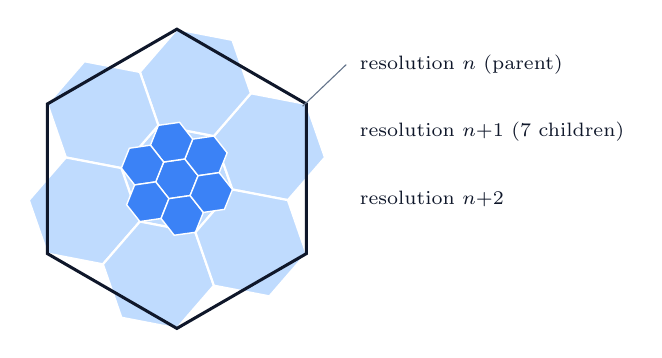
\begin{tikzpicture}
\fill[h3b200, draw=white, line width=0.8pt] (0.470,0.543) -- (-0.235,0.679) -- (-0.705,0.136) -- (-0.470,-0.543) -- (0.235,-0.679) -- (0.705,-0.136) -- cycle;
\fill[h3b200, draw=white, line width=0.8pt] (1.645,0.950) -- (0.940,1.086) -- (0.470,0.543) -- (0.705,-0.136) -- (1.410,-0.271) -- (1.881,0.271) -- cycle;
\fill[h3b200, draw=white, line width=0.8pt] (0.705,1.764) -- (-0.000,1.900) -- (-0.470,1.357) -- (-0.235,0.679) -- (0.470,0.543) -- (0.940,1.086) -- cycle;
\fill[h3b200, draw=white, line width=0.8pt] (-0.470,1.357) -- (-1.175,1.493) -- (-1.645,0.950) -- (-1.410,0.271) -- (-0.705,0.136) -- (-0.235,0.679) -- cycle;
\fill[h3b200, draw=white, line width=0.8pt] (-0.705,0.136) -- (-1.410,0.271) -- (-1.881,-0.271) -- (-1.645,-0.950) -- (-0.940,-1.086) -- (-0.470,-0.543) -- cycle;
\fill[h3b200, draw=white, line width=0.8pt] (0.235,-0.679) -- (-0.470,-0.543) -- (-0.940,-1.086) -- (-0.705,-1.764) -- (-0.000,-1.900) -- (0.470,-1.357) -- cycle;
\fill[h3b200, draw=white, line width=0.8pt] (1.410,-0.271) -- (0.705,-0.136) -- (0.235,-0.679) -- (0.470,-1.357) -- (1.175,-1.493) -- (1.645,-0.950) -- cycle;
\fill[h3b500, draw=white, line width=0.5pt] (0.101,0.252) -- (-0.168,0.213) -- (-0.269,-0.039) -- (-0.101,-0.252) -- (0.168,-0.213) -- (0.269,0.039) -- cycle;
\fill[h3b500, draw=white, line width=0.5pt] (0.470,0.543) -- (0.201,0.504) -- (0.101,0.252) -- (0.269,0.039) -- (0.537,0.078) -- (0.638,0.330) -- cycle;
\fill[h3b500, draw=white, line width=0.5pt] (0.034,0.717) -- (-0.235,0.679) -- (-0.336,0.427) -- (-0.168,0.213) -- (0.101,0.252) -- (0.201,0.504) -- cycle;
\fill[h3b500, draw=white, line width=0.5pt] (-0.336,0.427) -- (-0.604,0.388) -- (-0.705,0.136) -- (-0.537,-0.078) -- (-0.269,-0.039) -- (-0.168,0.213) -- cycle;
\fill[h3b500, draw=white, line width=0.5pt] (-0.269,-0.039) -- (-0.537,-0.078) -- (-0.638,-0.330) -- (-0.470,-0.543) -- (-0.201,-0.504) -- (-0.101,-0.252) -- cycle;
\fill[h3b500, draw=white, line width=0.5pt] (0.168,-0.213) -- (-0.101,-0.252) -- (-0.201,-0.504) -- (-0.034,-0.717) -- (0.235,-0.679) -- (0.336,-0.427) -- cycle;
\fill[h3b500, draw=white, line width=0.5pt] (0.537,0.078) -- (0.269,0.039) -- (0.168,-0.213) -- (0.336,-0.427) -- (0.604,-0.388) -- (0.705,-0.136) -- cycle;
\draw[inkP, line width=1.1pt] (1.645,0.950) -- (0.000,1.900) -- (-1.645,0.950) -- (-1.645,-0.950) -- (-0.000,-1.900) -- (1.645,-0.950) -- cycle;
\node[font=\scriptsize, text=inkP, anchor=west] at (2.2,1.45) {resolution $n$ (parent)};
\draw[inkM, line width=0.4pt] (2.15,1.45) -- (1.596,0.921);
\node[font=\scriptsize, text=inkP, anchor=west] at (2.2,0.6) {resolution $n{+}1$ (7 children)};
\node[font=\scriptsize, text=inkP, anchor=west] at (2.2,-0.25) {resolution $n{+}2$};
\end{tikzpicture}

  \caption{Aperture-7 hierarchical nesting of the H3 grid: each parent cell
    at resolution $n$ subdivides into approximately seven children at
    resolution $n{+}1$; truncating an index string coarsens the view.}
  \label{fig:hierarchy}
\end{figure}

% ============================================================================
\section{The Case Against Administrative Geography}
\label{sec:admin}

Administrative polygons exist to govern, not to measure markets. Used as
analytical units they introduce three distinct, compounding distortions.

\subsection{The Modifiable Areal Unit Problem}

A \emph{desa} in dense urban Jakarta can cover under 1\,km$^2$ and hold
30{,}000 residents; a \emph{desa} in Kalimantan can span hundreds of square
kilometers with fewer than 1{,}000. Any choropleth of revenue, population,
or penetration built on such units is dominated visually and statistically
by polygon \emph{size} rather than by the phenomenon being mapped: vast
sparse districts swamp the map while the urban cores where the business is
actually won or lost vanish into slivers. Figure~\ref{fig:maup} shows the
effect on our study corridor with the underlying data held constant ---
district-level aggregation (panel~a) manufactures large homogeneous
plateaus and erases the demand gradients that the uniform resolution-8
grid (panel~b) preserves. The distortion is not a visualization nuisance;
it propagates into every downstream ratio. Standardizing the archipelago
onto ${\sim}0.737$\,km$^2$ hexagons makes ``revenue per cell'' an
apples-to-apples quantity from Jakarta to Kalimantan.

\subsection{Cross-Border Catchment Blindness}

Consumers do not respect political borders. A store on the western edge of
DKI Jakarta draws naturally from Tangerang in Banten province; a
distribution hub near a provincial boundary serves both sides. Grouping
metrics by \emph{kota} erects artificial walls through these organic
catchments: the store's performance is judged against the population of
the wrong polygon, and the demand it actually serves is credited to a
neighbor. On the spine, a catchment is simply the set of cells within $k$
rings of a location --- a neighborhood query that crosses provincial
borders as indifferently as consumers do
(Section~\ref{sec:method}, Figure~\ref{fig:kring}).

\subsection{\emph{Pemekaran} Instability}

Indonesian administrative geography is a moving target: provinces,
regencies, and villages split (\emph{pemekaran}) with regularity. Each
split breaks the join key of every historical dataset aggregated to the
old boundaries --- year-over-year comparisons must either be abandoned or
rebuilt through error-prone crosswalk tables. H3 cells, by contrast, are
mathematically fixed: the cell containing a given coordinate at a given
resolution is the same today, a decade ago, and a decade hence. A spine
keyed to H3 makes the organization's spatial history immune to political
redistricting by construction.

\begin{figure*}[t]
  \centering
  % Auto-generated by generate_figures.py -- do not edit by hand
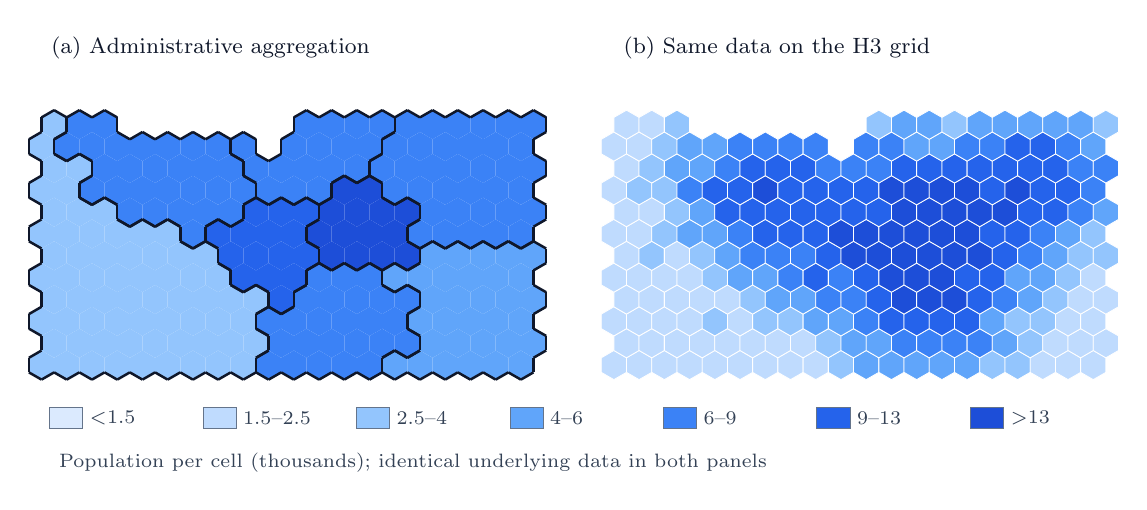
\begin{tikzpicture}
\begin{scope}
\fill[h3b300] (0.160,0.092) -- (0.000,0.185) -- (-0.160,0.092) -- (-0.160,-0.093) -- (-0.000,-0.185) -- (0.160,-0.093) -- cycle;
\fill[h3b300] (0.481,0.092) -- (0.320,0.185) -- (0.160,0.092) -- (0.160,-0.093) -- (0.320,-0.185) -- (0.481,-0.093) -- cycle;
\fill[h3b300] (0.801,0.092) -- (0.641,0.185) -- (0.481,0.092) -- (0.481,-0.093) -- (0.641,-0.185) -- (0.801,-0.093) -- cycle;
\fill[h3b300] (1.122,0.092) -- (0.961,0.185) -- (0.801,0.092) -- (0.801,-0.093) -- (0.961,-0.185) -- (1.122,-0.093) -- cycle;
\fill[h3b300] (1.442,0.092) -- (1.282,0.185) -- (1.122,0.092) -- (1.122,-0.093) -- (1.282,-0.185) -- (1.442,-0.093) -- cycle;
\fill[h3b300] (1.762,0.092) -- (1.602,0.185) -- (1.442,0.092) -- (1.442,-0.093) -- (1.602,-0.185) -- (1.762,-0.093) -- cycle;
\fill[h3b300] (2.083,0.092) -- (1.923,0.185) -- (1.762,0.092) -- (1.762,-0.093) -- (1.923,-0.185) -- (2.083,-0.093) -- cycle;
\fill[h3b300] (2.403,0.092) -- (2.243,0.185) -- (2.083,0.092) -- (2.083,-0.093) -- (2.243,-0.185) -- (2.403,-0.093) -- cycle;
\fill[h3b300] (2.724,0.092) -- (2.563,0.185) -- (2.403,0.092) -- (2.403,-0.093) -- (2.563,-0.185) -- (2.724,-0.093) -- cycle;
\fill[h3b500] (3.044,0.092) -- (2.884,0.185) -- (2.724,0.092) -- (2.724,-0.093) -- (2.884,-0.185) -- (3.044,-0.093) -- cycle;
\fill[h3b500] (3.365,0.092) -- (3.204,0.185) -- (3.044,0.092) -- (3.044,-0.093) -- (3.204,-0.185) -- (3.365,-0.093) -- cycle;
\fill[h3b500] (3.685,0.092) -- (3.525,0.185) -- (3.365,0.092) -- (3.365,-0.093) -- (3.525,-0.185) -- (3.685,-0.093) -- cycle;
\fill[h3b500] (4.005,0.092) -- (3.845,0.185) -- (3.685,0.092) -- (3.685,-0.093) -- (3.845,-0.185) -- (4.005,-0.093) -- cycle;
\fill[h3b500] (4.326,0.092) -- (4.166,0.185) -- (4.005,0.092) -- (4.005,-0.093) -- (4.166,-0.185) -- (4.326,-0.093) -- cycle;
\fill[h3b400] (4.646,0.092) -- (4.486,0.185) -- (4.326,0.092) -- (4.326,-0.093) -- (4.486,-0.185) -- (4.646,-0.093) -- cycle;
\fill[h3b400] (4.967,0.092) -- (4.806,0.185) -- (4.646,0.092) -- (4.646,-0.093) -- (4.806,-0.185) -- (4.967,-0.093) -- cycle;
\fill[h3b400] (5.287,0.092) -- (5.127,0.185) -- (4.967,0.092) -- (4.967,-0.093) -- (5.127,-0.185) -- (5.287,-0.093) -- cycle;
\fill[h3b400] (5.608,0.092) -- (5.447,0.185) -- (5.287,0.092) -- (5.287,-0.093) -- (5.447,-0.185) -- (5.608,-0.093) -- cycle;
\fill[h3b400] (5.928,0.092) -- (5.768,0.185) -- (5.608,0.092) -- (5.608,-0.093) -- (5.768,-0.185) -- (5.928,-0.093) -- cycle;
\fill[h3b400] (6.248,0.092) -- (6.088,0.185) -- (5.928,0.092) -- (5.928,-0.093) -- (6.088,-0.185) -- (6.248,-0.093) -- cycle;
\fill[h3b300] (0.320,0.370) -- (0.160,0.462) -- (-0.000,0.370) -- (0.000,0.185) -- (0.160,0.092) -- (0.320,0.185) -- cycle;
\fill[h3b300] (0.641,0.370) -- (0.481,0.462) -- (0.320,0.370) -- (0.320,0.185) -- (0.481,0.092) -- (0.641,0.185) -- cycle;
\fill[h3b300] (0.961,0.370) -- (0.801,0.462) -- (0.641,0.370) -- (0.641,0.185) -- (0.801,0.092) -- (0.961,0.185) -- cycle;
\fill[h3b300] (1.282,0.370) -- (1.122,0.462) -- (0.961,0.370) -- (0.961,0.185) -- (1.122,0.092) -- (1.282,0.185) -- cycle;
\fill[h3b300] (1.602,0.370) -- (1.442,0.462) -- (1.282,0.370) -- (1.282,0.185) -- (1.442,0.092) -- (1.602,0.185) -- cycle;
\fill[h3b300] (1.923,0.370) -- (1.762,0.462) -- (1.602,0.370) -- (1.602,0.185) -- (1.762,0.092) -- (1.923,0.185) -- cycle;
\fill[h3b300] (2.243,0.370) -- (2.083,0.462) -- (1.923,0.370) -- (1.923,0.185) -- (2.083,0.092) -- (2.243,0.185) -- cycle;
\fill[h3b300] (2.563,0.370) -- (2.403,0.462) -- (2.243,0.370) -- (2.243,0.185) -- (2.403,0.092) -- (2.563,0.185) -- cycle;
\fill[h3b300] (2.884,0.370) -- (2.724,0.462) -- (2.563,0.370) -- (2.563,0.185) -- (2.724,0.092) -- (2.884,0.185) -- cycle;
\fill[h3b500] (3.204,0.370) -- (3.044,0.462) -- (2.884,0.370) -- (2.884,0.185) -- (3.044,0.092) -- (3.204,0.185) -- cycle;
\fill[h3b500] (3.525,0.370) -- (3.365,0.462) -- (3.204,0.370) -- (3.204,0.185) -- (3.365,0.092) -- (3.525,0.185) -- cycle;
\fill[h3b500] (3.845,0.370) -- (3.685,0.462) -- (3.525,0.370) -- (3.525,0.185) -- (3.685,0.092) -- (3.845,0.185) -- cycle;
\fill[h3b500] (4.166,0.370) -- (4.005,0.462) -- (3.845,0.370) -- (3.845,0.185) -- (4.005,0.092) -- (4.166,0.185) -- cycle;
\fill[h3b500] (4.486,0.370) -- (4.326,0.462) -- (4.166,0.370) -- (4.166,0.185) -- (4.326,0.092) -- (4.486,0.185) -- cycle;
\fill[h3b500] (4.806,0.370) -- (4.646,0.462) -- (4.486,0.370) -- (4.486,0.185) -- (4.646,0.092) -- (4.806,0.185) -- cycle;
\fill[h3b400] (5.127,0.370) -- (4.967,0.462) -- (4.806,0.370) -- (4.806,0.185) -- (4.967,0.092) -- (5.127,0.185) -- cycle;
\fill[h3b400] (5.447,0.370) -- (5.287,0.462) -- (5.127,0.370) -- (5.127,0.185) -- (5.287,0.092) -- (5.447,0.185) -- cycle;
\fill[h3b400] (5.768,0.370) -- (5.608,0.462) -- (5.447,0.370) -- (5.447,0.185) -- (5.608,0.092) -- (5.768,0.185) -- cycle;
\fill[h3b400] (6.088,0.370) -- (5.928,0.462) -- (5.768,0.370) -- (5.768,0.185) -- (5.928,0.092) -- (6.088,0.185) -- cycle;
\fill[h3b400] (6.409,0.370) -- (6.248,0.462) -- (6.088,0.370) -- (6.088,0.185) -- (6.248,0.092) -- (6.409,0.185) -- cycle;
\fill[h3b300] (0.160,0.647) -- (0.000,0.740) -- (-0.160,0.647) -- (-0.160,0.462) -- (-0.000,0.370) -- (0.160,0.462) -- cycle;
\fill[h3b300] (0.481,0.647) -- (0.320,0.740) -- (0.160,0.647) -- (0.160,0.462) -- (0.320,0.370) -- (0.481,0.462) -- cycle;
\fill[h3b300] (0.801,0.647) -- (0.641,0.740) -- (0.481,0.647) -- (0.481,0.462) -- (0.641,0.370) -- (0.801,0.462) -- cycle;
\fill[h3b300] (1.122,0.647) -- (0.961,0.740) -- (0.801,0.647) -- (0.801,0.462) -- (0.961,0.370) -- (1.122,0.462) -- cycle;
\fill[h3b300] (1.442,0.647) -- (1.282,0.740) -- (1.122,0.647) -- (1.122,0.462) -- (1.282,0.370) -- (1.442,0.462) -- cycle;
\fill[h3b300] (1.762,0.647) -- (1.602,0.740) -- (1.442,0.647) -- (1.442,0.462) -- (1.602,0.370) -- (1.762,0.462) -- cycle;
\fill[h3b300] (2.083,0.647) -- (1.923,0.740) -- (1.762,0.647) -- (1.762,0.462) -- (1.923,0.370) -- (2.083,0.462) -- cycle;
\fill[h3b300] (2.403,0.647) -- (2.243,0.740) -- (2.083,0.647) -- (2.083,0.462) -- (2.243,0.370) -- (2.403,0.462) -- cycle;
\fill[h3b300] (2.724,0.647) -- (2.563,0.740) -- (2.403,0.647) -- (2.403,0.462) -- (2.563,0.370) -- (2.724,0.462) -- cycle;
\fill[h3b500] (3.044,0.647) -- (2.884,0.740) -- (2.724,0.647) -- (2.724,0.462) -- (2.884,0.370) -- (3.044,0.462) -- cycle;
\fill[h3b500] (3.365,0.647) -- (3.204,0.740) -- (3.044,0.647) -- (3.044,0.462) -- (3.204,0.370) -- (3.365,0.462) -- cycle;
\fill[h3b500] (3.685,0.647) -- (3.525,0.740) -- (3.365,0.647) -- (3.365,0.462) -- (3.525,0.370) -- (3.685,0.462) -- cycle;
\fill[h3b500] (4.005,0.647) -- (3.845,0.740) -- (3.685,0.647) -- (3.685,0.462) -- (3.845,0.370) -- (4.005,0.462) -- cycle;
\fill[h3b500] (4.326,0.647) -- (4.166,0.740) -- (4.005,0.647) -- (4.005,0.462) -- (4.166,0.370) -- (4.326,0.462) -- cycle;
\fill[h3b500] (4.646,0.647) -- (4.486,0.740) -- (4.326,0.647) -- (4.326,0.462) -- (4.486,0.370) -- (4.646,0.462) -- cycle;
\fill[h3b400] (4.967,0.647) -- (4.806,0.740) -- (4.646,0.647) -- (4.646,0.462) -- (4.806,0.370) -- (4.967,0.462) -- cycle;
\fill[h3b400] (5.287,0.647) -- (5.127,0.740) -- (4.967,0.647) -- (4.967,0.462) -- (5.127,0.370) -- (5.287,0.462) -- cycle;
\fill[h3b400] (5.608,0.647) -- (5.447,0.740) -- (5.287,0.647) -- (5.287,0.462) -- (5.447,0.370) -- (5.608,0.462) -- cycle;
\fill[h3b400] (5.928,0.647) -- (5.768,0.740) -- (5.608,0.647) -- (5.608,0.462) -- (5.768,0.370) -- (5.928,0.462) -- cycle;
\fill[h3b400] (6.248,0.647) -- (6.088,0.740) -- (5.928,0.647) -- (5.928,0.462) -- (6.088,0.370) -- (6.248,0.462) -- cycle;
\fill[h3b300] (0.320,0.925) -- (0.160,1.017) -- (-0.000,0.925) -- (0.000,0.740) -- (0.160,0.647) -- (0.320,0.740) -- cycle;
\fill[h3b300] (0.641,0.925) -- (0.481,1.017) -- (0.320,0.925) -- (0.320,0.740) -- (0.481,0.647) -- (0.641,0.740) -- cycle;
\fill[h3b300] (0.961,0.925) -- (0.801,1.017) -- (0.641,0.925) -- (0.641,0.740) -- (0.801,0.647) -- (0.961,0.740) -- cycle;
\fill[h3b300] (1.282,0.925) -- (1.122,1.017) -- (0.961,0.925) -- (0.961,0.740) -- (1.122,0.647) -- (1.282,0.740) -- cycle;
\fill[h3b300] (1.602,0.925) -- (1.442,1.017) -- (1.282,0.925) -- (1.282,0.740) -- (1.442,0.647) -- (1.602,0.740) -- cycle;
\fill[h3b300] (1.923,0.925) -- (1.762,1.017) -- (1.602,0.925) -- (1.602,0.740) -- (1.762,0.647) -- (1.923,0.740) -- cycle;
\fill[h3b300] (2.243,0.925) -- (2.083,1.017) -- (1.923,0.925) -- (1.923,0.740) -- (2.083,0.647) -- (2.243,0.740) -- cycle;
\fill[h3b300] (2.563,0.925) -- (2.403,1.017) -- (2.243,0.925) -- (2.243,0.740) -- (2.403,0.647) -- (2.563,0.740) -- cycle;
\fill[h3b300] (2.884,0.925) -- (2.724,1.017) -- (2.563,0.925) -- (2.563,0.740) -- (2.724,0.647) -- (2.884,0.740) -- cycle;
\fill[h3b600] (3.204,0.925) -- (3.044,1.017) -- (2.884,0.925) -- (2.884,0.740) -- (3.044,0.647) -- (3.204,0.740) -- cycle;
\fill[h3b500] (3.525,0.925) -- (3.365,1.017) -- (3.204,0.925) -- (3.204,0.740) -- (3.365,0.647) -- (3.525,0.740) -- cycle;
\fill[h3b500] (3.845,0.925) -- (3.685,1.017) -- (3.525,0.925) -- (3.525,0.740) -- (3.685,0.647) -- (3.845,0.740) -- cycle;
\fill[h3b500] (4.166,0.925) -- (4.005,1.017) -- (3.845,0.925) -- (3.845,0.740) -- (4.005,0.647) -- (4.166,0.740) -- cycle;
\fill[h3b500] (4.486,0.925) -- (4.326,1.017) -- (4.166,0.925) -- (4.166,0.740) -- (4.326,0.647) -- (4.486,0.740) -- cycle;
\fill[h3b500] (4.806,0.925) -- (4.646,1.017) -- (4.486,0.925) -- (4.486,0.740) -- (4.646,0.647) -- (4.806,0.740) -- cycle;
\fill[h3b400] (5.127,0.925) -- (4.967,1.017) -- (4.806,0.925) -- (4.806,0.740) -- (4.967,0.647) -- (5.127,0.740) -- cycle;
\fill[h3b400] (5.447,0.925) -- (5.287,1.017) -- (5.127,0.925) -- (5.127,0.740) -- (5.287,0.647) -- (5.447,0.740) -- cycle;
\fill[h3b400] (5.768,0.925) -- (5.608,1.017) -- (5.447,0.925) -- (5.447,0.740) -- (5.608,0.647) -- (5.768,0.740) -- cycle;
\fill[h3b400] (6.088,0.925) -- (5.928,1.017) -- (5.768,0.925) -- (5.768,0.740) -- (5.928,0.647) -- (6.088,0.740) -- cycle;
\fill[h3b400] (6.409,0.925) -- (6.248,1.017) -- (6.088,0.925) -- (6.088,0.740) -- (6.248,0.647) -- (6.409,0.740) -- cycle;
\fill[h3b300] (0.160,1.202) -- (0.000,1.295) -- (-0.160,1.202) -- (-0.160,1.017) -- (-0.000,0.925) -- (0.160,1.017) -- cycle;
\fill[h3b300] (0.481,1.202) -- (0.320,1.295) -- (0.160,1.202) -- (0.160,1.017) -- (0.320,0.925) -- (0.481,1.017) -- cycle;
\fill[h3b300] (0.801,1.202) -- (0.641,1.295) -- (0.481,1.202) -- (0.481,1.017) -- (0.641,0.925) -- (0.801,1.017) -- cycle;
\fill[h3b300] (1.122,1.202) -- (0.961,1.295) -- (0.801,1.202) -- (0.801,1.017) -- (0.961,0.925) -- (1.122,1.017) -- cycle;
\fill[h3b300] (1.442,1.202) -- (1.282,1.295) -- (1.122,1.202) -- (1.122,1.017) -- (1.282,0.925) -- (1.442,1.017) -- cycle;
\fill[h3b300] (1.762,1.202) -- (1.602,1.295) -- (1.442,1.202) -- (1.442,1.017) -- (1.602,0.925) -- (1.762,1.017) -- cycle;
\fill[h3b300] (2.083,1.202) -- (1.923,1.295) -- (1.762,1.202) -- (1.762,1.017) -- (1.923,0.925) -- (2.083,1.017) -- cycle;
\fill[h3b300] (2.403,1.202) -- (2.243,1.295) -- (2.083,1.202) -- (2.083,1.017) -- (2.243,0.925) -- (2.403,1.017) -- cycle;
\fill[h3b600] (2.724,1.202) -- (2.563,1.295) -- (2.403,1.202) -- (2.403,1.017) -- (2.563,0.925) -- (2.724,1.017) -- cycle;
\fill[h3b600] (3.044,1.202) -- (2.884,1.295) -- (2.724,1.202) -- (2.724,1.017) -- (2.884,0.925) -- (3.044,1.017) -- cycle;
\fill[h3b600] (3.365,1.202) -- (3.204,1.295) -- (3.044,1.202) -- (3.044,1.017) -- (3.204,0.925) -- (3.365,1.017) -- cycle;
\fill[h3b500] (3.685,1.202) -- (3.525,1.295) -- (3.365,1.202) -- (3.365,1.017) -- (3.525,0.925) -- (3.685,1.017) -- cycle;
\fill[h3b500] (4.005,1.202) -- (3.845,1.295) -- (3.685,1.202) -- (3.685,1.017) -- (3.845,0.925) -- (4.005,1.017) -- cycle;
\fill[h3b500] (4.326,1.202) -- (4.166,1.295) -- (4.005,1.202) -- (4.005,1.017) -- (4.166,0.925) -- (4.326,1.017) -- cycle;
\fill[h3b400] (4.646,1.202) -- (4.486,1.295) -- (4.326,1.202) -- (4.326,1.017) -- (4.486,0.925) -- (4.646,1.017) -- cycle;
\fill[h3b400] (4.967,1.202) -- (4.806,1.295) -- (4.646,1.202) -- (4.646,1.017) -- (4.806,0.925) -- (4.967,1.017) -- cycle;
\fill[h3b400] (5.287,1.202) -- (5.127,1.295) -- (4.967,1.202) -- (4.967,1.017) -- (5.127,0.925) -- (5.287,1.017) -- cycle;
\fill[h3b400] (5.608,1.202) -- (5.447,1.295) -- (5.287,1.202) -- (5.287,1.017) -- (5.447,0.925) -- (5.608,1.017) -- cycle;
\fill[h3b400] (5.928,1.202) -- (5.768,1.295) -- (5.608,1.202) -- (5.608,1.017) -- (5.768,0.925) -- (5.928,1.017) -- cycle;
\fill[h3b400] (6.248,1.202) -- (6.088,1.295) -- (5.928,1.202) -- (5.928,1.017) -- (6.088,0.925) -- (6.248,1.017) -- cycle;
\fill[h3b300] (0.320,1.480) -- (0.160,1.572) -- (-0.000,1.480) -- (0.000,1.295) -- (0.160,1.202) -- (0.320,1.295) -- cycle;
\fill[h3b300] (0.641,1.480) -- (0.481,1.572) -- (0.320,1.480) -- (0.320,1.295) -- (0.481,1.202) -- (0.641,1.295) -- cycle;
\fill[h3b300] (0.961,1.480) -- (0.801,1.572) -- (0.641,1.480) -- (0.641,1.295) -- (0.801,1.202) -- (0.961,1.295) -- cycle;
\fill[h3b300] (1.282,1.480) -- (1.122,1.572) -- (0.961,1.480) -- (0.961,1.295) -- (1.122,1.202) -- (1.282,1.295) -- cycle;
\fill[h3b300] (1.602,1.480) -- (1.442,1.572) -- (1.282,1.480) -- (1.282,1.295) -- (1.442,1.202) -- (1.602,1.295) -- cycle;
\fill[h3b300] (1.923,1.480) -- (1.762,1.572) -- (1.602,1.480) -- (1.602,1.295) -- (1.762,1.202) -- (1.923,1.295) -- cycle;
\fill[h3b300] (2.243,1.480) -- (2.083,1.572) -- (1.923,1.480) -- (1.923,1.295) -- (2.083,1.202) -- (2.243,1.295) -- cycle;
\fill[h3b600] (2.563,1.480) -- (2.403,1.572) -- (2.243,1.480) -- (2.243,1.295) -- (2.403,1.202) -- (2.563,1.295) -- cycle;
\fill[h3b600] (2.884,1.480) -- (2.724,1.572) -- (2.563,1.480) -- (2.563,1.295) -- (2.724,1.202) -- (2.884,1.295) -- cycle;
\fill[h3b600] (3.204,1.480) -- (3.044,1.572) -- (2.884,1.480) -- (2.884,1.295) -- (3.044,1.202) -- (3.204,1.295) -- cycle;
\fill[h3b600] (3.525,1.480) -- (3.365,1.572) -- (3.204,1.480) -- (3.204,1.295) -- (3.365,1.202) -- (3.525,1.295) -- cycle;
\fill[h3b700] (3.845,1.480) -- (3.685,1.572) -- (3.525,1.480) -- (3.525,1.295) -- (3.685,1.202) -- (3.845,1.295) -- cycle;
\fill[h3b700] (4.166,1.480) -- (4.005,1.572) -- (3.845,1.480) -- (3.845,1.295) -- (4.005,1.202) -- (4.166,1.295) -- cycle;
\fill[h3b700] (4.486,1.480) -- (4.326,1.572) -- (4.166,1.480) -- (4.166,1.295) -- (4.326,1.202) -- (4.486,1.295) -- cycle;
\fill[h3b700] (4.806,1.480) -- (4.646,1.572) -- (4.486,1.480) -- (4.486,1.295) -- (4.646,1.202) -- (4.806,1.295) -- cycle;
\fill[h3b400] (5.127,1.480) -- (4.967,1.572) -- (4.806,1.480) -- (4.806,1.295) -- (4.967,1.202) -- (5.127,1.295) -- cycle;
\fill[h3b400] (5.447,1.480) -- (5.287,1.572) -- (5.127,1.480) -- (5.127,1.295) -- (5.287,1.202) -- (5.447,1.295) -- cycle;
\fill[h3b400] (5.768,1.480) -- (5.608,1.572) -- (5.447,1.480) -- (5.447,1.295) -- (5.608,1.202) -- (5.768,1.295) -- cycle;
\fill[h3b400] (6.088,1.480) -- (5.928,1.572) -- (5.768,1.480) -- (5.768,1.295) -- (5.928,1.202) -- (6.088,1.295) -- cycle;
\fill[h3b400] (6.409,1.480) -- (6.248,1.572) -- (6.088,1.480) -- (6.088,1.295) -- (6.248,1.202) -- (6.409,1.295) -- cycle;
\fill[h3b300] (0.160,1.757) -- (0.000,1.850) -- (-0.160,1.757) -- (-0.160,1.572) -- (-0.000,1.480) -- (0.160,1.572) -- cycle;
\fill[h3b300] (0.481,1.757) -- (0.320,1.850) -- (0.160,1.757) -- (0.160,1.572) -- (0.320,1.480) -- (0.481,1.572) -- cycle;
\fill[h3b300] (0.801,1.757) -- (0.641,1.850) -- (0.481,1.757) -- (0.481,1.572) -- (0.641,1.480) -- (0.801,1.572) -- cycle;
\fill[h3b300] (1.122,1.757) -- (0.961,1.850) -- (0.801,1.757) -- (0.801,1.572) -- (0.961,1.480) -- (1.122,1.572) -- cycle;
\fill[h3b300] (1.442,1.757) -- (1.282,1.850) -- (1.122,1.757) -- (1.122,1.572) -- (1.282,1.480) -- (1.442,1.572) -- cycle;
\fill[h3b300] (1.762,1.757) -- (1.602,1.850) -- (1.442,1.757) -- (1.442,1.572) -- (1.602,1.480) -- (1.762,1.572) -- cycle;
\fill[h3b500] (2.083,1.757) -- (1.923,1.850) -- (1.762,1.757) -- (1.762,1.572) -- (1.923,1.480) -- (2.083,1.572) -- cycle;
\fill[h3b600] (2.403,1.757) -- (2.243,1.850) -- (2.083,1.757) -- (2.083,1.572) -- (2.243,1.480) -- (2.403,1.572) -- cycle;
\fill[h3b600] (2.724,1.757) -- (2.563,1.850) -- (2.403,1.757) -- (2.403,1.572) -- (2.563,1.480) -- (2.724,1.572) -- cycle;
\fill[h3b600] (3.044,1.757) -- (2.884,1.850) -- (2.724,1.757) -- (2.724,1.572) -- (2.884,1.480) -- (3.044,1.572) -- cycle;
\fill[h3b600] (3.365,1.757) -- (3.204,1.850) -- (3.044,1.757) -- (3.044,1.572) -- (3.204,1.480) -- (3.365,1.572) -- cycle;
\fill[h3b700] (3.685,1.757) -- (3.525,1.850) -- (3.365,1.757) -- (3.365,1.572) -- (3.525,1.480) -- (3.685,1.572) -- cycle;
\fill[h3b700] (4.005,1.757) -- (3.845,1.850) -- (3.685,1.757) -- (3.685,1.572) -- (3.845,1.480) -- (4.005,1.572) -- cycle;
\fill[h3b700] (4.326,1.757) -- (4.166,1.850) -- (4.005,1.757) -- (4.005,1.572) -- (4.166,1.480) -- (4.326,1.572) -- cycle;
\fill[h3b700] (4.646,1.757) -- (4.486,1.850) -- (4.326,1.757) -- (4.326,1.572) -- (4.486,1.480) -- (4.646,1.572) -- cycle;
\fill[h3b500] (4.967,1.757) -- (4.806,1.850) -- (4.646,1.757) -- (4.646,1.572) -- (4.806,1.480) -- (4.967,1.572) -- cycle;
\fill[h3b500] (5.287,1.757) -- (5.127,1.850) -- (4.967,1.757) -- (4.967,1.572) -- (5.127,1.480) -- (5.287,1.572) -- cycle;
\fill[h3b500] (5.608,1.757) -- (5.447,1.850) -- (5.287,1.757) -- (5.287,1.572) -- (5.447,1.480) -- (5.608,1.572) -- cycle;
\fill[h3b500] (5.928,1.757) -- (5.768,1.850) -- (5.608,1.757) -- (5.608,1.572) -- (5.768,1.480) -- (5.928,1.572) -- cycle;
\fill[h3b500] (6.248,1.757) -- (6.088,1.850) -- (5.928,1.757) -- (5.928,1.572) -- (6.088,1.480) -- (6.248,1.572) -- cycle;
\fill[h3b300] (0.320,2.035) -- (0.160,2.127) -- (-0.000,2.035) -- (0.000,1.850) -- (0.160,1.757) -- (0.320,1.850) -- cycle;
\fill[h3b300] (0.641,2.035) -- (0.481,2.127) -- (0.320,2.035) -- (0.320,1.850) -- (0.481,1.757) -- (0.641,1.850) -- cycle;
\fill[h3b300] (0.961,2.035) -- (0.801,2.127) -- (0.641,2.035) -- (0.641,1.850) -- (0.801,1.757) -- (0.961,1.850) -- cycle;
\fill[h3b500] (1.282,2.035) -- (1.122,2.127) -- (0.961,2.035) -- (0.961,1.850) -- (1.122,1.757) -- (1.282,1.850) -- cycle;
\fill[h3b500] (1.602,2.035) -- (1.442,2.127) -- (1.282,2.035) -- (1.282,1.850) -- (1.442,1.757) -- (1.602,1.850) -- cycle;
\fill[h3b500] (1.923,2.035) -- (1.762,2.127) -- (1.602,2.035) -- (1.602,1.850) -- (1.762,1.757) -- (1.923,1.850) -- cycle;
\fill[h3b500] (2.243,2.035) -- (2.083,2.127) -- (1.923,2.035) -- (1.923,1.850) -- (2.083,1.757) -- (2.243,1.850) -- cycle;
\fill[h3b500] (2.563,2.035) -- (2.403,2.127) -- (2.243,2.035) -- (2.243,1.850) -- (2.403,1.757) -- (2.563,1.850) -- cycle;
\fill[h3b600] (2.884,2.035) -- (2.724,2.127) -- (2.563,2.035) -- (2.563,1.850) -- (2.724,1.757) -- (2.884,1.850) -- cycle;
\fill[h3b600] (3.204,2.035) -- (3.044,2.127) -- (2.884,2.035) -- (2.884,1.850) -- (3.044,1.757) -- (3.204,1.850) -- cycle;
\fill[h3b600] (3.525,2.035) -- (3.365,2.127) -- (3.204,2.035) -- (3.204,1.850) -- (3.365,1.757) -- (3.525,1.850) -- cycle;
\fill[h3b700] (3.845,2.035) -- (3.685,2.127) -- (3.525,2.035) -- (3.525,1.850) -- (3.685,1.757) -- (3.845,1.850) -- cycle;
\fill[h3b700] (4.166,2.035) -- (4.005,2.127) -- (3.845,2.035) -- (3.845,1.850) -- (4.005,1.757) -- (4.166,1.850) -- cycle;
\fill[h3b700] (4.486,2.035) -- (4.326,2.127) -- (4.166,2.035) -- (4.166,1.850) -- (4.326,1.757) -- (4.486,1.850) -- cycle;
\fill[h3b700] (4.806,2.035) -- (4.646,2.127) -- (4.486,2.035) -- (4.486,1.850) -- (4.646,1.757) -- (4.806,1.850) -- cycle;
\fill[h3b500] (5.127,2.035) -- (4.967,2.127) -- (4.806,2.035) -- (4.806,1.850) -- (4.967,1.757) -- (5.127,1.850) -- cycle;
\fill[h3b500] (5.447,2.035) -- (5.287,2.127) -- (5.127,2.035) -- (5.127,1.850) -- (5.287,1.757) -- (5.447,1.850) -- cycle;
\fill[h3b500] (5.768,2.035) -- (5.608,2.127) -- (5.447,2.035) -- (5.447,1.850) -- (5.608,1.757) -- (5.768,1.850) -- cycle;
\fill[h3b500] (6.088,2.035) -- (5.928,2.127) -- (5.768,2.035) -- (5.768,1.850) -- (5.928,1.757) -- (6.088,1.850) -- cycle;
\fill[h3b500] (6.409,2.035) -- (6.248,2.127) -- (6.088,2.035) -- (6.088,1.850) -- (6.248,1.757) -- (6.409,1.850) -- cycle;
\fill[h3b300] (0.160,2.312) -- (0.000,2.405) -- (-0.160,2.312) -- (-0.160,2.127) -- (-0.000,2.035) -- (0.160,2.127) -- cycle;
\fill[h3b300] (0.481,2.312) -- (0.320,2.405) -- (0.160,2.312) -- (0.160,2.127) -- (0.320,2.035) -- (0.481,2.127) -- cycle;
\fill[h3b500] (0.801,2.312) -- (0.641,2.405) -- (0.481,2.312) -- (0.481,2.127) -- (0.641,2.035) -- (0.801,2.127) -- cycle;
\fill[h3b500] (1.122,2.312) -- (0.961,2.405) -- (0.801,2.312) -- (0.801,2.127) -- (0.961,2.035) -- (1.122,2.127) -- cycle;
\fill[h3b500] (1.442,2.312) -- (1.282,2.405) -- (1.122,2.312) -- (1.122,2.127) -- (1.282,2.035) -- (1.442,2.127) -- cycle;
\fill[h3b500] (1.762,2.312) -- (1.602,2.405) -- (1.442,2.312) -- (1.442,2.127) -- (1.602,2.035) -- (1.762,2.127) -- cycle;
\fill[h3b500] (2.083,2.312) -- (1.923,2.405) -- (1.762,2.312) -- (1.762,2.127) -- (1.923,2.035) -- (2.083,2.127) -- cycle;
\fill[h3b500] (2.403,2.312) -- (2.243,2.405) -- (2.083,2.312) -- (2.083,2.127) -- (2.243,2.035) -- (2.403,2.127) -- cycle;
\fill[h3b500] (2.724,2.312) -- (2.563,2.405) -- (2.403,2.312) -- (2.403,2.127) -- (2.563,2.035) -- (2.724,2.127) -- cycle;
\fill[h3b500] (3.044,2.312) -- (2.884,2.405) -- (2.724,2.312) -- (2.724,2.127) -- (2.884,2.035) -- (3.044,2.127) -- cycle;
\fill[h3b500] (3.365,2.312) -- (3.204,2.405) -- (3.044,2.312) -- (3.044,2.127) -- (3.204,2.035) -- (3.365,2.127) -- cycle;
\fill[h3b500] (3.685,2.312) -- (3.525,2.405) -- (3.365,2.312) -- (3.365,2.127) -- (3.525,2.035) -- (3.685,2.127) -- cycle;
\fill[h3b700] (4.005,2.312) -- (3.845,2.405) -- (3.685,2.312) -- (3.685,2.127) -- (3.845,2.035) -- (4.005,2.127) -- cycle;
\fill[h3b700] (4.326,2.312) -- (4.166,2.405) -- (4.005,2.312) -- (4.005,2.127) -- (4.166,2.035) -- (4.326,2.127) -- cycle;
\fill[h3b500] (4.646,2.312) -- (4.486,2.405) -- (4.326,2.312) -- (4.326,2.127) -- (4.486,2.035) -- (4.646,2.127) -- cycle;
\fill[h3b500] (4.967,2.312) -- (4.806,2.405) -- (4.646,2.312) -- (4.646,2.127) -- (4.806,2.035) -- (4.967,2.127) -- cycle;
\fill[h3b500] (5.287,2.312) -- (5.127,2.405) -- (4.967,2.312) -- (4.967,2.127) -- (5.127,2.035) -- (5.287,2.127) -- cycle;
\fill[h3b500] (5.608,2.312) -- (5.447,2.405) -- (5.287,2.312) -- (5.287,2.127) -- (5.447,2.035) -- (5.608,2.127) -- cycle;
\fill[h3b500] (5.928,2.312) -- (5.768,2.405) -- (5.608,2.312) -- (5.608,2.127) -- (5.768,2.035) -- (5.928,2.127) -- cycle;
\fill[h3b500] (6.248,2.312) -- (6.088,2.405) -- (5.928,2.312) -- (5.928,2.127) -- (6.088,2.035) -- (6.248,2.127) -- cycle;
\fill[h3b300] (0.320,2.590) -- (0.160,2.682) -- (-0.000,2.590) -- (0.000,2.405) -- (0.160,2.312) -- (0.320,2.405) -- cycle;
\fill[h3b300] (0.641,2.590) -- (0.481,2.682) -- (0.320,2.590) -- (0.320,2.405) -- (0.481,2.312) -- (0.641,2.405) -- cycle;
\fill[h3b500] (0.961,2.590) -- (0.801,2.682) -- (0.641,2.590) -- (0.641,2.405) -- (0.801,2.312) -- (0.961,2.405) -- cycle;
\fill[h3b500] (1.282,2.590) -- (1.122,2.682) -- (0.961,2.590) -- (0.961,2.405) -- (1.122,2.312) -- (1.282,2.405) -- cycle;
\fill[h3b500] (1.602,2.590) -- (1.442,2.682) -- (1.282,2.590) -- (1.282,2.405) -- (1.442,2.312) -- (1.602,2.405) -- cycle;
\fill[h3b500] (1.923,2.590) -- (1.762,2.682) -- (1.602,2.590) -- (1.602,2.405) -- (1.762,2.312) -- (1.923,2.405) -- cycle;
\fill[h3b500] (2.243,2.590) -- (2.083,2.682) -- (1.923,2.590) -- (1.923,2.405) -- (2.083,2.312) -- (2.243,2.405) -- cycle;
\fill[h3b500] (2.563,2.590) -- (2.403,2.682) -- (2.243,2.590) -- (2.243,2.405) -- (2.403,2.312) -- (2.563,2.405) -- cycle;
\fill[h3b500] (2.884,2.590) -- (2.724,2.682) -- (2.563,2.590) -- (2.563,2.405) -- (2.724,2.312) -- (2.884,2.405) -- cycle;
\fill[h3b500] (3.204,2.590) -- (3.044,2.682) -- (2.884,2.590) -- (2.884,2.405) -- (3.044,2.312) -- (3.204,2.405) -- cycle;
\fill[h3b500] (3.525,2.590) -- (3.365,2.682) -- (3.204,2.590) -- (3.204,2.405) -- (3.365,2.312) -- (3.525,2.405) -- cycle;
\fill[h3b500] (3.845,2.590) -- (3.685,2.682) -- (3.525,2.590) -- (3.525,2.405) -- (3.685,2.312) -- (3.845,2.405) -- cycle;
\fill[h3b500] (4.166,2.590) -- (4.005,2.682) -- (3.845,2.590) -- (3.845,2.405) -- (4.005,2.312) -- (4.166,2.405) -- cycle;
\fill[h3b500] (4.486,2.590) -- (4.326,2.682) -- (4.166,2.590) -- (4.166,2.405) -- (4.326,2.312) -- (4.486,2.405) -- cycle;
\fill[h3b500] (4.806,2.590) -- (4.646,2.682) -- (4.486,2.590) -- (4.486,2.405) -- (4.646,2.312) -- (4.806,2.405) -- cycle;
\fill[h3b500] (5.127,2.590) -- (4.967,2.682) -- (4.806,2.590) -- (4.806,2.405) -- (4.967,2.312) -- (5.127,2.405) -- cycle;
\fill[h3b500] (5.447,2.590) -- (5.287,2.682) -- (5.127,2.590) -- (5.127,2.405) -- (5.287,2.312) -- (5.447,2.405) -- cycle;
\fill[h3b500] (5.768,2.590) -- (5.608,2.682) -- (5.447,2.590) -- (5.447,2.405) -- (5.608,2.312) -- (5.768,2.405) -- cycle;
\fill[h3b500] (6.088,2.590) -- (5.928,2.682) -- (5.768,2.590) -- (5.768,2.405) -- (5.928,2.312) -- (6.088,2.405) -- cycle;
\fill[h3b500] (6.409,2.590) -- (6.248,2.682) -- (6.088,2.590) -- (6.088,2.405) -- (6.248,2.312) -- (6.409,2.405) -- cycle;
\fill[h3b300] (0.160,2.867) -- (0.000,2.960) -- (-0.160,2.867) -- (-0.160,2.682) -- (-0.000,2.590) -- (0.160,2.682) -- cycle;
\fill[h3b500] (0.481,2.867) -- (0.320,2.960) -- (0.160,2.867) -- (0.160,2.682) -- (0.320,2.590) -- (0.481,2.682) -- cycle;
\fill[h3b500] (0.801,2.867) -- (0.641,2.960) -- (0.481,2.867) -- (0.481,2.682) -- (0.641,2.590) -- (0.801,2.682) -- cycle;
\fill[h3b500] (1.122,2.867) -- (0.961,2.960) -- (0.801,2.867) -- (0.801,2.682) -- (0.961,2.590) -- (1.122,2.682) -- cycle;
\fill[h3b500] (1.442,2.867) -- (1.282,2.960) -- (1.122,2.867) -- (1.122,2.682) -- (1.282,2.590) -- (1.442,2.682) -- cycle;
\fill[h3b500] (1.762,2.867) -- (1.602,2.960) -- (1.442,2.867) -- (1.442,2.682) -- (1.602,2.590) -- (1.762,2.682) -- cycle;
\fill[h3b500] (2.083,2.867) -- (1.923,2.960) -- (1.762,2.867) -- (1.762,2.682) -- (1.923,2.590) -- (2.083,2.682) -- cycle;
\fill[h3b500] (2.403,2.867) -- (2.243,2.960) -- (2.083,2.867) -- (2.083,2.682) -- (2.243,2.590) -- (2.403,2.682) -- cycle;
\fill[h3b500] (2.724,2.867) -- (2.563,2.960) -- (2.403,2.867) -- (2.403,2.682) -- (2.563,2.590) -- (2.724,2.682) -- cycle;
\fill[h3b500] (3.365,2.867) -- (3.204,2.960) -- (3.044,2.867) -- (3.044,2.682) -- (3.204,2.590) -- (3.365,2.682) -- cycle;
\fill[h3b500] (3.685,2.867) -- (3.525,2.960) -- (3.365,2.867) -- (3.365,2.682) -- (3.525,2.590) -- (3.685,2.682) -- cycle;
\fill[h3b500] (4.005,2.867) -- (3.845,2.960) -- (3.685,2.867) -- (3.685,2.682) -- (3.845,2.590) -- (4.005,2.682) -- cycle;
\fill[h3b500] (4.326,2.867) -- (4.166,2.960) -- (4.005,2.867) -- (4.005,2.682) -- (4.166,2.590) -- (4.326,2.682) -- cycle;
\fill[h3b500] (4.646,2.867) -- (4.486,2.960) -- (4.326,2.867) -- (4.326,2.682) -- (4.486,2.590) -- (4.646,2.682) -- cycle;
\fill[h3b500] (4.967,2.867) -- (4.806,2.960) -- (4.646,2.867) -- (4.646,2.682) -- (4.806,2.590) -- (4.967,2.682) -- cycle;
\fill[h3b500] (5.287,2.867) -- (5.127,2.960) -- (4.967,2.867) -- (4.967,2.682) -- (5.127,2.590) -- (5.287,2.682) -- cycle;
\fill[h3b500] (5.608,2.867) -- (5.447,2.960) -- (5.287,2.867) -- (5.287,2.682) -- (5.447,2.590) -- (5.608,2.682) -- cycle;
\fill[h3b500] (5.928,2.867) -- (5.768,2.960) -- (5.608,2.867) -- (5.608,2.682) -- (5.768,2.590) -- (5.928,2.682) -- cycle;
\fill[h3b500] (6.248,2.867) -- (6.088,2.960) -- (5.928,2.867) -- (5.928,2.682) -- (6.088,2.590) -- (6.248,2.682) -- cycle;
\fill[h3b300] (0.320,3.145) -- (0.160,3.237) -- (-0.000,3.145) -- (0.000,2.960) -- (0.160,2.867) -- (0.320,2.960) -- cycle;
\fill[h3b500] (0.641,3.145) -- (0.481,3.237) -- (0.320,3.145) -- (0.320,2.960) -- (0.481,2.867) -- (0.641,2.960) -- cycle;
\fill[h3b500] (0.961,3.145) -- (0.801,3.237) -- (0.641,3.145) -- (0.641,2.960) -- (0.801,2.867) -- (0.961,2.960) -- cycle;
\fill[h3b500] (3.525,3.145) -- (3.365,3.237) -- (3.204,3.145) -- (3.204,2.960) -- (3.365,2.867) -- (3.525,2.960) -- cycle;
\fill[h3b500] (3.845,3.145) -- (3.685,3.237) -- (3.525,3.145) -- (3.525,2.960) -- (3.685,2.867) -- (3.845,2.960) -- cycle;
\fill[h3b500] (4.166,3.145) -- (4.005,3.237) -- (3.845,3.145) -- (3.845,2.960) -- (4.005,2.867) -- (4.166,2.960) -- cycle;
\fill[h3b500] (4.486,3.145) -- (4.326,3.237) -- (4.166,3.145) -- (4.166,2.960) -- (4.326,2.867) -- (4.486,2.960) -- cycle;
\fill[h3b500] (4.806,3.145) -- (4.646,3.237) -- (4.486,3.145) -- (4.486,2.960) -- (4.646,2.867) -- (4.806,2.960) -- cycle;
\fill[h3b500] (5.127,3.145) -- (4.967,3.237) -- (4.806,3.145) -- (4.806,2.960) -- (4.967,2.867) -- (5.127,2.960) -- cycle;
\fill[h3b500] (5.447,3.145) -- (5.287,3.237) -- (5.127,3.145) -- (5.127,2.960) -- (5.287,2.867) -- (5.447,2.960) -- cycle;
\fill[h3b500] (5.768,3.145) -- (5.608,3.237) -- (5.447,3.145) -- (5.447,2.960) -- (5.608,2.867) -- (5.768,2.960) -- cycle;
\fill[h3b500] (6.088,3.145) -- (5.928,3.237) -- (5.768,3.145) -- (5.768,2.960) -- (5.928,2.867) -- (6.088,2.960) -- cycle;
\fill[h3b500] (6.409,3.145) -- (6.248,3.237) -- (6.088,3.145) -- (6.088,2.960) -- (6.248,2.867) -- (6.409,2.960) -- cycle;
\draw[inkP, line width=0.9pt] (-0.000,-0.185) -- (0.160,-0.093);
\draw[inkP, line width=0.9pt] (-0.160,-0.093) -- (-0.000,-0.185);
\draw[inkP, line width=0.9pt] (-0.160,0.092) -- (-0.160,-0.093);
\draw[inkP, line width=0.9pt] (0.000,0.185) -- (-0.160,0.092);
\draw[inkP, line width=0.9pt] (0.320,-0.185) -- (0.481,-0.093);
\draw[inkP, line width=0.9pt] (0.160,-0.093) -- (0.320,-0.185);
\draw[inkP, line width=0.9pt] (0.641,-0.185) -- (0.801,-0.093);
\draw[inkP, line width=0.9pt] (0.481,-0.093) -- (0.641,-0.185);
\draw[inkP, line width=0.9pt] (0.961,-0.185) -- (1.122,-0.093);
\draw[inkP, line width=0.9pt] (0.801,-0.093) -- (0.961,-0.185);
\draw[inkP, line width=0.9pt] (1.282,-0.185) -- (1.442,-0.093);
\draw[inkP, line width=0.9pt] (1.122,-0.093) -- (1.282,-0.185);
\draw[inkP, line width=0.9pt] (1.602,-0.185) -- (1.762,-0.093);
\draw[inkP, line width=0.9pt] (1.442,-0.093) -- (1.602,-0.185);
\draw[inkP, line width=0.9pt] (1.923,-0.185) -- (2.083,-0.093);
\draw[inkP, line width=0.9pt] (1.762,-0.093) -- (1.923,-0.185);
\draw[inkP, line width=0.9pt] (2.243,-0.185) -- (2.403,-0.093);
\draw[inkP, line width=0.9pt] (2.083,-0.093) -- (2.243,-0.185);
\draw[inkP, line width=0.9pt] (2.724,-0.093) -- (2.724,0.092);
\draw[inkP, line width=0.9pt] (2.563,-0.185) -- (2.724,-0.093);
\draw[inkP, line width=0.9pt] (2.403,-0.093) -- (2.563,-0.185);
\draw[inkP, line width=0.9pt] (2.884,-0.185) -- (3.044,-0.093);
\draw[inkP, line width=0.9pt] (2.724,-0.093) -- (2.884,-0.185);
\draw[inkP, line width=0.9pt] (2.724,0.092) -- (2.724,-0.093);
\draw[inkP, line width=0.9pt] (2.884,0.185) -- (2.724,0.092);
\draw[inkP, line width=0.9pt] (3.204,-0.185) -- (3.365,-0.093);
\draw[inkP, line width=0.9pt] (3.044,-0.093) -- (3.204,-0.185);
\draw[inkP, line width=0.9pt] (3.525,-0.185) -- (3.685,-0.093);
\draw[inkP, line width=0.9pt] (3.365,-0.093) -- (3.525,-0.185);
\draw[inkP, line width=0.9pt] (3.845,-0.185) -- (4.005,-0.093);
\draw[inkP, line width=0.9pt] (3.685,-0.093) -- (3.845,-0.185);
\draw[inkP, line width=0.9pt] (4.326,-0.093) -- (4.326,0.092);
\draw[inkP, line width=0.9pt] (4.166,-0.185) -- (4.326,-0.093);
\draw[inkP, line width=0.9pt] (4.005,-0.093) -- (4.166,-0.185);
\draw[inkP, line width=0.9pt] (4.486,-0.185) -- (4.646,-0.093);
\draw[inkP, line width=0.9pt] (4.326,-0.093) -- (4.486,-0.185);
\draw[inkP, line width=0.9pt] (4.326,0.092) -- (4.326,-0.093);
\draw[inkP, line width=0.9pt] (4.486,0.185) -- (4.326,0.092);
\draw[inkP, line width=0.9pt] (4.646,0.092) -- (4.486,0.185);
\draw[inkP, line width=0.9pt] (4.806,-0.185) -- (4.967,-0.093);
\draw[inkP, line width=0.9pt] (4.646,-0.093) -- (4.806,-0.185);
\draw[inkP, line width=0.9pt] (4.806,0.185) -- (4.646,0.092);
\draw[inkP, line width=0.9pt] (5.127,-0.185) -- (5.287,-0.093);
\draw[inkP, line width=0.9pt] (4.967,-0.093) -- (5.127,-0.185);
\draw[inkP, line width=0.9pt] (5.447,-0.185) -- (5.608,-0.093);
\draw[inkP, line width=0.9pt] (5.287,-0.093) -- (5.447,-0.185);
\draw[inkP, line width=0.9pt] (5.768,-0.185) -- (5.928,-0.093);
\draw[inkP, line width=0.9pt] (5.608,-0.093) -- (5.768,-0.185);
\draw[inkP, line width=0.9pt] (6.248,-0.093) -- (6.248,0.092);
\draw[inkP, line width=0.9pt] (6.088,-0.185) -- (6.248,-0.093);
\draw[inkP, line width=0.9pt] (5.928,-0.093) -- (6.088,-0.185);
\draw[inkP, line width=0.9pt] (-0.000,0.370) -- (0.000,0.185);
\draw[inkP, line width=0.9pt] (2.884,0.185) -- (2.884,0.370);
\draw[inkP, line width=0.9pt] (2.724,0.092) -- (2.884,0.185);
\draw[inkP, line width=0.9pt] (2.884,0.370) -- (2.724,0.462);
\draw[inkP, line width=0.9pt] (2.884,0.370) -- (2.884,0.185);
\draw[inkP, line width=0.9pt] (4.326,0.092) -- (4.486,0.185);
\draw[inkP, line width=0.9pt] (4.806,0.185) -- (4.806,0.370);
\draw[inkP, line width=0.9pt] (4.646,0.092) -- (4.806,0.185);
\draw[inkP, line width=0.9pt] (4.486,0.185) -- (4.646,0.092);
\draw[inkP, line width=0.9pt] (4.806,0.370) -- (4.646,0.462);
\draw[inkP, line width=0.9pt] (4.806,0.370) -- (4.806,0.185);
\draw[inkP, line width=0.9pt] (6.409,0.185) -- (6.409,0.370);
\draw[inkP, line width=0.9pt] (6.248,0.092) -- (6.409,0.185);
\draw[inkP, line width=0.9pt] (6.409,0.370) -- (6.248,0.462);
\draw[inkP, line width=0.9pt] (-0.160,0.462) -- (-0.000,0.370);
\draw[inkP, line width=0.9pt] (-0.160,0.647) -- (-0.160,0.462);
\draw[inkP, line width=0.9pt] (0.000,0.740) -- (-0.160,0.647);
\draw[inkP, line width=0.9pt] (2.724,0.462) -- (2.724,0.647);
\draw[inkP, line width=0.9pt] (2.724,0.462) -- (2.884,0.370);
\draw[inkP, line width=0.9pt] (2.724,0.647) -- (2.724,0.462);
\draw[inkP, line width=0.9pt] (2.884,0.740) -- (2.724,0.647);
\draw[inkP, line width=0.9pt] (3.044,0.647) -- (2.884,0.740);
\draw[inkP, line width=0.9pt] (3.204,0.740) -- (3.044,0.647);
\draw[inkP, line width=0.9pt] (4.646,0.462) -- (4.646,0.647);
\draw[inkP, line width=0.9pt] (4.646,0.462) -- (4.806,0.370);
\draw[inkP, line width=0.9pt] (4.646,0.647) -- (4.646,0.462);
\draw[inkP, line width=0.9pt] (4.806,0.740) -- (4.646,0.647);
\draw[inkP, line width=0.9pt] (6.248,0.462) -- (6.248,0.647);
\draw[inkP, line width=0.9pt] (-0.000,0.925) -- (0.000,0.740);
\draw[inkP, line width=0.9pt] (2.563,0.925) -- (2.403,1.017);
\draw[inkP, line width=0.9pt] (2.884,0.740) -- (2.884,0.925);
\draw[inkP, line width=0.9pt] (2.724,0.647) -- (2.884,0.740);
\draw[inkP, line width=0.9pt] (2.724,1.017) -- (2.563,0.925);
\draw[inkP, line width=0.9pt] (2.884,0.925) -- (2.724,1.017);
\draw[inkP, line width=0.9pt] (3.204,0.740) -- (3.204,0.925);
\draw[inkP, line width=0.9pt] (3.044,0.647) -- (3.204,0.740);
\draw[inkP, line width=0.9pt] (2.884,0.740) -- (3.044,0.647);
\draw[inkP, line width=0.9pt] (2.884,0.925) -- (2.884,0.740);
\draw[inkP, line width=0.9pt] (3.204,0.925) -- (3.204,0.740);
\draw[inkP, line width=0.9pt] (3.365,1.017) -- (3.204,0.925);
\draw[inkP, line width=0.9pt] (4.486,0.925) -- (4.326,1.017);
\draw[inkP, line width=0.9pt] (4.806,0.740) -- (4.806,0.925);
\draw[inkP, line width=0.9pt] (4.646,0.647) -- (4.806,0.740);
\draw[inkP, line width=0.9pt] (4.646,1.017) -- (4.486,0.925);
\draw[inkP, line width=0.9pt] (4.806,0.925) -- (4.646,1.017);
\draw[inkP, line width=0.9pt] (4.806,0.925) -- (4.806,0.740);
\draw[inkP, line width=0.9pt] (6.409,0.740) -- (6.409,0.925);
\draw[inkP, line width=0.9pt] (6.248,0.647) -- (6.409,0.740);
\draw[inkP, line width=0.9pt] (6.409,0.925) -- (6.248,1.017);
\draw[inkP, line width=0.9pt] (-0.160,1.017) -- (-0.000,0.925);
\draw[inkP, line width=0.9pt] (-0.160,1.202) -- (-0.160,1.017);
\draw[inkP, line width=0.9pt] (0.000,1.295) -- (-0.160,1.202);
\draw[inkP, line width=0.9pt] (2.403,1.017) -- (2.403,1.202);
\draw[inkP, line width=0.9pt] (2.403,1.202) -- (2.243,1.295);
\draw[inkP, line width=0.9pt] (2.563,0.925) -- (2.724,1.017);
\draw[inkP, line width=0.9pt] (2.403,1.017) -- (2.563,0.925);
\draw[inkP, line width=0.9pt] (2.403,1.202) -- (2.403,1.017);
\draw[inkP, line width=0.9pt] (2.724,1.017) -- (2.884,0.925);
\draw[inkP, line width=0.9pt] (3.365,1.017) -- (3.365,1.202);
\draw[inkP, line width=0.9pt] (3.204,0.925) -- (3.365,1.017);
\draw[inkP, line width=0.9pt] (3.365,1.202) -- (3.365,1.017);
\draw[inkP, line width=0.9pt] (3.525,1.295) -- (3.365,1.202);
\draw[inkP, line width=0.9pt] (3.685,1.202) -- (3.525,1.295);
\draw[inkP, line width=0.9pt] (3.845,1.295) -- (3.685,1.202);
\draw[inkP, line width=0.9pt] (4.005,1.202) -- (3.845,1.295);
\draw[inkP, line width=0.9pt] (4.326,1.017) -- (4.326,1.202);
\draw[inkP, line width=0.9pt] (4.166,1.295) -- (4.005,1.202);
\draw[inkP, line width=0.9pt] (4.326,1.202) -- (4.166,1.295);
\draw[inkP, line width=0.9pt] (4.486,0.925) -- (4.646,1.017);
\draw[inkP, line width=0.9pt] (4.326,1.017) -- (4.486,0.925);
\draw[inkP, line width=0.9pt] (4.326,1.202) -- (4.326,1.017);
\draw[inkP, line width=0.9pt] (4.486,1.295) -- (4.326,1.202);
\draw[inkP, line width=0.9pt] (4.646,1.202) -- (4.486,1.295);
\draw[inkP, line width=0.9pt] (4.646,1.017) -- (4.806,0.925);
\draw[inkP, line width=0.9pt] (4.806,1.295) -- (4.646,1.202);
\draw[inkP, line width=0.9pt] (6.248,1.017) -- (6.248,1.202);
\draw[inkP, line width=0.9pt] (-0.000,1.480) -- (0.000,1.295);
\draw[inkP, line width=0.9pt] (1.923,1.480) -- (1.762,1.572);
\draw[inkP, line width=0.9pt] (2.243,1.295) -- (2.243,1.480);
\draw[inkP, line width=0.9pt] (2.083,1.572) -- (1.923,1.480);
\draw[inkP, line width=0.9pt] (2.243,1.480) -- (2.083,1.572);
\draw[inkP, line width=0.9pt] (2.243,1.295) -- (2.403,1.202);
\draw[inkP, line width=0.9pt] (2.243,1.480) -- (2.243,1.295);
\draw[inkP, line width=0.9pt] (3.525,1.295) -- (3.525,1.480);
\draw[inkP, line width=0.9pt] (3.365,1.202) -- (3.525,1.295);
\draw[inkP, line width=0.9pt] (3.525,1.480) -- (3.365,1.572);
\draw[inkP, line width=0.9pt] (3.685,1.202) -- (3.845,1.295);
\draw[inkP, line width=0.9pt] (3.525,1.295) -- (3.685,1.202);
\draw[inkP, line width=0.9pt] (3.525,1.480) -- (3.525,1.295);
\draw[inkP, line width=0.9pt] (4.005,1.202) -- (4.166,1.295);
\draw[inkP, line width=0.9pt] (3.845,1.295) -- (4.005,1.202);
\draw[inkP, line width=0.9pt] (4.326,1.202) -- (4.486,1.295);
\draw[inkP, line width=0.9pt] (4.166,1.295) -- (4.326,1.202);
\draw[inkP, line width=0.9pt] (4.806,1.295) -- (4.806,1.480);
\draw[inkP, line width=0.9pt] (4.646,1.202) -- (4.806,1.295);
\draw[inkP, line width=0.9pt] (4.486,1.295) -- (4.646,1.202);
\draw[inkP, line width=0.9pt] (4.806,1.480) -- (4.646,1.572);
\draw[inkP, line width=0.9pt] (4.806,1.480) -- (4.806,1.295);
\draw[inkP, line width=0.9pt] (4.967,1.572) -- (4.806,1.480);
\draw[inkP, line width=0.9pt] (5.127,1.480) -- (4.967,1.572);
\draw[inkP, line width=0.9pt] (5.287,1.572) -- (5.127,1.480);
\draw[inkP, line width=0.9pt] (5.447,1.480) -- (5.287,1.572);
\draw[inkP, line width=0.9pt] (5.608,1.572) -- (5.447,1.480);
\draw[inkP, line width=0.9pt] (5.768,1.480) -- (5.608,1.572);
\draw[inkP, line width=0.9pt] (5.928,1.572) -- (5.768,1.480);
\draw[inkP, line width=0.9pt] (6.088,1.480) -- (5.928,1.572);
\draw[inkP, line width=0.9pt] (6.409,1.295) -- (6.409,1.480);
\draw[inkP, line width=0.9pt] (6.248,1.202) -- (6.409,1.295);
\draw[inkP, line width=0.9pt] (6.248,1.572) -- (6.088,1.480);
\draw[inkP, line width=0.9pt] (6.409,1.480) -- (6.248,1.572);
\draw[inkP, line width=0.9pt] (-0.160,1.572) -- (-0.000,1.480);
\draw[inkP, line width=0.9pt] (-0.160,1.757) -- (-0.160,1.572);
\draw[inkP, line width=0.9pt] (0.000,1.850) -- (-0.160,1.757);
\draw[inkP, line width=0.9pt] (1.122,1.757) -- (0.961,1.850);
\draw[inkP, line width=0.9pt] (1.282,1.850) -- (1.122,1.757);
\draw[inkP, line width=0.9pt] (1.442,1.757) -- (1.282,1.850);
\draw[inkP, line width=0.9pt] (1.762,1.572) -- (1.762,1.757);
\draw[inkP, line width=0.9pt] (1.602,1.850) -- (1.442,1.757);
\draw[inkP, line width=0.9pt] (1.762,1.757) -- (1.602,1.850);
\draw[inkP, line width=0.9pt] (2.083,1.572) -- (2.083,1.757);
\draw[inkP, line width=0.9pt] (1.923,1.480) -- (2.083,1.572);
\draw[inkP, line width=0.9pt] (1.762,1.572) -- (1.923,1.480);
\draw[inkP, line width=0.9pt] (1.762,1.757) -- (1.762,1.572);
\draw[inkP, line width=0.9pt] (2.083,1.572) -- (2.243,1.480);
\draw[inkP, line width=0.9pt] (2.083,1.757) -- (2.083,1.572);
\draw[inkP, line width=0.9pt] (2.243,1.850) -- (2.083,1.757);
\draw[inkP, line width=0.9pt] (2.403,1.757) -- (2.243,1.850);
\draw[inkP, line width=0.9pt] (2.563,1.850) -- (2.403,1.757);
\draw[inkP, line width=0.9pt] (3.365,1.572) -- (3.365,1.757);
\draw[inkP, line width=0.9pt] (3.365,1.572) -- (3.525,1.480);
\draw[inkP, line width=0.9pt] (3.365,1.757) -- (3.365,1.572);
\draw[inkP, line width=0.9pt] (3.525,1.850) -- (3.365,1.757);
\draw[inkP, line width=0.9pt] (4.646,1.572) -- (4.646,1.757);
\draw[inkP, line width=0.9pt] (4.806,1.480) -- (4.967,1.572);
\draw[inkP, line width=0.9pt] (4.646,1.572) -- (4.806,1.480);
\draw[inkP, line width=0.9pt] (4.646,1.757) -- (4.646,1.572);
\draw[inkP, line width=0.9pt] (4.806,1.850) -- (4.646,1.757);
\draw[inkP, line width=0.9pt] (5.127,1.480) -- (5.287,1.572);
\draw[inkP, line width=0.9pt] (4.967,1.572) -- (5.127,1.480);
\draw[inkP, line width=0.9pt] (5.447,1.480) -- (5.608,1.572);
\draw[inkP, line width=0.9pt] (5.287,1.572) -- (5.447,1.480);
\draw[inkP, line width=0.9pt] (5.768,1.480) -- (5.928,1.572);
\draw[inkP, line width=0.9pt] (5.608,1.572) -- (5.768,1.480);
\draw[inkP, line width=0.9pt] (6.248,1.572) -- (6.248,1.757);
\draw[inkP, line width=0.9pt] (6.088,1.480) -- (6.248,1.572);
\draw[inkP, line width=0.9pt] (5.928,1.572) -- (6.088,1.480);
\draw[inkP, line width=0.9pt] (-0.000,2.035) -- (0.000,1.850);
\draw[inkP, line width=0.9pt] (0.641,2.035) -- (0.481,2.127);
\draw[inkP, line width=0.9pt] (0.961,1.850) -- (0.961,2.035);
\draw[inkP, line width=0.9pt] (0.801,2.127) -- (0.641,2.035);
\draw[inkP, line width=0.9pt] (0.961,2.035) -- (0.801,2.127);
\draw[inkP, line width=0.9pt] (1.122,1.757) -- (1.282,1.850);
\draw[inkP, line width=0.9pt] (0.961,1.850) -- (1.122,1.757);
\draw[inkP, line width=0.9pt] (0.961,2.035) -- (0.961,1.850);
\draw[inkP, line width=0.9pt] (1.442,1.757) -- (1.602,1.850);
\draw[inkP, line width=0.9pt] (1.282,1.850) -- (1.442,1.757);
\draw[inkP, line width=0.9pt] (1.602,1.850) -- (1.762,1.757);
\draw[inkP, line width=0.9pt] (2.083,1.757) -- (2.243,1.850);
\draw[inkP, line width=0.9pt] (2.563,1.850) -- (2.563,2.035);
\draw[inkP, line width=0.9pt] (2.403,1.757) -- (2.563,1.850);
\draw[inkP, line width=0.9pt] (2.243,1.850) -- (2.403,1.757);
\draw[inkP, line width=0.9pt] (2.563,2.035) -- (2.563,1.850);
\draw[inkP, line width=0.9pt] (2.724,2.127) -- (2.563,2.035);
\draw[inkP, line width=0.9pt] (2.884,2.035) -- (2.724,2.127);
\draw[inkP, line width=0.9pt] (3.044,2.127) -- (2.884,2.035);
\draw[inkP, line width=0.9pt] (3.204,2.035) -- (3.044,2.127);
\draw[inkP, line width=0.9pt] (3.525,1.850) -- (3.525,2.035);
\draw[inkP, line width=0.9pt] (3.365,1.757) -- (3.525,1.850);
\draw[inkP, line width=0.9pt] (3.365,2.127) -- (3.204,2.035);
\draw[inkP, line width=0.9pt] (3.525,2.035) -- (3.365,2.127);
\draw[inkP, line width=0.9pt] (3.525,2.035) -- (3.525,1.850);
\draw[inkP, line width=0.9pt] (3.685,2.127) -- (3.525,2.035);
\draw[inkP, line width=0.9pt] (4.486,2.035) -- (4.326,2.127);
\draw[inkP, line width=0.9pt] (4.806,1.850) -- (4.806,2.035);
\draw[inkP, line width=0.9pt] (4.646,1.757) -- (4.806,1.850);
\draw[inkP, line width=0.9pt] (4.646,2.127) -- (4.486,2.035);
\draw[inkP, line width=0.9pt] (4.806,2.035) -- (4.646,2.127);
\draw[inkP, line width=0.9pt] (4.806,2.035) -- (4.806,1.850);
\draw[inkP, line width=0.9pt] (6.409,1.850) -- (6.409,2.035);
\draw[inkP, line width=0.9pt] (6.248,1.757) -- (6.409,1.850);
\draw[inkP, line width=0.9pt] (6.409,2.035) -- (6.248,2.127);
\draw[inkP, line width=0.9pt] (-0.160,2.127) -- (-0.000,2.035);
\draw[inkP, line width=0.9pt] (-0.160,2.312) -- (-0.160,2.127);
\draw[inkP, line width=0.9pt] (0.000,2.405) -- (-0.160,2.312);
\draw[inkP, line width=0.9pt] (0.481,2.127) -- (0.481,2.312);
\draw[inkP, line width=0.9pt] (0.641,2.035) -- (0.801,2.127);
\draw[inkP, line width=0.9pt] (0.481,2.127) -- (0.641,2.035);
\draw[inkP, line width=0.9pt] (0.481,2.312) -- (0.481,2.127);
\draw[inkP, line width=0.9pt] (0.641,2.405) -- (0.481,2.312);
\draw[inkP, line width=0.9pt] (0.801,2.127) -- (0.961,2.035);
\draw[inkP, line width=0.9pt] (2.724,2.127) -- (2.724,2.312);
\draw[inkP, line width=0.9pt] (2.563,2.035) -- (2.724,2.127);
\draw[inkP, line width=0.9pt] (2.724,2.312) -- (2.563,2.405);
\draw[inkP, line width=0.9pt] (2.884,2.035) -- (3.044,2.127);
\draw[inkP, line width=0.9pt] (2.724,2.127) -- (2.884,2.035);
\draw[inkP, line width=0.9pt] (2.724,2.312) -- (2.724,2.127);
\draw[inkP, line width=0.9pt] (3.204,2.035) -- (3.365,2.127);
\draw[inkP, line width=0.9pt] (3.044,2.127) -- (3.204,2.035);
\draw[inkP, line width=0.9pt] (3.685,2.127) -- (3.685,2.312);
\draw[inkP, line width=0.9pt] (3.525,2.035) -- (3.685,2.127);
\draw[inkP, line width=0.9pt] (3.365,2.127) -- (3.525,2.035);
\draw[inkP, line width=0.9pt] (3.685,2.312) -- (3.685,2.127);
\draw[inkP, line width=0.9pt] (3.845,2.405) -- (3.685,2.312);
\draw[inkP, line width=0.9pt] (4.005,2.312) -- (3.845,2.405);
\draw[inkP, line width=0.9pt] (4.326,2.127) -- (4.326,2.312);
\draw[inkP, line width=0.9pt] (4.166,2.405) -- (4.005,2.312);
\draw[inkP, line width=0.9pt] (4.326,2.312) -- (4.166,2.405);
\draw[inkP, line width=0.9pt] (4.486,2.035) -- (4.646,2.127);
\draw[inkP, line width=0.9pt] (4.326,2.127) -- (4.486,2.035);
\draw[inkP, line width=0.9pt] (4.326,2.312) -- (4.326,2.127);
\draw[inkP, line width=0.9pt] (4.646,2.127) -- (4.806,2.035);
\draw[inkP, line width=0.9pt] (6.248,2.127) -- (6.248,2.312);
\draw[inkP, line width=0.9pt] (-0.000,2.590) -- (0.000,2.405);
\draw[inkP, line width=0.9pt] (0.320,2.590) -- (0.160,2.682);
\draw[inkP, line width=0.9pt] (0.641,2.405) -- (0.641,2.590);
\draw[inkP, line width=0.9pt] (0.481,2.312) -- (0.641,2.405);
\draw[inkP, line width=0.9pt] (0.481,2.682) -- (0.320,2.590);
\draw[inkP, line width=0.9pt] (0.641,2.590) -- (0.481,2.682);
\draw[inkP, line width=0.9pt] (0.641,2.590) -- (0.641,2.405);
\draw[inkP, line width=0.9pt] (2.563,2.405) -- (2.563,2.590);
\draw[inkP, line width=0.9pt] (2.563,2.590) -- (2.403,2.682);
\draw[inkP, line width=0.9pt] (2.563,2.405) -- (2.724,2.312);
\draw[inkP, line width=0.9pt] (2.563,2.590) -- (2.563,2.405);
\draw[inkP, line width=0.9pt] (2.884,2.590) -- (2.724,2.682);
\draw[inkP, line width=0.9pt] (3.044,2.682) -- (2.884,2.590);
\draw[inkP, line width=0.9pt] (3.685,2.312) -- (3.845,2.405);
\draw[inkP, line width=0.9pt] (4.166,2.405) -- (4.166,2.590);
\draw[inkP, line width=0.9pt] (4.005,2.312) -- (4.166,2.405);
\draw[inkP, line width=0.9pt] (3.845,2.405) -- (4.005,2.312);
\draw[inkP, line width=0.9pt] (4.166,2.405) -- (4.326,2.312);
\draw[inkP, line width=0.9pt] (4.166,2.590) -- (4.166,2.405);
\draw[inkP, line width=0.9pt] (4.326,2.682) -- (4.166,2.590);
\draw[inkP, line width=0.9pt] (6.409,2.405) -- (6.409,2.590);
\draw[inkP, line width=0.9pt] (6.248,2.312) -- (6.409,2.405);
\draw[inkP, line width=0.9pt] (6.409,2.590) -- (6.248,2.682);
\draw[inkP, line width=0.9pt] (0.160,2.682) -- (0.160,2.867);
\draw[inkP, line width=0.9pt] (-0.160,2.682) -- (-0.000,2.590);
\draw[inkP, line width=0.9pt] (-0.160,2.867) -- (-0.160,2.682);
\draw[inkP, line width=0.9pt] (0.000,2.960) -- (-0.160,2.867);
\draw[inkP, line width=0.9pt] (0.320,2.590) -- (0.481,2.682);
\draw[inkP, line width=0.9pt] (0.160,2.682) -- (0.320,2.590);
\draw[inkP, line width=0.9pt] (0.160,2.867) -- (0.160,2.682);
\draw[inkP, line width=0.9pt] (0.320,2.960) -- (0.160,2.867);
\draw[inkP, line width=0.9pt] (0.481,2.682) -- (0.641,2.590);
\draw[inkP, line width=0.9pt] (1.122,2.867) -- (0.961,2.960);
\draw[inkP, line width=0.9pt] (1.282,2.960) -- (1.122,2.867);
\draw[inkP, line width=0.9pt] (1.442,2.867) -- (1.282,2.960);
\draw[inkP, line width=0.9pt] (1.602,2.960) -- (1.442,2.867);
\draw[inkP, line width=0.9pt] (1.762,2.867) -- (1.602,2.960);
\draw[inkP, line width=0.9pt] (1.923,2.960) -- (1.762,2.867);
\draw[inkP, line width=0.9pt] (2.083,2.867) -- (1.923,2.960);
\draw[inkP, line width=0.9pt] (2.403,2.682) -- (2.403,2.867);
\draw[inkP, line width=0.9pt] (2.243,2.960) -- (2.083,2.867);
\draw[inkP, line width=0.9pt] (2.403,2.867) -- (2.243,2.960);
\draw[inkP, line width=0.9pt] (2.724,2.682) -- (2.724,2.867);
\draw[inkP, line width=0.9pt] (2.403,2.682) -- (2.563,2.590);
\draw[inkP, line width=0.9pt] (2.403,2.867) -- (2.403,2.682);
\draw[inkP, line width=0.9pt] (2.563,2.960) -- (2.403,2.867);
\draw[inkP, line width=0.9pt] (2.724,2.867) -- (2.563,2.960);
\draw[inkP, line width=0.9pt] (3.044,2.867) -- (3.044,2.682);
\draw[inkP, line width=0.9pt] (3.204,2.960) -- (3.044,2.867);
\draw[inkP, line width=0.9pt] (4.326,2.682) -- (4.326,2.867);
\draw[inkP, line width=0.9pt] (4.166,2.590) -- (4.326,2.682);
\draw[inkP, line width=0.9pt] (4.326,2.867) -- (4.326,2.682);
\draw[inkP, line width=0.9pt] (4.486,2.960) -- (4.326,2.867);
\draw[inkP, line width=0.9pt] (6.248,2.682) -- (6.248,2.867);
\draw[inkP, line width=0.9pt] (0.320,2.960) -- (0.320,3.145);
\draw[inkP, line width=0.9pt] (0.160,2.867) -- (0.320,2.960);
\draw[inkP, line width=0.9pt] (-0.000,3.145) -- (0.000,2.960);
\draw[inkP, line width=0.9pt] (0.160,3.237) -- (-0.000,3.145);
\draw[inkP, line width=0.9pt] (0.320,3.145) -- (0.160,3.237);
\draw[inkP, line width=0.9pt] (0.320,3.145) -- (0.320,2.960);
\draw[inkP, line width=0.9pt] (0.481,3.237) -- (0.320,3.145);
\draw[inkP, line width=0.9pt] (0.641,3.145) -- (0.481,3.237);
\draw[inkP, line width=0.9pt] (0.961,2.960) -- (0.961,3.145);
\draw[inkP, line width=0.9pt] (0.801,3.237) -- (0.641,3.145);
\draw[inkP, line width=0.9pt] (0.961,3.145) -- (0.801,3.237);
\draw[inkP, line width=0.9pt] (3.204,3.145) -- (3.204,2.960);
\draw[inkP, line width=0.9pt] (3.365,3.237) -- (3.204,3.145);
\draw[inkP, line width=0.9pt] (3.525,3.145) -- (3.365,3.237);
\draw[inkP, line width=0.9pt] (3.685,3.237) -- (3.525,3.145);
\draw[inkP, line width=0.9pt] (3.845,3.145) -- (3.685,3.237);
\draw[inkP, line width=0.9pt] (4.005,3.237) -- (3.845,3.145);
\draw[inkP, line width=0.9pt] (4.166,3.145) -- (4.005,3.237);
\draw[inkP, line width=0.9pt] (4.486,2.960) -- (4.486,3.145);
\draw[inkP, line width=0.9pt] (4.326,2.867) -- (4.486,2.960);
\draw[inkP, line width=0.9pt] (4.326,3.237) -- (4.166,3.145);
\draw[inkP, line width=0.9pt] (4.486,3.145) -- (4.326,3.237);
\draw[inkP, line width=0.9pt] (4.486,3.145) -- (4.486,2.960);
\draw[inkP, line width=0.9pt] (4.646,3.237) -- (4.486,3.145);
\draw[inkP, line width=0.9pt] (4.806,3.145) -- (4.646,3.237);
\draw[inkP, line width=0.9pt] (4.967,3.237) -- (4.806,3.145);
\draw[inkP, line width=0.9pt] (5.127,3.145) -- (4.967,3.237);
\draw[inkP, line width=0.9pt] (5.287,3.237) -- (5.127,3.145);
\draw[inkP, line width=0.9pt] (5.447,3.145) -- (5.287,3.237);
\draw[inkP, line width=0.9pt] (5.608,3.237) -- (5.447,3.145);
\draw[inkP, line width=0.9pt] (5.768,3.145) -- (5.608,3.237);
\draw[inkP, line width=0.9pt] (5.928,3.237) -- (5.768,3.145);
\draw[inkP, line width=0.9pt] (6.088,3.145) -- (5.928,3.237);
\draw[inkP, line width=0.9pt] (6.409,2.960) -- (6.409,3.145);
\draw[inkP, line width=0.9pt] (6.248,2.867) -- (6.409,2.960);
\draw[inkP, line width=0.9pt] (6.248,3.237) -- (6.088,3.145);
\draw[inkP, line width=0.9pt] (6.409,3.145) -- (6.248,3.237);
\node[font=\footnotesize, text=inkP, anchor=west] at (0,4.027) {(a) Administrative aggregation};
\end{scope}
\begin{scope}[xshift=7.269cm]
\fill[h3b200, draw=white, line width=0.3pt] (0.160,0.092) -- (0.000,0.185) -- (-0.160,0.092) -- (-0.160,-0.093) -- (-0.000,-0.185) -- (0.160,-0.093) -- cycle;
\fill[h3b200, draw=white, line width=0.3pt] (0.481,0.092) -- (0.320,0.185) -- (0.160,0.092) -- (0.160,-0.093) -- (0.320,-0.185) -- (0.481,-0.093) -- cycle;
\fill[h3b200, draw=white, line width=0.3pt] (0.801,0.092) -- (0.641,0.185) -- (0.481,0.092) -- (0.481,-0.093) -- (0.641,-0.185) -- (0.801,-0.093) -- cycle;
\fill[h3b200, draw=white, line width=0.3pt] (1.122,0.092) -- (0.961,0.185) -- (0.801,0.092) -- (0.801,-0.093) -- (0.961,-0.185) -- (1.122,-0.093) -- cycle;
\fill[h3b200, draw=white, line width=0.3pt] (1.442,0.092) -- (1.282,0.185) -- (1.122,0.092) -- (1.122,-0.093) -- (1.282,-0.185) -- (1.442,-0.093) -- cycle;
\fill[h3b200, draw=white, line width=0.3pt] (1.762,0.092) -- (1.602,0.185) -- (1.442,0.092) -- (1.442,-0.093) -- (1.602,-0.185) -- (1.762,-0.093) -- cycle;
\fill[h3b200, draw=white, line width=0.3pt] (2.083,0.092) -- (1.923,0.185) -- (1.762,0.092) -- (1.762,-0.093) -- (1.923,-0.185) -- (2.083,-0.093) -- cycle;
\fill[h3b200, draw=white, line width=0.3pt] (2.403,0.092) -- (2.243,0.185) -- (2.083,0.092) -- (2.083,-0.093) -- (2.243,-0.185) -- (2.403,-0.093) -- cycle;
\fill[h3b200, draw=white, line width=0.3pt] (2.724,0.092) -- (2.563,0.185) -- (2.403,0.092) -- (2.403,-0.093) -- (2.563,-0.185) -- (2.724,-0.093) -- cycle;
\fill[h3b300, draw=white, line width=0.3pt] (3.044,0.092) -- (2.884,0.185) -- (2.724,0.092) -- (2.724,-0.093) -- (2.884,-0.185) -- (3.044,-0.093) -- cycle;
\fill[h3b400, draw=white, line width=0.3pt] (3.365,0.092) -- (3.204,0.185) -- (3.044,0.092) -- (3.044,-0.093) -- (3.204,-0.185) -- (3.365,-0.093) -- cycle;
\fill[h3b400, draw=white, line width=0.3pt] (3.685,0.092) -- (3.525,0.185) -- (3.365,0.092) -- (3.365,-0.093) -- (3.525,-0.185) -- (3.685,-0.093) -- cycle;
\fill[h3b400, draw=white, line width=0.3pt] (4.005,0.092) -- (3.845,0.185) -- (3.685,0.092) -- (3.685,-0.093) -- (3.845,-0.185) -- (4.005,-0.093) -- cycle;
\fill[h3b400, draw=white, line width=0.3pt] (4.326,0.092) -- (4.166,0.185) -- (4.005,0.092) -- (4.005,-0.093) -- (4.166,-0.185) -- (4.326,-0.093) -- cycle;
\fill[h3b400, draw=white, line width=0.3pt] (4.646,0.092) -- (4.486,0.185) -- (4.326,0.092) -- (4.326,-0.093) -- (4.486,-0.185) -- (4.646,-0.093) -- cycle;
\fill[h3b300, draw=white, line width=0.3pt] (4.967,0.092) -- (4.806,0.185) -- (4.646,0.092) -- (4.646,-0.093) -- (4.806,-0.185) -- (4.967,-0.093) -- cycle;
\fill[h3b300, draw=white, line width=0.3pt] (5.287,0.092) -- (5.127,0.185) -- (4.967,0.092) -- (4.967,-0.093) -- (5.127,-0.185) -- (5.287,-0.093) -- cycle;
\fill[h3b200, draw=white, line width=0.3pt] (5.608,0.092) -- (5.447,0.185) -- (5.287,0.092) -- (5.287,-0.093) -- (5.447,-0.185) -- (5.608,-0.093) -- cycle;
\fill[h3b200, draw=white, line width=0.3pt] (5.928,0.092) -- (5.768,0.185) -- (5.608,0.092) -- (5.608,-0.093) -- (5.768,-0.185) -- (5.928,-0.093) -- cycle;
\fill[h3b200, draw=white, line width=0.3pt] (6.248,0.092) -- (6.088,0.185) -- (5.928,0.092) -- (5.928,-0.093) -- (6.088,-0.185) -- (6.248,-0.093) -- cycle;
\fill[h3b200, draw=white, line width=0.3pt] (0.320,0.370) -- (0.160,0.462) -- (-0.000,0.370) -- (0.000,0.185) -- (0.160,0.092) -- (0.320,0.185) -- cycle;
\fill[h3b200, draw=white, line width=0.3pt] (0.641,0.370) -- (0.481,0.462) -- (0.320,0.370) -- (0.320,0.185) -- (0.481,0.092) -- (0.641,0.185) -- cycle;
\fill[h3b200, draw=white, line width=0.3pt] (0.961,0.370) -- (0.801,0.462) -- (0.641,0.370) -- (0.641,0.185) -- (0.801,0.092) -- (0.961,0.185) -- cycle;
\fill[h3b200, draw=white, line width=0.3pt] (1.282,0.370) -- (1.122,0.462) -- (0.961,0.370) -- (0.961,0.185) -- (1.122,0.092) -- (1.282,0.185) -- cycle;
\fill[h3b200, draw=white, line width=0.3pt] (1.602,0.370) -- (1.442,0.462) -- (1.282,0.370) -- (1.282,0.185) -- (1.442,0.092) -- (1.602,0.185) -- cycle;
\fill[h3b200, draw=white, line width=0.3pt] (1.923,0.370) -- (1.762,0.462) -- (1.602,0.370) -- (1.602,0.185) -- (1.762,0.092) -- (1.923,0.185) -- cycle;
\fill[h3b200, draw=white, line width=0.3pt] (2.243,0.370) -- (2.083,0.462) -- (1.923,0.370) -- (1.923,0.185) -- (2.083,0.092) -- (2.243,0.185) -- cycle;
\fill[h3b200, draw=white, line width=0.3pt] (2.563,0.370) -- (2.403,0.462) -- (2.243,0.370) -- (2.243,0.185) -- (2.403,0.092) -- (2.563,0.185) -- cycle;
\fill[h3b300, draw=white, line width=0.3pt] (2.884,0.370) -- (2.724,0.462) -- (2.563,0.370) -- (2.563,0.185) -- (2.724,0.092) -- (2.884,0.185) -- cycle;
\fill[h3b400, draw=white, line width=0.3pt] (3.204,0.370) -- (3.044,0.462) -- (2.884,0.370) -- (2.884,0.185) -- (3.044,0.092) -- (3.204,0.185) -- cycle;
\fill[h3b400, draw=white, line width=0.3pt] (3.525,0.370) -- (3.365,0.462) -- (3.204,0.370) -- (3.204,0.185) -- (3.365,0.092) -- (3.525,0.185) -- cycle;
\fill[h3b500, draw=white, line width=0.3pt] (3.845,0.370) -- (3.685,0.462) -- (3.525,0.370) -- (3.525,0.185) -- (3.685,0.092) -- (3.845,0.185) -- cycle;
\fill[h3b500, draw=white, line width=0.3pt] (4.166,0.370) -- (4.005,0.462) -- (3.845,0.370) -- (3.845,0.185) -- (4.005,0.092) -- (4.166,0.185) -- cycle;
\fill[h3b500, draw=white, line width=0.3pt] (4.486,0.370) -- (4.326,0.462) -- (4.166,0.370) -- (4.166,0.185) -- (4.326,0.092) -- (4.486,0.185) -- cycle;
\fill[h3b500, draw=white, line width=0.3pt] (4.806,0.370) -- (4.646,0.462) -- (4.486,0.370) -- (4.486,0.185) -- (4.646,0.092) -- (4.806,0.185) -- cycle;
\fill[h3b400, draw=white, line width=0.3pt] (5.127,0.370) -- (4.967,0.462) -- (4.806,0.370) -- (4.806,0.185) -- (4.967,0.092) -- (5.127,0.185) -- cycle;
\fill[h3b300, draw=white, line width=0.3pt] (5.447,0.370) -- (5.287,0.462) -- (5.127,0.370) -- (5.127,0.185) -- (5.287,0.092) -- (5.447,0.185) -- cycle;
\fill[h3b200, draw=white, line width=0.3pt] (5.768,0.370) -- (5.608,0.462) -- (5.447,0.370) -- (5.447,0.185) -- (5.608,0.092) -- (5.768,0.185) -- cycle;
\fill[h3b200, draw=white, line width=0.3pt] (6.088,0.370) -- (5.928,0.462) -- (5.768,0.370) -- (5.768,0.185) -- (5.928,0.092) -- (6.088,0.185) -- cycle;
\fill[h3b200, draw=white, line width=0.3pt] (6.409,0.370) -- (6.248,0.462) -- (6.088,0.370) -- (6.088,0.185) -- (6.248,0.092) -- (6.409,0.185) -- cycle;
\fill[h3b200, draw=white, line width=0.3pt] (0.160,0.647) -- (0.000,0.740) -- (-0.160,0.647) -- (-0.160,0.462) -- (-0.000,0.370) -- (0.160,0.462) -- cycle;
\fill[h3b200, draw=white, line width=0.3pt] (0.481,0.647) -- (0.320,0.740) -- (0.160,0.647) -- (0.160,0.462) -- (0.320,0.370) -- (0.481,0.462) -- cycle;
\fill[h3b200, draw=white, line width=0.3pt] (0.801,0.647) -- (0.641,0.740) -- (0.481,0.647) -- (0.481,0.462) -- (0.641,0.370) -- (0.801,0.462) -- cycle;
\fill[h3b200, draw=white, line width=0.3pt] (1.122,0.647) -- (0.961,0.740) -- (0.801,0.647) -- (0.801,0.462) -- (0.961,0.370) -- (1.122,0.462) -- cycle;
\fill[h3b300, draw=white, line width=0.3pt] (1.442,0.647) -- (1.282,0.740) -- (1.122,0.647) -- (1.122,0.462) -- (1.282,0.370) -- (1.442,0.462) -- cycle;
\fill[h3b200, draw=white, line width=0.3pt] (1.762,0.647) -- (1.602,0.740) -- (1.442,0.647) -- (1.442,0.462) -- (1.602,0.370) -- (1.762,0.462) -- cycle;
\fill[h3b300, draw=white, line width=0.3pt] (2.083,0.647) -- (1.923,0.740) -- (1.762,0.647) -- (1.762,0.462) -- (1.923,0.370) -- (2.083,0.462) -- cycle;
\fill[h3b300, draw=white, line width=0.3pt] (2.403,0.647) -- (2.243,0.740) -- (2.083,0.647) -- (2.083,0.462) -- (2.243,0.370) -- (2.403,0.462) -- cycle;
\fill[h3b400, draw=white, line width=0.3pt] (2.724,0.647) -- (2.563,0.740) -- (2.403,0.647) -- (2.403,0.462) -- (2.563,0.370) -- (2.724,0.462) -- cycle;
\fill[h3b400, draw=white, line width=0.3pt] (3.044,0.647) -- (2.884,0.740) -- (2.724,0.647) -- (2.724,0.462) -- (2.884,0.370) -- (3.044,0.462) -- cycle;
\fill[h3b500, draw=white, line width=0.3pt] (3.365,0.647) -- (3.204,0.740) -- (3.044,0.647) -- (3.044,0.462) -- (3.204,0.370) -- (3.365,0.462) -- cycle;
\fill[h3b600, draw=white, line width=0.3pt] (3.685,0.647) -- (3.525,0.740) -- (3.365,0.647) -- (3.365,0.462) -- (3.525,0.370) -- (3.685,0.462) -- cycle;
\fill[h3b600, draw=white, line width=0.3pt] (4.005,0.647) -- (3.845,0.740) -- (3.685,0.647) -- (3.685,0.462) -- (3.845,0.370) -- (4.005,0.462) -- cycle;
\fill[h3b600, draw=white, line width=0.3pt] (4.326,0.647) -- (4.166,0.740) -- (4.005,0.647) -- (4.005,0.462) -- (4.166,0.370) -- (4.326,0.462) -- cycle;
\fill[h3b600, draw=white, line width=0.3pt] (4.646,0.647) -- (4.486,0.740) -- (4.326,0.647) -- (4.326,0.462) -- (4.486,0.370) -- (4.646,0.462) -- cycle;
\fill[h3b400, draw=white, line width=0.3pt] (4.967,0.647) -- (4.806,0.740) -- (4.646,0.647) -- (4.646,0.462) -- (4.806,0.370) -- (4.967,0.462) -- cycle;
\fill[h3b300, draw=white, line width=0.3pt] (5.287,0.647) -- (5.127,0.740) -- (4.967,0.647) -- (4.967,0.462) -- (5.127,0.370) -- (5.287,0.462) -- cycle;
\fill[h3b300, draw=white, line width=0.3pt] (5.608,0.647) -- (5.447,0.740) -- (5.287,0.647) -- (5.287,0.462) -- (5.447,0.370) -- (5.608,0.462) -- cycle;
\fill[h3b200, draw=white, line width=0.3pt] (5.928,0.647) -- (5.768,0.740) -- (5.608,0.647) -- (5.608,0.462) -- (5.768,0.370) -- (5.928,0.462) -- cycle;
\fill[h3b200, draw=white, line width=0.3pt] (6.248,0.647) -- (6.088,0.740) -- (5.928,0.647) -- (5.928,0.462) -- (6.088,0.370) -- (6.248,0.462) -- cycle;
\fill[h3b200, draw=white, line width=0.3pt] (0.320,0.925) -- (0.160,1.017) -- (-0.000,0.925) -- (0.000,0.740) -- (0.160,0.647) -- (0.320,0.740) -- cycle;
\fill[h3b200, draw=white, line width=0.3pt] (0.641,0.925) -- (0.481,1.017) -- (0.320,0.925) -- (0.320,0.740) -- (0.481,0.647) -- (0.641,0.740) -- cycle;
\fill[h3b200, draw=white, line width=0.3pt] (0.961,0.925) -- (0.801,1.017) -- (0.641,0.925) -- (0.641,0.740) -- (0.801,0.647) -- (0.961,0.740) -- cycle;
\fill[h3b200, draw=white, line width=0.3pt] (1.282,0.925) -- (1.122,1.017) -- (0.961,0.925) -- (0.961,0.740) -- (1.122,0.647) -- (1.282,0.740) -- cycle;
\fill[h3b200, draw=white, line width=0.3pt] (1.602,0.925) -- (1.442,1.017) -- (1.282,0.925) -- (1.282,0.740) -- (1.442,0.647) -- (1.602,0.740) -- cycle;
\fill[h3b300, draw=white, line width=0.3pt] (1.923,0.925) -- (1.762,1.017) -- (1.602,0.925) -- (1.602,0.740) -- (1.762,0.647) -- (1.923,0.740) -- cycle;
\fill[h3b400, draw=white, line width=0.3pt] (2.243,0.925) -- (2.083,1.017) -- (1.923,0.925) -- (1.923,0.740) -- (2.083,0.647) -- (2.243,0.740) -- cycle;
\fill[h3b400, draw=white, line width=0.3pt] (2.563,0.925) -- (2.403,1.017) -- (2.243,0.925) -- (2.243,0.740) -- (2.403,0.647) -- (2.563,0.740) -- cycle;
\fill[h3b500, draw=white, line width=0.3pt] (2.884,0.925) -- (2.724,1.017) -- (2.563,0.925) -- (2.563,0.740) -- (2.724,0.647) -- (2.884,0.740) -- cycle;
\fill[h3b500, draw=white, line width=0.3pt] (3.204,0.925) -- (3.044,1.017) -- (2.884,0.925) -- (2.884,0.740) -- (3.044,0.647) -- (3.204,0.740) -- cycle;
\fill[h3b600, draw=white, line width=0.3pt] (3.525,0.925) -- (3.365,1.017) -- (3.204,0.925) -- (3.204,0.740) -- (3.365,0.647) -- (3.525,0.740) -- cycle;
\fill[h3b700, draw=white, line width=0.3pt] (3.845,0.925) -- (3.685,1.017) -- (3.525,0.925) -- (3.525,0.740) -- (3.685,0.647) -- (3.845,0.740) -- cycle;
\fill[h3b700, draw=white, line width=0.3pt] (4.166,0.925) -- (4.005,1.017) -- (3.845,0.925) -- (3.845,0.740) -- (4.005,0.647) -- (4.166,0.740) -- cycle;
\fill[h3b700, draw=white, line width=0.3pt] (4.486,0.925) -- (4.326,1.017) -- (4.166,0.925) -- (4.166,0.740) -- (4.326,0.647) -- (4.486,0.740) -- cycle;
\fill[h3b600, draw=white, line width=0.3pt] (4.806,0.925) -- (4.646,1.017) -- (4.486,0.925) -- (4.486,0.740) -- (4.646,0.647) -- (4.806,0.740) -- cycle;
\fill[h3b500, draw=white, line width=0.3pt] (5.127,0.925) -- (4.967,1.017) -- (4.806,0.925) -- (4.806,0.740) -- (4.967,0.647) -- (5.127,0.740) -- cycle;
\fill[h3b400, draw=white, line width=0.3pt] (5.447,0.925) -- (5.287,1.017) -- (5.127,0.925) -- (5.127,0.740) -- (5.287,0.647) -- (5.447,0.740) -- cycle;
\fill[h3b300, draw=white, line width=0.3pt] (5.768,0.925) -- (5.608,1.017) -- (5.447,0.925) -- (5.447,0.740) -- (5.608,0.647) -- (5.768,0.740) -- cycle;
\fill[h3b200, draw=white, line width=0.3pt] (6.088,0.925) -- (5.928,1.017) -- (5.768,0.925) -- (5.768,0.740) -- (5.928,0.647) -- (6.088,0.740) -- cycle;
\fill[h3b200, draw=white, line width=0.3pt] (6.409,0.925) -- (6.248,1.017) -- (6.088,0.925) -- (6.088,0.740) -- (6.248,0.647) -- (6.409,0.740) -- cycle;
\fill[h3b200, draw=white, line width=0.3pt] (0.160,1.202) -- (0.000,1.295) -- (-0.160,1.202) -- (-0.160,1.017) -- (-0.000,0.925) -- (0.160,1.017) -- cycle;
\fill[h3b200, draw=white, line width=0.3pt] (0.481,1.202) -- (0.320,1.295) -- (0.160,1.202) -- (0.160,1.017) -- (0.320,0.925) -- (0.481,1.017) -- cycle;
\fill[h3b200, draw=white, line width=0.3pt] (0.801,1.202) -- (0.641,1.295) -- (0.481,1.202) -- (0.481,1.017) -- (0.641,0.925) -- (0.801,1.017) -- cycle;
\fill[h3b200, draw=white, line width=0.3pt] (1.122,1.202) -- (0.961,1.295) -- (0.801,1.202) -- (0.801,1.017) -- (0.961,0.925) -- (1.122,1.017) -- cycle;
\fill[h3b300, draw=white, line width=0.3pt] (1.442,1.202) -- (1.282,1.295) -- (1.122,1.202) -- (1.122,1.017) -- (1.282,0.925) -- (1.442,1.017) -- cycle;
\fill[h3b400, draw=white, line width=0.3pt] (1.762,1.202) -- (1.602,1.295) -- (1.442,1.202) -- (1.442,1.017) -- (1.602,0.925) -- (1.762,1.017) -- cycle;
\fill[h3b400, draw=white, line width=0.3pt] (2.083,1.202) -- (1.923,1.295) -- (1.762,1.202) -- (1.762,1.017) -- (1.923,0.925) -- (2.083,1.017) -- cycle;
\fill[h3b500, draw=white, line width=0.3pt] (2.403,1.202) -- (2.243,1.295) -- (2.083,1.202) -- (2.083,1.017) -- (2.243,0.925) -- (2.403,1.017) -- cycle;
\fill[h3b600, draw=white, line width=0.3pt] (2.724,1.202) -- (2.563,1.295) -- (2.403,1.202) -- (2.403,1.017) -- (2.563,0.925) -- (2.724,1.017) -- cycle;
\fill[h3b500, draw=white, line width=0.3pt] (3.044,1.202) -- (2.884,1.295) -- (2.724,1.202) -- (2.724,1.017) -- (2.884,0.925) -- (3.044,1.017) -- cycle;
\fill[h3b600, draw=white, line width=0.3pt] (3.365,1.202) -- (3.204,1.295) -- (3.044,1.202) -- (3.044,1.017) -- (3.204,0.925) -- (3.365,1.017) -- cycle;
\fill[h3b700, draw=white, line width=0.3pt] (3.685,1.202) -- (3.525,1.295) -- (3.365,1.202) -- (3.365,1.017) -- (3.525,0.925) -- (3.685,1.017) -- cycle;
\fill[h3b700, draw=white, line width=0.3pt] (4.005,1.202) -- (3.845,1.295) -- (3.685,1.202) -- (3.685,1.017) -- (3.845,0.925) -- (4.005,1.017) -- cycle;
\fill[h3b700, draw=white, line width=0.3pt] (4.326,1.202) -- (4.166,1.295) -- (4.005,1.202) -- (4.005,1.017) -- (4.166,0.925) -- (4.326,1.017) -- cycle;
\fill[h3b600, draw=white, line width=0.3pt] (4.646,1.202) -- (4.486,1.295) -- (4.326,1.202) -- (4.326,1.017) -- (4.486,0.925) -- (4.646,1.017) -- cycle;
\fill[h3b600, draw=white, line width=0.3pt] (4.967,1.202) -- (4.806,1.295) -- (4.646,1.202) -- (4.646,1.017) -- (4.806,0.925) -- (4.967,1.017) -- cycle;
\fill[h3b400, draw=white, line width=0.3pt] (5.287,1.202) -- (5.127,1.295) -- (4.967,1.202) -- (4.967,1.017) -- (5.127,0.925) -- (5.287,1.017) -- cycle;
\fill[h3b400, draw=white, line width=0.3pt] (5.608,1.202) -- (5.447,1.295) -- (5.287,1.202) -- (5.287,1.017) -- (5.447,0.925) -- (5.608,1.017) -- cycle;
\fill[h3b300, draw=white, line width=0.3pt] (5.928,1.202) -- (5.768,1.295) -- (5.608,1.202) -- (5.608,1.017) -- (5.768,0.925) -- (5.928,1.017) -- cycle;
\fill[h3b200, draw=white, line width=0.3pt] (6.248,1.202) -- (6.088,1.295) -- (5.928,1.202) -- (5.928,1.017) -- (6.088,0.925) -- (6.248,1.017) -- cycle;
\fill[h3b200, draw=white, line width=0.3pt] (0.320,1.480) -- (0.160,1.572) -- (-0.000,1.480) -- (0.000,1.295) -- (0.160,1.202) -- (0.320,1.295) -- cycle;
\fill[h3b300, draw=white, line width=0.3pt] (0.641,1.480) -- (0.481,1.572) -- (0.320,1.480) -- (0.320,1.295) -- (0.481,1.202) -- (0.641,1.295) -- cycle;
\fill[h3b200, draw=white, line width=0.3pt] (0.961,1.480) -- (0.801,1.572) -- (0.641,1.480) -- (0.641,1.295) -- (0.801,1.202) -- (0.961,1.295) -- cycle;
\fill[h3b300, draw=white, line width=0.3pt] (1.282,1.480) -- (1.122,1.572) -- (0.961,1.480) -- (0.961,1.295) -- (1.122,1.202) -- (1.282,1.295) -- cycle;
\fill[h3b400, draw=white, line width=0.3pt] (1.602,1.480) -- (1.442,1.572) -- (1.282,1.480) -- (1.282,1.295) -- (1.442,1.202) -- (1.602,1.295) -- cycle;
\fill[h3b500, draw=white, line width=0.3pt] (1.923,1.480) -- (1.762,1.572) -- (1.602,1.480) -- (1.602,1.295) -- (1.762,1.202) -- (1.923,1.295) -- cycle;
\fill[h3b500, draw=white, line width=0.3pt] (2.243,1.480) -- (2.083,1.572) -- (1.923,1.480) -- (1.923,1.295) -- (2.083,1.202) -- (2.243,1.295) -- cycle;
\fill[h3b500, draw=white, line width=0.3pt] (2.563,1.480) -- (2.403,1.572) -- (2.243,1.480) -- (2.243,1.295) -- (2.403,1.202) -- (2.563,1.295) -- cycle;
\fill[h3b600, draw=white, line width=0.3pt] (2.884,1.480) -- (2.724,1.572) -- (2.563,1.480) -- (2.563,1.295) -- (2.724,1.202) -- (2.884,1.295) -- cycle;
\fill[h3b700, draw=white, line width=0.3pt] (3.204,1.480) -- (3.044,1.572) -- (2.884,1.480) -- (2.884,1.295) -- (3.044,1.202) -- (3.204,1.295) -- cycle;
\fill[h3b700, draw=white, line width=0.3pt] (3.525,1.480) -- (3.365,1.572) -- (3.204,1.480) -- (3.204,1.295) -- (3.365,1.202) -- (3.525,1.295) -- cycle;
\fill[h3b700, draw=white, line width=0.3pt] (3.845,1.480) -- (3.685,1.572) -- (3.525,1.480) -- (3.525,1.295) -- (3.685,1.202) -- (3.845,1.295) -- cycle;
\fill[h3b700, draw=white, line width=0.3pt] (4.166,1.480) -- (4.005,1.572) -- (3.845,1.480) -- (3.845,1.295) -- (4.005,1.202) -- (4.166,1.295) -- cycle;
\fill[h3b700, draw=white, line width=0.3pt] (4.486,1.480) -- (4.326,1.572) -- (4.166,1.480) -- (4.166,1.295) -- (4.326,1.202) -- (4.486,1.295) -- cycle;
\fill[h3b700, draw=white, line width=0.3pt] (4.806,1.480) -- (4.646,1.572) -- (4.486,1.480) -- (4.486,1.295) -- (4.646,1.202) -- (4.806,1.295) -- cycle;
\fill[h3b600, draw=white, line width=0.3pt] (5.127,1.480) -- (4.967,1.572) -- (4.806,1.480) -- (4.806,1.295) -- (4.967,1.202) -- (5.127,1.295) -- cycle;
\fill[h3b500, draw=white, line width=0.3pt] (5.447,1.480) -- (5.287,1.572) -- (5.127,1.480) -- (5.127,1.295) -- (5.287,1.202) -- (5.447,1.295) -- cycle;
\fill[h3b400, draw=white, line width=0.3pt] (5.768,1.480) -- (5.608,1.572) -- (5.447,1.480) -- (5.447,1.295) -- (5.608,1.202) -- (5.768,1.295) -- cycle;
\fill[h3b300, draw=white, line width=0.3pt] (6.088,1.480) -- (5.928,1.572) -- (5.768,1.480) -- (5.768,1.295) -- (5.928,1.202) -- (6.088,1.295) -- cycle;
\fill[h3b300, draw=white, line width=0.3pt] (6.409,1.480) -- (6.248,1.572) -- (6.088,1.480) -- (6.088,1.295) -- (6.248,1.202) -- (6.409,1.295) -- cycle;
\fill[h3b200, draw=white, line width=0.3pt] (0.160,1.757) -- (0.000,1.850) -- (-0.160,1.757) -- (-0.160,1.572) -- (-0.000,1.480) -- (0.160,1.572) -- cycle;
\fill[h3b200, draw=white, line width=0.3pt] (0.481,1.757) -- (0.320,1.850) -- (0.160,1.757) -- (0.160,1.572) -- (0.320,1.480) -- (0.481,1.572) -- cycle;
\fill[h3b300, draw=white, line width=0.3pt] (0.801,1.757) -- (0.641,1.850) -- (0.481,1.757) -- (0.481,1.572) -- (0.641,1.480) -- (0.801,1.572) -- cycle;
\fill[h3b400, draw=white, line width=0.3pt] (1.122,1.757) -- (0.961,1.850) -- (0.801,1.757) -- (0.801,1.572) -- (0.961,1.480) -- (1.122,1.572) -- cycle;
\fill[h3b400, draw=white, line width=0.3pt] (1.442,1.757) -- (1.282,1.850) -- (1.122,1.757) -- (1.122,1.572) -- (1.282,1.480) -- (1.442,1.572) -- cycle;
\fill[h3b500, draw=white, line width=0.3pt] (1.762,1.757) -- (1.602,1.850) -- (1.442,1.757) -- (1.442,1.572) -- (1.602,1.480) -- (1.762,1.572) -- cycle;
\fill[h3b600, draw=white, line width=0.3pt] (2.083,1.757) -- (1.923,1.850) -- (1.762,1.757) -- (1.762,1.572) -- (1.923,1.480) -- (2.083,1.572) -- cycle;
\fill[h3b600, draw=white, line width=0.3pt] (2.403,1.757) -- (2.243,1.850) -- (2.083,1.757) -- (2.083,1.572) -- (2.243,1.480) -- (2.403,1.572) -- cycle;
\fill[h3b600, draw=white, line width=0.3pt] (2.724,1.757) -- (2.563,1.850) -- (2.403,1.757) -- (2.403,1.572) -- (2.563,1.480) -- (2.724,1.572) -- cycle;
\fill[h3b700, draw=white, line width=0.3pt] (3.044,1.757) -- (2.884,1.850) -- (2.724,1.757) -- (2.724,1.572) -- (2.884,1.480) -- (3.044,1.572) -- cycle;
\fill[h3b700, draw=white, line width=0.3pt] (3.365,1.757) -- (3.204,1.850) -- (3.044,1.757) -- (3.044,1.572) -- (3.204,1.480) -- (3.365,1.572) -- cycle;
\fill[h3b700, draw=white, line width=0.3pt] (3.685,1.757) -- (3.525,1.850) -- (3.365,1.757) -- (3.365,1.572) -- (3.525,1.480) -- (3.685,1.572) -- cycle;
\fill[h3b700, draw=white, line width=0.3pt] (4.005,1.757) -- (3.845,1.850) -- (3.685,1.757) -- (3.685,1.572) -- (3.845,1.480) -- (4.005,1.572) -- cycle;
\fill[h3b700, draw=white, line width=0.3pt] (4.326,1.757) -- (4.166,1.850) -- (4.005,1.757) -- (4.005,1.572) -- (4.166,1.480) -- (4.326,1.572) -- cycle;
\fill[h3b700, draw=white, line width=0.3pt] (4.646,1.757) -- (4.486,1.850) -- (4.326,1.757) -- (4.326,1.572) -- (4.486,1.480) -- (4.646,1.572) -- cycle;
\fill[h3b600, draw=white, line width=0.3pt] (4.967,1.757) -- (4.806,1.850) -- (4.646,1.757) -- (4.646,1.572) -- (4.806,1.480) -- (4.967,1.572) -- cycle;
\fill[h3b600, draw=white, line width=0.3pt] (5.287,1.757) -- (5.127,1.850) -- (4.967,1.757) -- (4.967,1.572) -- (5.127,1.480) -- (5.287,1.572) -- cycle;
\fill[h3b500, draw=white, line width=0.3pt] (5.608,1.757) -- (5.447,1.850) -- (5.287,1.757) -- (5.287,1.572) -- (5.447,1.480) -- (5.608,1.572) -- cycle;
\fill[h3b400, draw=white, line width=0.3pt] (5.928,1.757) -- (5.768,1.850) -- (5.608,1.757) -- (5.608,1.572) -- (5.768,1.480) -- (5.928,1.572) -- cycle;
\fill[h3b300, draw=white, line width=0.3pt] (6.248,1.757) -- (6.088,1.850) -- (5.928,1.757) -- (5.928,1.572) -- (6.088,1.480) -- (6.248,1.572) -- cycle;
\fill[h3b200, draw=white, line width=0.3pt] (0.320,2.035) -- (0.160,2.127) -- (-0.000,2.035) -- (0.000,1.850) -- (0.160,1.757) -- (0.320,1.850) -- cycle;
\fill[h3b200, draw=white, line width=0.3pt] (0.641,2.035) -- (0.481,2.127) -- (0.320,2.035) -- (0.320,1.850) -- (0.481,1.757) -- (0.641,1.850) -- cycle;
\fill[h3b300, draw=white, line width=0.3pt] (0.961,2.035) -- (0.801,2.127) -- (0.641,2.035) -- (0.641,1.850) -- (0.801,1.757) -- (0.961,1.850) -- cycle;
\fill[h3b400, draw=white, line width=0.3pt] (1.282,2.035) -- (1.122,2.127) -- (0.961,2.035) -- (0.961,1.850) -- (1.122,1.757) -- (1.282,1.850) -- cycle;
\fill[h3b600, draw=white, line width=0.3pt] (1.602,2.035) -- (1.442,2.127) -- (1.282,2.035) -- (1.282,1.850) -- (1.442,1.757) -- (1.602,1.850) -- cycle;
\fill[h3b600, draw=white, line width=0.3pt] (1.923,2.035) -- (1.762,2.127) -- (1.602,2.035) -- (1.602,1.850) -- (1.762,1.757) -- (1.923,1.850) -- cycle;
\fill[h3b600, draw=white, line width=0.3pt] (2.243,2.035) -- (2.083,2.127) -- (1.923,2.035) -- (1.923,1.850) -- (2.083,1.757) -- (2.243,1.850) -- cycle;
\fill[h3b600, draw=white, line width=0.3pt] (2.563,2.035) -- (2.403,2.127) -- (2.243,2.035) -- (2.243,1.850) -- (2.403,1.757) -- (2.563,1.850) -- cycle;
\fill[h3b600, draw=white, line width=0.3pt] (2.884,2.035) -- (2.724,2.127) -- (2.563,2.035) -- (2.563,1.850) -- (2.724,1.757) -- (2.884,1.850) -- cycle;
\fill[h3b600, draw=white, line width=0.3pt] (3.204,2.035) -- (3.044,2.127) -- (2.884,2.035) -- (2.884,1.850) -- (3.044,1.757) -- (3.204,1.850) -- cycle;
\fill[h3b600, draw=white, line width=0.3pt] (3.525,2.035) -- (3.365,2.127) -- (3.204,2.035) -- (3.204,1.850) -- (3.365,1.757) -- (3.525,1.850) -- cycle;
\fill[h3b700, draw=white, line width=0.3pt] (3.845,2.035) -- (3.685,2.127) -- (3.525,2.035) -- (3.525,1.850) -- (3.685,1.757) -- (3.845,1.850) -- cycle;
\fill[h3b700, draw=white, line width=0.3pt] (4.166,2.035) -- (4.005,2.127) -- (3.845,2.035) -- (3.845,1.850) -- (4.005,1.757) -- (4.166,1.850) -- cycle;
\fill[h3b700, draw=white, line width=0.3pt] (4.486,2.035) -- (4.326,2.127) -- (4.166,2.035) -- (4.166,1.850) -- (4.326,1.757) -- (4.486,1.850) -- cycle;
\fill[h3b700, draw=white, line width=0.3pt] (4.806,2.035) -- (4.646,2.127) -- (4.486,2.035) -- (4.486,1.850) -- (4.646,1.757) -- (4.806,1.850) -- cycle;
\fill[h3b700, draw=white, line width=0.3pt] (5.127,2.035) -- (4.967,2.127) -- (4.806,2.035) -- (4.806,1.850) -- (4.967,1.757) -- (5.127,1.850) -- cycle;
\fill[h3b600, draw=white, line width=0.3pt] (5.447,2.035) -- (5.287,2.127) -- (5.127,2.035) -- (5.127,1.850) -- (5.287,1.757) -- (5.447,1.850) -- cycle;
\fill[h3b600, draw=white, line width=0.3pt] (5.768,2.035) -- (5.608,2.127) -- (5.447,2.035) -- (5.447,1.850) -- (5.608,1.757) -- (5.768,1.850) -- cycle;
\fill[h3b500, draw=white, line width=0.3pt] (6.088,2.035) -- (5.928,2.127) -- (5.768,2.035) -- (5.768,1.850) -- (5.928,1.757) -- (6.088,1.850) -- cycle;
\fill[h3b400, draw=white, line width=0.3pt] (6.409,2.035) -- (6.248,2.127) -- (6.088,2.035) -- (6.088,1.850) -- (6.248,1.757) -- (6.409,1.850) -- cycle;
\fill[h3b200, draw=white, line width=0.3pt] (0.160,2.312) -- (0.000,2.405) -- (-0.160,2.312) -- (-0.160,2.127) -- (-0.000,2.035) -- (0.160,2.127) -- cycle;
\fill[h3b300, draw=white, line width=0.3pt] (0.481,2.312) -- (0.320,2.405) -- (0.160,2.312) -- (0.160,2.127) -- (0.320,2.035) -- (0.481,2.127) -- cycle;
\fill[h3b300, draw=white, line width=0.3pt] (0.801,2.312) -- (0.641,2.405) -- (0.481,2.312) -- (0.481,2.127) -- (0.641,2.035) -- (0.801,2.127) -- cycle;
\fill[h3b500, draw=white, line width=0.3pt] (1.122,2.312) -- (0.961,2.405) -- (0.801,2.312) -- (0.801,2.127) -- (0.961,2.035) -- (1.122,2.127) -- cycle;
\fill[h3b600, draw=white, line width=0.3pt] (1.442,2.312) -- (1.282,2.405) -- (1.122,2.312) -- (1.122,2.127) -- (1.282,2.035) -- (1.442,2.127) -- cycle;
\fill[h3b600, draw=white, line width=0.3pt] (1.762,2.312) -- (1.602,2.405) -- (1.442,2.312) -- (1.442,2.127) -- (1.602,2.035) -- (1.762,2.127) -- cycle;
\fill[h3b700, draw=white, line width=0.3pt] (2.083,2.312) -- (1.923,2.405) -- (1.762,2.312) -- (1.762,2.127) -- (1.923,2.035) -- (2.083,2.127) -- cycle;
\fill[h3b600, draw=white, line width=0.3pt] (2.403,2.312) -- (2.243,2.405) -- (2.083,2.312) -- (2.083,2.127) -- (2.243,2.035) -- (2.403,2.127) -- cycle;
\fill[h3b600, draw=white, line width=0.3pt] (2.724,2.312) -- (2.563,2.405) -- (2.403,2.312) -- (2.403,2.127) -- (2.563,2.035) -- (2.724,2.127) -- cycle;
\fill[h3b600, draw=white, line width=0.3pt] (3.044,2.312) -- (2.884,2.405) -- (2.724,2.312) -- (2.724,2.127) -- (2.884,2.035) -- (3.044,2.127) -- cycle;
\fill[h3b600, draw=white, line width=0.3pt] (3.365,2.312) -- (3.204,2.405) -- (3.044,2.312) -- (3.044,2.127) -- (3.204,2.035) -- (3.365,2.127) -- cycle;
\fill[h3b700, draw=white, line width=0.3pt] (3.685,2.312) -- (3.525,2.405) -- (3.365,2.312) -- (3.365,2.127) -- (3.525,2.035) -- (3.685,2.127) -- cycle;
\fill[h3b700, draw=white, line width=0.3pt] (4.005,2.312) -- (3.845,2.405) -- (3.685,2.312) -- (3.685,2.127) -- (3.845,2.035) -- (4.005,2.127) -- cycle;
\fill[h3b700, draw=white, line width=0.3pt] (4.326,2.312) -- (4.166,2.405) -- (4.005,2.312) -- (4.005,2.127) -- (4.166,2.035) -- (4.326,2.127) -- cycle;
\fill[h3b700, draw=white, line width=0.3pt] (4.646,2.312) -- (4.486,2.405) -- (4.326,2.312) -- (4.326,2.127) -- (4.486,2.035) -- (4.646,2.127) -- cycle;
\fill[h3b600, draw=white, line width=0.3pt] (4.967,2.312) -- (4.806,2.405) -- (4.646,2.312) -- (4.646,2.127) -- (4.806,2.035) -- (4.967,2.127) -- cycle;
\fill[h3b700, draw=white, line width=0.3pt] (5.287,2.312) -- (5.127,2.405) -- (4.967,2.312) -- (4.967,2.127) -- (5.127,2.035) -- (5.287,2.127) -- cycle;
\fill[h3b600, draw=white, line width=0.3pt] (5.608,2.312) -- (5.447,2.405) -- (5.287,2.312) -- (5.287,2.127) -- (5.447,2.035) -- (5.608,2.127) -- cycle;
\fill[h3b600, draw=white, line width=0.3pt] (5.928,2.312) -- (5.768,2.405) -- (5.608,2.312) -- (5.608,2.127) -- (5.768,2.035) -- (5.928,2.127) -- cycle;
\fill[h3b500, draw=white, line width=0.3pt] (6.248,2.312) -- (6.088,2.405) -- (5.928,2.312) -- (5.928,2.127) -- (6.088,2.035) -- (6.248,2.127) -- cycle;
\fill[h3b200, draw=white, line width=0.3pt] (0.320,2.590) -- (0.160,2.682) -- (-0.000,2.590) -- (0.000,2.405) -- (0.160,2.312) -- (0.320,2.405) -- cycle;
\fill[h3b300, draw=white, line width=0.3pt] (0.641,2.590) -- (0.481,2.682) -- (0.320,2.590) -- (0.320,2.405) -- (0.481,2.312) -- (0.641,2.405) -- cycle;
\fill[h3b400, draw=white, line width=0.3pt] (0.961,2.590) -- (0.801,2.682) -- (0.641,2.590) -- (0.641,2.405) -- (0.801,2.312) -- (0.961,2.405) -- cycle;
\fill[h3b400, draw=white, line width=0.3pt] (1.282,2.590) -- (1.122,2.682) -- (0.961,2.590) -- (0.961,2.405) -- (1.122,2.312) -- (1.282,2.405) -- cycle;
\fill[h3b500, draw=white, line width=0.3pt] (1.602,2.590) -- (1.442,2.682) -- (1.282,2.590) -- (1.282,2.405) -- (1.442,2.312) -- (1.602,2.405) -- cycle;
\fill[h3b600, draw=white, line width=0.3pt] (1.923,2.590) -- (1.762,2.682) -- (1.602,2.590) -- (1.602,2.405) -- (1.762,2.312) -- (1.923,2.405) -- cycle;
\fill[h3b600, draw=white, line width=0.3pt] (2.243,2.590) -- (2.083,2.682) -- (1.923,2.590) -- (1.923,2.405) -- (2.083,2.312) -- (2.243,2.405) -- cycle;
\fill[h3b600, draw=white, line width=0.3pt] (2.563,2.590) -- (2.403,2.682) -- (2.243,2.590) -- (2.243,2.405) -- (2.403,2.312) -- (2.563,2.405) -- cycle;
\fill[h3b500, draw=white, line width=0.3pt] (2.884,2.590) -- (2.724,2.682) -- (2.563,2.590) -- (2.563,2.405) -- (2.724,2.312) -- (2.884,2.405) -- cycle;
\fill[h3b500, draw=white, line width=0.3pt] (3.204,2.590) -- (3.044,2.682) -- (2.884,2.590) -- (2.884,2.405) -- (3.044,2.312) -- (3.204,2.405) -- cycle;
\fill[h3b500, draw=white, line width=0.3pt] (3.525,2.590) -- (3.365,2.682) -- (3.204,2.590) -- (3.204,2.405) -- (3.365,2.312) -- (3.525,2.405) -- cycle;
\fill[h3b600, draw=white, line width=0.3pt] (3.845,2.590) -- (3.685,2.682) -- (3.525,2.590) -- (3.525,2.405) -- (3.685,2.312) -- (3.845,2.405) -- cycle;
\fill[h3b600, draw=white, line width=0.3pt] (4.166,2.590) -- (4.005,2.682) -- (3.845,2.590) -- (3.845,2.405) -- (4.005,2.312) -- (4.166,2.405) -- cycle;
\fill[h3b600, draw=white, line width=0.3pt] (4.486,2.590) -- (4.326,2.682) -- (4.166,2.590) -- (4.166,2.405) -- (4.326,2.312) -- (4.486,2.405) -- cycle;
\fill[h3b600, draw=white, line width=0.3pt] (4.806,2.590) -- (4.646,2.682) -- (4.486,2.590) -- (4.486,2.405) -- (4.646,2.312) -- (4.806,2.405) -- cycle;
\fill[h3b600, draw=white, line width=0.3pt] (5.127,2.590) -- (4.967,2.682) -- (4.806,2.590) -- (4.806,2.405) -- (4.967,2.312) -- (5.127,2.405) -- cycle;
\fill[h3b600, draw=white, line width=0.3pt] (5.447,2.590) -- (5.287,2.682) -- (5.127,2.590) -- (5.127,2.405) -- (5.287,2.312) -- (5.447,2.405) -- cycle;
\fill[h3b600, draw=white, line width=0.3pt] (5.768,2.590) -- (5.608,2.682) -- (5.447,2.590) -- (5.447,2.405) -- (5.608,2.312) -- (5.768,2.405) -- cycle;
\fill[h3b500, draw=white, line width=0.3pt] (6.088,2.590) -- (5.928,2.682) -- (5.768,2.590) -- (5.768,2.405) -- (5.928,2.312) -- (6.088,2.405) -- cycle;
\fill[h3b500, draw=white, line width=0.3pt] (6.409,2.590) -- (6.248,2.682) -- (6.088,2.590) -- (6.088,2.405) -- (6.248,2.312) -- (6.409,2.405) -- cycle;
\fill[h3b200, draw=white, line width=0.3pt] (0.160,2.867) -- (0.000,2.960) -- (-0.160,2.867) -- (-0.160,2.682) -- (-0.000,2.590) -- (0.160,2.682) -- cycle;
\fill[h3b200, draw=white, line width=0.3pt] (0.481,2.867) -- (0.320,2.960) -- (0.160,2.867) -- (0.160,2.682) -- (0.320,2.590) -- (0.481,2.682) -- cycle;
\fill[h3b300, draw=white, line width=0.3pt] (0.801,2.867) -- (0.641,2.960) -- (0.481,2.867) -- (0.481,2.682) -- (0.641,2.590) -- (0.801,2.682) -- cycle;
\fill[h3b400, draw=white, line width=0.3pt] (1.122,2.867) -- (0.961,2.960) -- (0.801,2.867) -- (0.801,2.682) -- (0.961,2.590) -- (1.122,2.682) -- cycle;
\fill[h3b400, draw=white, line width=0.3pt] (1.442,2.867) -- (1.282,2.960) -- (1.122,2.867) -- (1.122,2.682) -- (1.282,2.590) -- (1.442,2.682) -- cycle;
\fill[h3b500, draw=white, line width=0.3pt] (1.762,2.867) -- (1.602,2.960) -- (1.442,2.867) -- (1.442,2.682) -- (1.602,2.590) -- (1.762,2.682) -- cycle;
\fill[h3b500, draw=white, line width=0.3pt] (2.083,2.867) -- (1.923,2.960) -- (1.762,2.867) -- (1.762,2.682) -- (1.923,2.590) -- (2.083,2.682) -- cycle;
\fill[h3b500, draw=white, line width=0.3pt] (2.403,2.867) -- (2.243,2.960) -- (2.083,2.867) -- (2.083,2.682) -- (2.243,2.590) -- (2.403,2.682) -- cycle;
\fill[h3b500, draw=white, line width=0.3pt] (2.724,2.867) -- (2.563,2.960) -- (2.403,2.867) -- (2.403,2.682) -- (2.563,2.590) -- (2.724,2.682) -- cycle;
\fill[h3b500, draw=white, line width=0.3pt] (3.365,2.867) -- (3.204,2.960) -- (3.044,2.867) -- (3.044,2.682) -- (3.204,2.590) -- (3.365,2.682) -- cycle;
\fill[h3b500, draw=white, line width=0.3pt] (3.685,2.867) -- (3.525,2.960) -- (3.365,2.867) -- (3.365,2.682) -- (3.525,2.590) -- (3.685,2.682) -- cycle;
\fill[h3b400, draw=white, line width=0.3pt] (4.005,2.867) -- (3.845,2.960) -- (3.685,2.867) -- (3.685,2.682) -- (3.845,2.590) -- (4.005,2.682) -- cycle;
\fill[h3b400, draw=white, line width=0.3pt] (4.326,2.867) -- (4.166,2.960) -- (4.005,2.867) -- (4.005,2.682) -- (4.166,2.590) -- (4.326,2.682) -- cycle;
\fill[h3b500, draw=white, line width=0.3pt] (4.646,2.867) -- (4.486,2.960) -- (4.326,2.867) -- (4.326,2.682) -- (4.486,2.590) -- (4.646,2.682) -- cycle;
\fill[h3b500, draw=white, line width=0.3pt] (4.967,2.867) -- (4.806,2.960) -- (4.646,2.867) -- (4.646,2.682) -- (4.806,2.590) -- (4.967,2.682) -- cycle;
\fill[h3b600, draw=white, line width=0.3pt] (5.287,2.867) -- (5.127,2.960) -- (4.967,2.867) -- (4.967,2.682) -- (5.127,2.590) -- (5.287,2.682) -- cycle;
\fill[h3b600, draw=white, line width=0.3pt] (5.608,2.867) -- (5.447,2.960) -- (5.287,2.867) -- (5.287,2.682) -- (5.447,2.590) -- (5.608,2.682) -- cycle;
\fill[h3b500, draw=white, line width=0.3pt] (5.928,2.867) -- (5.768,2.960) -- (5.608,2.867) -- (5.608,2.682) -- (5.768,2.590) -- (5.928,2.682) -- cycle;
\fill[h3b400, draw=white, line width=0.3pt] (6.248,2.867) -- (6.088,2.960) -- (5.928,2.867) -- (5.928,2.682) -- (6.088,2.590) -- (6.248,2.682) -- cycle;
\fill[h3b200, draw=white, line width=0.3pt] (0.320,3.145) -- (0.160,3.237) -- (-0.000,3.145) -- (0.000,2.960) -- (0.160,2.867) -- (0.320,2.960) -- cycle;
\fill[h3b200, draw=white, line width=0.3pt] (0.641,3.145) -- (0.481,3.237) -- (0.320,3.145) -- (0.320,2.960) -- (0.481,2.867) -- (0.641,2.960) -- cycle;
\fill[h3b300, draw=white, line width=0.3pt] (0.961,3.145) -- (0.801,3.237) -- (0.641,3.145) -- (0.641,2.960) -- (0.801,2.867) -- (0.961,2.960) -- cycle;
\fill[h3b300, draw=white, line width=0.3pt] (3.525,3.145) -- (3.365,3.237) -- (3.204,3.145) -- (3.204,2.960) -- (3.365,2.867) -- (3.525,2.960) -- cycle;
\fill[h3b400, draw=white, line width=0.3pt] (3.845,3.145) -- (3.685,3.237) -- (3.525,3.145) -- (3.525,2.960) -- (3.685,2.867) -- (3.845,2.960) -- cycle;
\fill[h3b400, draw=white, line width=0.3pt] (4.166,3.145) -- (4.005,3.237) -- (3.845,3.145) -- (3.845,2.960) -- (4.005,2.867) -- (4.166,2.960) -- cycle;
\fill[h3b300, draw=white, line width=0.3pt] (4.486,3.145) -- (4.326,3.237) -- (4.166,3.145) -- (4.166,2.960) -- (4.326,2.867) -- (4.486,2.960) -- cycle;
\fill[h3b400, draw=white, line width=0.3pt] (4.806,3.145) -- (4.646,3.237) -- (4.486,3.145) -- (4.486,2.960) -- (4.646,2.867) -- (4.806,2.960) -- cycle;
\fill[h3b400, draw=white, line width=0.3pt] (5.127,3.145) -- (4.967,3.237) -- (4.806,3.145) -- (4.806,2.960) -- (4.967,2.867) -- (5.127,2.960) -- cycle;
\fill[h3b400, draw=white, line width=0.3pt] (5.447,3.145) -- (5.287,3.237) -- (5.127,3.145) -- (5.127,2.960) -- (5.287,2.867) -- (5.447,2.960) -- cycle;
\fill[h3b400, draw=white, line width=0.3pt] (5.768,3.145) -- (5.608,3.237) -- (5.447,3.145) -- (5.447,2.960) -- (5.608,2.867) -- (5.768,2.960) -- cycle;
\fill[h3b400, draw=white, line width=0.3pt] (6.088,3.145) -- (5.928,3.237) -- (5.768,3.145) -- (5.768,2.960) -- (5.928,2.867) -- (6.088,2.960) -- cycle;
\fill[h3b300, draw=white, line width=0.3pt] (6.409,3.145) -- (6.248,3.237) -- (6.088,3.145) -- (6.088,2.960) -- (6.248,2.867) -- (6.409,2.960) -- cycle;
\node[font=\footnotesize, text=inkP, anchor=west] at (0,4.027) {(b) Same data on the H3 grid};
\end{scope}
\fill[h3b100, draw=inkM, line width=0.2pt] (0.100,-0.800) rectangle (0.520,-0.540);
\node[anchor=west, font=\scriptsize, text=inkS, inner sep=1pt] at (0.570,-0.670) {$<$1.5};
\fill[h3b200, draw=inkM, line width=0.2pt] (2.049,-0.800) rectangle (2.469,-0.540);
\node[anchor=west, font=\scriptsize, text=inkS, inner sep=1pt] at (2.519,-0.670) {1.5--2.5};
\fill[h3b300, draw=inkM, line width=0.2pt] (3.998,-0.800) rectangle (4.418,-0.540);
\node[anchor=west, font=\scriptsize, text=inkS, inner sep=1pt] at (4.468,-0.670) {2.5--4};
\fill[h3b400, draw=inkM, line width=0.2pt] (5.947,-0.800) rectangle (6.367,-0.540);
\node[anchor=west, font=\scriptsize, text=inkS, inner sep=1pt] at (6.417,-0.670) {4--6};
\fill[h3b500, draw=inkM, line width=0.2pt] (7.896,-0.800) rectangle (8.316,-0.540);
\node[anchor=west, font=\scriptsize, text=inkS, inner sep=1pt] at (8.366,-0.670) {6--9};
\fill[h3b600, draw=inkM, line width=0.2pt] (9.845,-0.800) rectangle (10.265,-0.540);
\node[anchor=west, font=\scriptsize, text=inkS, inner sep=1pt] at (10.315,-0.670) {9--13};
\fill[h3b700, draw=inkM, line width=0.2pt] (11.794,-0.800) rectangle (12.214,-0.540);
\node[anchor=west, font=\scriptsize, text=inkS, inner sep=1pt] at (12.264,-0.670) {$>$13};
\node[anchor=west, font=\scriptsize, text=inkS] at (0.1,-1.24) {Population per cell (thousands); identical underlying data in both panels};
\end{tikzpicture}

  \caption{The modifiable areal unit problem on the study corridor. Both
    panels color the identical synthetic population surface; (a) aggregates
    it to irregular administrative districts, (b) renders it on the uniform
    H3 resolution-8 grid.}
  \label{fig:maup}
\end{figure*}

% ============================================================================
\section{The H3 Spine Architecture}
\label{sec:architecture}

The spine is deliberately boring technology: one dimension table and a
discipline about when indexing happens. Figure~\ref{fig:pipeline} shows
the pipeline; it stays entirely inside the existing warehouse.

\begin{figure}[t]
  \centering
  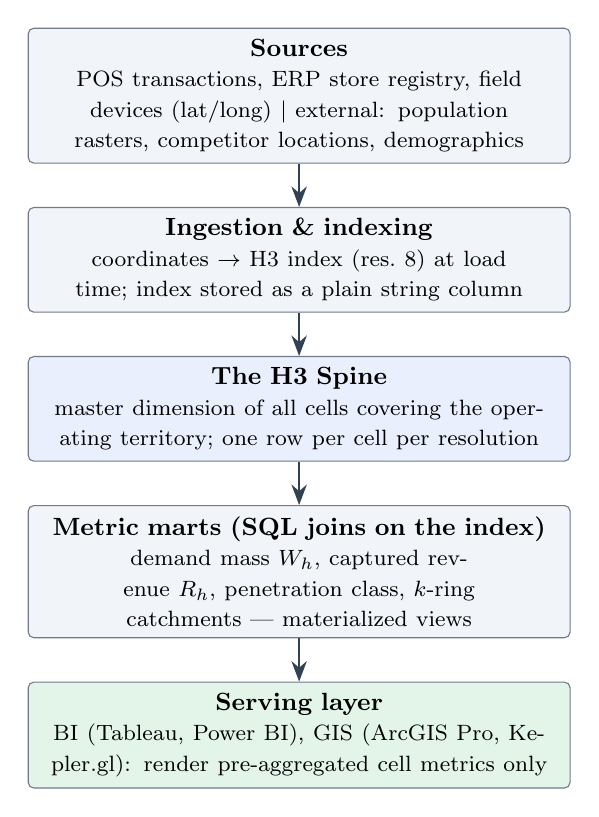
\begin{tikzpicture}[node distance=0.55cm]
    \node[spineblock, text width=6.6cm] (src)
      {\textbf{Sources}\\
       \footnotesize POS transactions, ERP store registry, field devices
       (lat/long) $\mid$ external: population rasters, competitor
       locations, demographics};
    \node[spineblock, text width=6.6cm, below=of src] (ingest)
      {\textbf{Ingestion \& indexing}\\
       \footnotesize coordinates $\rightarrow$ H3 index (res.\ 8) at load
       time; index stored as a plain string column};
    \node[spineblock, text width=6.6cm, fill=spineBlue!10, below=of ingest]
      (spine)
      {\textbf{The H3 Spine}\\
       \footnotesize master dimension of all cells covering the operating
       territory; one row per cell per resolution};
    \node[spineblock, text width=6.6cm, below=of spine] (marts)
      {\textbf{Metric marts (SQL joins on the index)}\\
       \footnotesize demand mass $W_h$, captured revenue $R_h$,
       penetration class, $k$-ring catchments --- materialized views};
    \node[spineblock, text width=6.6cm, fill=spineGreen!12, below=of marts]
      (viz)
      {\textbf{Serving layer}\\
       \footnotesize BI (Tableau, Power BI), GIS (ArcGIS Pro, Kepler.gl):
       render pre-aggregated cell metrics only};
    \draw[spinearrow] (src) -- (ingest);
    \draw[spinearrow] (ingest) -- (spine);
    \draw[spinearrow] (spine) -- (marts);
    \draw[spinearrow] (marts) -- (viz);
  \end{tikzpicture}
  \caption{The H3 Spine pipeline. Indexing happens once at ingestion;
    every downstream operation is a join on the H3 string, and
    visualization tools render pre-aggregated metrics rather than raw
    geometry.}
  \label{fig:pipeline}
\end{figure}

\textbf{Index at ingestion, never at query time.} Coordinates from POS
systems, ERP store masters, and field devices are converted to a
resolution-8 H3 string the moment they land. Geocoding debt is paid once;
every analyst thereafter inherits a clean join key. External layers ---
open population data already distributed on H3 cells~\cite{kontur},
competitor registries, demographics --- are transformed to the same
resolution on arrival.

\textbf{One spine, many resolutions.} The master dimension holds every
cell covering the operating territory. Because aperture-7 parentage is a
function of the index, coarser rollups are derived columns, not separate
pipelines. The spine also carries slowly changing cell attributes
(urban/rural class, region ownership, serviceability flags) so that
business rules join at the same key as facts.

\textbf{Metrics as materialized views.} The analytical layer of
Section~\ref{sec:method} compiles to ordinary SQL over the spine ---
group-bys, window percentiles, and bounded \texttt{k-ring} expansions ---
maintained as scheduled materialized views. BI and GIS tools connect to
these views and render \emph{pre-aggregated} cell metrics, which keeps
dashboards fast, load predictable, and governance centralized: there is
exactly one definition of ``whitespace'' in the company, and it lives in
the warehouse, not in a workbook.

% ============================================================================
\section{Analytical Method}
\label{sec:method}

We now define the metrics layer. All quantities are per-cell; $h$ ranges
over spine cells and $s$ over stores. Table~\ref{tab:notation} collects
the notation.

\begin{table}[t]
  \centering
  \small
  \caption{Notation.}
  \label{tab:notation}
  \begin{tabular}{@{}ll@{}}
    \toprule
    \textbf{Symbol} & \textbf{Meaning} \\
    \midrule
    $H$, $S$ & set of spine cells / stores \\
    $P_h$ & population of cell $h$ \\
    $a_s$ & attractiveness (gross pull) of store $s$ \\
    $d(h,s)$ & hex-grid distance, cell $h$ to store cell \\
    $\tau$ & catchment decay length (cells) \\
    $\kappa$ & spend conversion rate (IDR/person) \\
    $R_h$ & monthly revenue captured from cell $h$ \\
    $r_h$ & revenue per capita, $R_h / P_h$ \\
    $P^{*}, r^{*}$ & population / rev-per-capita thresholds \\
    $\mathcal{K}_k(s)$ & $k$-ring catchment of store $s$ \\
    $G(x)$ & population reached at area share $x$ \\
    $W_h$ & composite demand mass of cell $h$ \\
    \bottomrule
  \end{tabular}
\end{table}

\subsection{Demand Surface}

The base layer is a population (or, more generally, demand) surface on the
spine. Where richer signals exist, a composite mass generalizes raw
population:
\begin{equation}
  \label{eq:mass}
  W_h \;=\; \lambda_P P_h + \lambda_O O_h + \lambda_S S_h,
\end{equation}
with $O_h$ historical order volume, $S_h$ serviceable-outlet density, and
$\lambda$'s business-set calibration weights --- the same composite that
feeds the routing layer in~\cite{terra2026}. The case study uses the pure
population surface ($\lambda_O = \lambda_S = 0$), which is the honest
starting point for an organization bootstrapping the spine from open
data~\cite{kontur}.

\subsection{Revenue Capture with Distance Decay}

Each store projects a Huff-style~\cite{huff1964} Gaussian decay kernel
onto the surrounding cells; the revenue captured from cell $h$ is
\begin{equation}
  \label{eq:capture}
  R_h \;=\; \kappa \, P_h \sum_{s \in S} a_s\,
    \exp\!\left( -\frac{d(h,s)^2}{2\tau^2} \right),
\end{equation}
truncated to zero below a floor $\varepsilon$ (a cell whose entire
predicted capture is negligible is treated as unserved). The decay length
$\tau$ is the single most consequential calibration: it encodes how far
consumers travel to a store, and should be fit per store format from
loyalty or delivery-address data. Note that $d(h,s)$ is the \emph{hex-grid}
distance --- a constant-time index computation on the spine, not a road
query; where road realism matters the kernel can be re-evaluated on
travel-time isochrones without changing anything downstream.

\subsection{Penetration Classification}

Cells are classified by crossing the demand surface with captured revenue.
With $P^{*}$ a population percentile threshold (the case study uses the
60th) and $r^{*}$ a per-capita revenue threshold (40th percentile of
served cells), rules evaluated top to bottom:
\begin{equation}
  \label{eq:class}
  \mathrm{class}(h) =
  \begin{cases}
    \text{low priority}, & P_h < P^{*},\\[0.2em]
    \text{whitespace}, & R_h = 0,\\[0.2em]
    \text{under-penetrated}, & r_h < r^{*},\\[0.2em]
    \text{penetrated}, & \text{otherwise.}
  \end{cases}
\end{equation}
The taxonomy is deliberately coarse --- four classes an executive can act
on. \emph{Whitespace} (people, no revenue) is the expansion shortlist;
\emph{under-penetrated} (people, weak revenue) is the marketing and
assortment shortlist; the thresholds are percentile-based so the
classification survives recalibration of $\kappa$ and $a_s$ unchanged.
The monetary size of the whitespace follows directly: at the served-cell
average revenue per capita $\bar{r}$, the opportunity is
$\bar{r} \sum_{h \in \mathrm{white}} P_h$.

\subsection{$k$-Ring Catchments and Cannibalization}

The $k$-ring $\mathcal{K}_k(s) = \{\,h : d(h,s) \le k\,\}$ is the spine's
native catchment primitive. For two stores, the shared cells
$\mathcal{K}_k(s) \cap \mathcal{K}_k(s')$ measure catchment overlap; the
population-weighted overlap share
\begin{equation}
  \label{eq:cannibal}
  \chi(s,s') \;=\;
  \frac{\sum_{h \in \mathcal{K}_k(s) \cap \mathcal{K}_k(s')} P_h}
       {\sum_{h \in \mathcal{K}_k(s)} P_h}
\end{equation}
is a direct cannibalization index, computable before a candidate site is
committed (Figure~\ref{fig:kring}). The same primitive defines
fulfillment zones for distribution centers and dispatch clusters for
field-service teams.

\subsection{Targeting Gain Curves}

Finally, the spine makes targeting efficiency measurable. Rank cells by
descending $P_h$ and let $G(x)$ be the share of total population contained
in the top $x$ share of land area; the administrative counterpart ranks
whole districts by mean density and accumulates entire polygons. The gap
between the two curves (Figure~\ref{fig:gain}) is the price of being
forced to buy geography in district-sized blocks --- it bounds the
achievable precision of geofenced media, sampling campaigns, and coverage
commitments under each geography.

\begin{figure}[t]
  \centering
  \resizebox{\columnwidth}{!}{% Auto-generated by generate_figures.py -- do not edit by hand
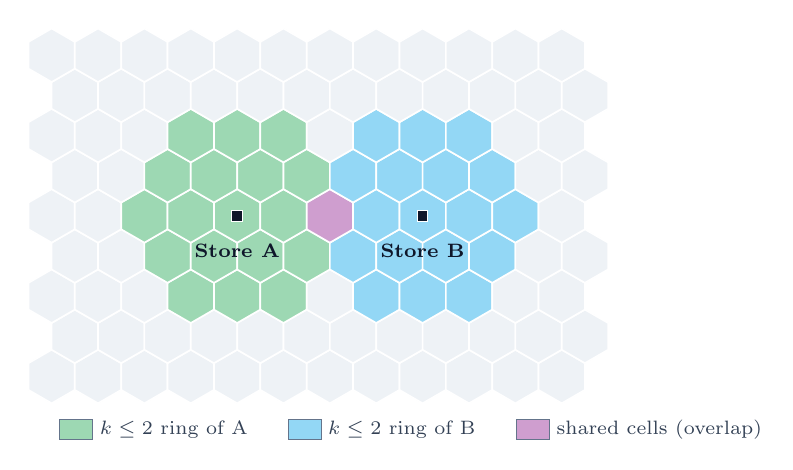
\begin{tikzpicture}
\fill[neu, draw=white, line width=0.6pt] (0.294,0.170) -- (0.000,0.340) -- (-0.294,0.170) -- (-0.294,-0.170) -- (-0.000,-0.340) -- (0.294,-0.170) -- cycle;
\fill[neu, draw=white, line width=0.6pt] (0.883,0.170) -- (0.589,0.340) -- (0.294,0.170) -- (0.294,-0.170) -- (0.589,-0.340) -- (0.883,-0.170) -- cycle;
\fill[neu, draw=white, line width=0.6pt] (1.472,0.170) -- (1.178,0.340) -- (0.883,0.170) -- (0.883,-0.170) -- (1.178,-0.340) -- (1.472,-0.170) -- cycle;
\fill[neu, draw=white, line width=0.6pt] (2.061,0.170) -- (1.767,0.340) -- (1.472,0.170) -- (1.472,-0.170) -- (1.767,-0.340) -- (2.061,-0.170) -- cycle;
\fill[neu, draw=white, line width=0.6pt] (2.650,0.170) -- (2.356,0.340) -- (2.061,0.170) -- (2.061,-0.170) -- (2.356,-0.340) -- (2.650,-0.170) -- cycle;
\fill[neu, draw=white, line width=0.6pt] (3.239,0.170) -- (2.944,0.340) -- (2.650,0.170) -- (2.650,-0.170) -- (2.944,-0.340) -- (3.239,-0.170) -- cycle;
\fill[neu, draw=white, line width=0.6pt] (3.828,0.170) -- (3.533,0.340) -- (3.239,0.170) -- (3.239,-0.170) -- (3.533,-0.340) -- (3.828,-0.170) -- cycle;
\fill[neu, draw=white, line width=0.6pt] (4.417,0.170) -- (4.122,0.340) -- (3.828,0.170) -- (3.828,-0.170) -- (4.122,-0.340) -- (4.417,-0.170) -- cycle;
\fill[neu, draw=white, line width=0.6pt] (5.006,0.170) -- (4.711,0.340) -- (4.417,0.170) -- (4.417,-0.170) -- (4.711,-0.340) -- (5.006,-0.170) -- cycle;
\fill[neu, draw=white, line width=0.6pt] (5.595,0.170) -- (5.300,0.340) -- (5.006,0.170) -- (5.006,-0.170) -- (5.300,-0.340) -- (5.595,-0.170) -- cycle;
\fill[neu, draw=white, line width=0.6pt] (6.183,0.170) -- (5.889,0.340) -- (5.595,0.170) -- (5.595,-0.170) -- (5.889,-0.340) -- (6.183,-0.170) -- cycle;
\fill[neu, draw=white, line width=0.6pt] (6.772,0.170) -- (6.478,0.340) -- (6.183,0.170) -- (6.183,-0.170) -- (6.478,-0.340) -- (6.772,-0.170) -- cycle;
\fill[neu, draw=white, line width=0.6pt] (0.589,0.680) -- (0.294,0.850) -- (0.000,0.680) -- (0.000,0.340) -- (0.294,0.170) -- (0.589,0.340) -- cycle;
\fill[neu, draw=white, line width=0.6pt] (1.178,0.680) -- (0.883,0.850) -- (0.589,0.680) -- (0.589,0.340) -- (0.883,0.170) -- (1.178,0.340) -- cycle;
\fill[neu, draw=white, line width=0.6pt] (1.767,0.680) -- (1.472,0.850) -- (1.178,0.680) -- (1.178,0.340) -- (1.472,0.170) -- (1.767,0.340) -- cycle;
\fill[neu, draw=white, line width=0.6pt] (2.356,0.680) -- (2.061,0.850) -- (1.767,0.680) -- (1.767,0.340) -- (2.061,0.170) -- (2.356,0.340) -- cycle;
\fill[neu, draw=white, line width=0.6pt] (2.944,0.680) -- (2.650,0.850) -- (2.356,0.680) -- (2.356,0.340) -- (2.650,0.170) -- (2.944,0.340) -- cycle;
\fill[neu, draw=white, line width=0.6pt] (3.533,0.680) -- (3.239,0.850) -- (2.944,0.680) -- (2.944,0.340) -- (3.239,0.170) -- (3.533,0.340) -- cycle;
\fill[neu, draw=white, line width=0.6pt] (4.122,0.680) -- (3.828,0.850) -- (3.533,0.680) -- (3.533,0.340) -- (3.828,0.170) -- (4.122,0.340) -- cycle;
\fill[neu, draw=white, line width=0.6pt] (4.711,0.680) -- (4.417,0.850) -- (4.122,0.680) -- (4.122,0.340) -- (4.417,0.170) -- (4.711,0.340) -- cycle;
\fill[neu, draw=white, line width=0.6pt] (5.300,0.680) -- (5.006,0.850) -- (4.711,0.680) -- (4.711,0.340) -- (5.006,0.170) -- (5.300,0.340) -- cycle;
\fill[neu, draw=white, line width=0.6pt] (5.889,0.680) -- (5.595,0.850) -- (5.300,0.680) -- (5.300,0.340) -- (5.595,0.170) -- (5.889,0.340) -- cycle;
\fill[neu, draw=white, line width=0.6pt] (6.478,0.680) -- (6.183,0.850) -- (5.889,0.680) -- (5.889,0.340) -- (6.183,0.170) -- (6.478,0.340) -- cycle;
\fill[neu, draw=white, line width=0.6pt] (7.067,0.680) -- (6.772,0.850) -- (6.478,0.680) -- (6.478,0.340) -- (6.772,0.170) -- (7.067,0.340) -- cycle;
\fill[neu, draw=white, line width=0.6pt] (0.294,1.190) -- (0.000,1.360) -- (-0.294,1.190) -- (-0.294,0.850) -- (-0.000,0.680) -- (0.294,0.850) -- cycle;
\fill[neu, draw=white, line width=0.6pt] (0.883,1.190) -- (0.589,1.360) -- (0.294,1.190) -- (0.294,0.850) -- (0.589,0.680) -- (0.883,0.850) -- cycle;
\fill[neu, draw=white, line width=0.6pt] (1.472,1.190) -- (1.178,1.360) -- (0.883,1.190) -- (0.883,0.850) -- (1.178,0.680) -- (1.472,0.850) -- cycle;
\fill[clsPen!42!white, draw=white, line width=0.6pt] (2.061,1.190) -- (1.767,1.360) -- (1.472,1.190) -- (1.472,0.850) -- (1.767,0.680) -- (2.061,0.850) -- cycle;
\fill[clsPen!42!white, draw=white, line width=0.6pt] (2.650,1.190) -- (2.356,1.360) -- (2.061,1.190) -- (2.061,0.850) -- (2.356,0.680) -- (2.650,0.850) -- cycle;
\fill[clsPen!42!white, draw=white, line width=0.6pt] (3.239,1.190) -- (2.944,1.360) -- (2.650,1.190) -- (2.650,0.850) -- (2.944,0.680) -- (3.239,0.850) -- cycle;
\fill[neu, draw=white, line width=0.6pt] (3.828,1.190) -- (3.533,1.360) -- (3.239,1.190) -- (3.239,0.850) -- (3.533,0.680) -- (3.828,0.850) -- cycle;
\fill[aqua!45!white, draw=white, line width=0.6pt] (4.417,1.190) -- (4.122,1.360) -- (3.828,1.190) -- (3.828,0.850) -- (4.122,0.680) -- (4.417,0.850) -- cycle;
\fill[aqua!45!white, draw=white, line width=0.6pt] (5.006,1.190) -- (4.711,1.360) -- (4.417,1.190) -- (4.417,0.850) -- (4.711,0.680) -- (5.006,0.850) -- cycle;
\fill[aqua!45!white, draw=white, line width=0.6pt] (5.595,1.190) -- (5.300,1.360) -- (5.006,1.190) -- (5.006,0.850) -- (5.300,0.680) -- (5.595,0.850) -- cycle;
\fill[neu, draw=white, line width=0.6pt] (6.183,1.190) -- (5.889,1.360) -- (5.595,1.190) -- (5.595,0.850) -- (5.889,0.680) -- (6.183,0.850) -- cycle;
\fill[neu, draw=white, line width=0.6pt] (6.772,1.190) -- (6.478,1.360) -- (6.183,1.190) -- (6.183,0.850) -- (6.478,0.680) -- (6.772,0.850) -- cycle;
\fill[neu, draw=white, line width=0.6pt] (0.589,1.700) -- (0.294,1.870) -- (0.000,1.700) -- (0.000,1.360) -- (0.294,1.190) -- (0.589,1.360) -- cycle;
\fill[neu, draw=white, line width=0.6pt] (1.178,1.700) -- (0.883,1.870) -- (0.589,1.700) -- (0.589,1.360) -- (0.883,1.190) -- (1.178,1.360) -- cycle;
\fill[clsPen!42!white, draw=white, line width=0.6pt] (1.767,1.700) -- (1.472,1.870) -- (1.178,1.700) -- (1.178,1.360) -- (1.472,1.190) -- (1.767,1.360) -- cycle;
\fill[clsPen!42!white, draw=white, line width=0.6pt] (2.356,1.700) -- (2.061,1.870) -- (1.767,1.700) -- (1.767,1.360) -- (2.061,1.190) -- (2.356,1.360) -- cycle;
\fill[clsPen!42!white, draw=white, line width=0.6pt] (2.944,1.700) -- (2.650,1.870) -- (2.356,1.700) -- (2.356,1.360) -- (2.650,1.190) -- (2.944,1.360) -- cycle;
\fill[clsPen!42!white, draw=white, line width=0.6pt] (3.533,1.700) -- (3.239,1.870) -- (2.944,1.700) -- (2.944,1.360) -- (3.239,1.190) -- (3.533,1.360) -- cycle;
\fill[aqua!45!white, draw=white, line width=0.6pt] (4.122,1.700) -- (3.828,1.870) -- (3.533,1.700) -- (3.533,1.360) -- (3.828,1.190) -- (4.122,1.360) -- cycle;
\fill[aqua!45!white, draw=white, line width=0.6pt] (4.711,1.700) -- (4.417,1.870) -- (4.122,1.700) -- (4.122,1.360) -- (4.417,1.190) -- (4.711,1.360) -- cycle;
\fill[aqua!45!white, draw=white, line width=0.6pt] (5.300,1.700) -- (5.006,1.870) -- (4.711,1.700) -- (4.711,1.360) -- (5.006,1.190) -- (5.300,1.360) -- cycle;
\fill[aqua!45!white, draw=white, line width=0.6pt] (5.889,1.700) -- (5.595,1.870) -- (5.300,1.700) -- (5.300,1.360) -- (5.595,1.190) -- (5.889,1.360) -- cycle;
\fill[neu, draw=white, line width=0.6pt] (6.478,1.700) -- (6.183,1.870) -- (5.889,1.700) -- (5.889,1.360) -- (6.183,1.190) -- (6.478,1.360) -- cycle;
\fill[neu, draw=white, line width=0.6pt] (7.067,1.700) -- (6.772,1.870) -- (6.478,1.700) -- (6.478,1.360) -- (6.772,1.190) -- (7.067,1.360) -- cycle;
\fill[neu, draw=white, line width=0.6pt] (0.294,2.210) -- (0.000,2.380) -- (-0.294,2.210) -- (-0.294,1.870) -- (-0.000,1.700) -- (0.294,1.870) -- cycle;
\fill[neu, draw=white, line width=0.6pt] (0.883,2.210) -- (0.589,2.380) -- (0.294,2.210) -- (0.294,1.870) -- (0.589,1.700) -- (0.883,1.870) -- cycle;
\fill[clsPen!42!white, draw=white, line width=0.6pt] (1.472,2.210) -- (1.178,2.380) -- (0.883,2.210) -- (0.883,1.870) -- (1.178,1.700) -- (1.472,1.870) -- cycle;
\fill[clsPen!42!white, draw=white, line width=0.6pt] (2.061,2.210) -- (1.767,2.380) -- (1.472,2.210) -- (1.472,1.870) -- (1.767,1.700) -- (2.061,1.870) -- cycle;
\fill[clsPen!42!white, draw=white, line width=0.6pt] (2.650,2.210) -- (2.356,2.380) -- (2.061,2.210) -- (2.061,1.870) -- (2.356,1.700) -- (2.650,1.870) -- cycle;
\fill[clsPen!42!white, draw=white, line width=0.6pt] (3.239,2.210) -- (2.944,2.380) -- (2.650,2.210) -- (2.650,1.870) -- (2.944,1.700) -- (3.239,1.870) -- cycle;
\fill[violet!38!white, draw=white, line width=0.6pt] (3.828,2.210) -- (3.533,2.380) -- (3.239,2.210) -- (3.239,1.870) -- (3.533,1.700) -- (3.828,1.870) -- cycle;
\fill[aqua!45!white, draw=white, line width=0.6pt] (4.417,2.210) -- (4.122,2.380) -- (3.828,2.210) -- (3.828,1.870) -- (4.122,1.700) -- (4.417,1.870) -- cycle;
\fill[aqua!45!white, draw=white, line width=0.6pt] (5.006,2.210) -- (4.711,2.380) -- (4.417,2.210) -- (4.417,1.870) -- (4.711,1.700) -- (5.006,1.870) -- cycle;
\fill[aqua!45!white, draw=white, line width=0.6pt] (5.595,2.210) -- (5.300,2.380) -- (5.006,2.210) -- (5.006,1.870) -- (5.300,1.700) -- (5.595,1.870) -- cycle;
\fill[aqua!45!white, draw=white, line width=0.6pt] (6.183,2.210) -- (5.889,2.380) -- (5.595,2.210) -- (5.595,1.870) -- (5.889,1.700) -- (6.183,1.870) -- cycle;
\fill[neu, draw=white, line width=0.6pt] (6.772,2.210) -- (6.478,2.380) -- (6.183,2.210) -- (6.183,1.870) -- (6.478,1.700) -- (6.772,1.870) -- cycle;
\fill[neu, draw=white, line width=0.6pt] (0.589,2.720) -- (0.294,2.890) -- (0.000,2.720) -- (0.000,2.380) -- (0.294,2.210) -- (0.589,2.380) -- cycle;
\fill[neu, draw=white, line width=0.6pt] (1.178,2.720) -- (0.883,2.890) -- (0.589,2.720) -- (0.589,2.380) -- (0.883,2.210) -- (1.178,2.380) -- cycle;
\fill[clsPen!42!white, draw=white, line width=0.6pt] (1.767,2.720) -- (1.472,2.890) -- (1.178,2.720) -- (1.178,2.380) -- (1.472,2.210) -- (1.767,2.380) -- cycle;
\fill[clsPen!42!white, draw=white, line width=0.6pt] (2.356,2.720) -- (2.061,2.890) -- (1.767,2.720) -- (1.767,2.380) -- (2.061,2.210) -- (2.356,2.380) -- cycle;
\fill[clsPen!42!white, draw=white, line width=0.6pt] (2.944,2.720) -- (2.650,2.890) -- (2.356,2.720) -- (2.356,2.380) -- (2.650,2.210) -- (2.944,2.380) -- cycle;
\fill[clsPen!42!white, draw=white, line width=0.6pt] (3.533,2.720) -- (3.239,2.890) -- (2.944,2.720) -- (2.944,2.380) -- (3.239,2.210) -- (3.533,2.380) -- cycle;
\fill[aqua!45!white, draw=white, line width=0.6pt] (4.122,2.720) -- (3.828,2.890) -- (3.533,2.720) -- (3.533,2.380) -- (3.828,2.210) -- (4.122,2.380) -- cycle;
\fill[aqua!45!white, draw=white, line width=0.6pt] (4.711,2.720) -- (4.417,2.890) -- (4.122,2.720) -- (4.122,2.380) -- (4.417,2.210) -- (4.711,2.380) -- cycle;
\fill[aqua!45!white, draw=white, line width=0.6pt] (5.300,2.720) -- (5.006,2.890) -- (4.711,2.720) -- (4.711,2.380) -- (5.006,2.210) -- (5.300,2.380) -- cycle;
\fill[aqua!45!white, draw=white, line width=0.6pt] (5.889,2.720) -- (5.595,2.890) -- (5.300,2.720) -- (5.300,2.380) -- (5.595,2.210) -- (5.889,2.380) -- cycle;
\fill[neu, draw=white, line width=0.6pt] (6.478,2.720) -- (6.183,2.890) -- (5.889,2.720) -- (5.889,2.380) -- (6.183,2.210) -- (6.478,2.380) -- cycle;
\fill[neu, draw=white, line width=0.6pt] (7.067,2.720) -- (6.772,2.890) -- (6.478,2.720) -- (6.478,2.380) -- (6.772,2.210) -- (7.067,2.380) -- cycle;
\fill[neu, draw=white, line width=0.6pt] (0.294,3.230) -- (0.000,3.400) -- (-0.294,3.230) -- (-0.294,2.890) -- (-0.000,2.720) -- (0.294,2.890) -- cycle;
\fill[neu, draw=white, line width=0.6pt] (0.883,3.230) -- (0.589,3.400) -- (0.294,3.230) -- (0.294,2.890) -- (0.589,2.720) -- (0.883,2.890) -- cycle;
\fill[neu, draw=white, line width=0.6pt] (1.472,3.230) -- (1.178,3.400) -- (0.883,3.230) -- (0.883,2.890) -- (1.178,2.720) -- (1.472,2.890) -- cycle;
\fill[clsPen!42!white, draw=white, line width=0.6pt] (2.061,3.230) -- (1.767,3.400) -- (1.472,3.230) -- (1.472,2.890) -- (1.767,2.720) -- (2.061,2.890) -- cycle;
\fill[clsPen!42!white, draw=white, line width=0.6pt] (2.650,3.230) -- (2.356,3.400) -- (2.061,3.230) -- (2.061,2.890) -- (2.356,2.720) -- (2.650,2.890) -- cycle;
\fill[clsPen!42!white, draw=white, line width=0.6pt] (3.239,3.230) -- (2.944,3.400) -- (2.650,3.230) -- (2.650,2.890) -- (2.944,2.720) -- (3.239,2.890) -- cycle;
\fill[neu, draw=white, line width=0.6pt] (3.828,3.230) -- (3.533,3.400) -- (3.239,3.230) -- (3.239,2.890) -- (3.533,2.720) -- (3.828,2.890) -- cycle;
\fill[aqua!45!white, draw=white, line width=0.6pt] (4.417,3.230) -- (4.122,3.400) -- (3.828,3.230) -- (3.828,2.890) -- (4.122,2.720) -- (4.417,2.890) -- cycle;
\fill[aqua!45!white, draw=white, line width=0.6pt] (5.006,3.230) -- (4.711,3.400) -- (4.417,3.230) -- (4.417,2.890) -- (4.711,2.720) -- (5.006,2.890) -- cycle;
\fill[aqua!45!white, draw=white, line width=0.6pt] (5.595,3.230) -- (5.300,3.400) -- (5.006,3.230) -- (5.006,2.890) -- (5.300,2.720) -- (5.595,2.890) -- cycle;
\fill[neu, draw=white, line width=0.6pt] (6.183,3.230) -- (5.889,3.400) -- (5.595,3.230) -- (5.595,2.890) -- (5.889,2.720) -- (6.183,2.890) -- cycle;
\fill[neu, draw=white, line width=0.6pt] (6.772,3.230) -- (6.478,3.400) -- (6.183,3.230) -- (6.183,2.890) -- (6.478,2.720) -- (6.772,2.890) -- cycle;
\fill[neu, draw=white, line width=0.6pt] (0.589,3.740) -- (0.294,3.910) -- (0.000,3.740) -- (0.000,3.400) -- (0.294,3.230) -- (0.589,3.400) -- cycle;
\fill[neu, draw=white, line width=0.6pt] (1.178,3.740) -- (0.883,3.910) -- (0.589,3.740) -- (0.589,3.400) -- (0.883,3.230) -- (1.178,3.400) -- cycle;
\fill[neu, draw=white, line width=0.6pt] (1.767,3.740) -- (1.472,3.910) -- (1.178,3.740) -- (1.178,3.400) -- (1.472,3.230) -- (1.767,3.400) -- cycle;
\fill[neu, draw=white, line width=0.6pt] (2.356,3.740) -- (2.061,3.910) -- (1.767,3.740) -- (1.767,3.400) -- (2.061,3.230) -- (2.356,3.400) -- cycle;
\fill[neu, draw=white, line width=0.6pt] (2.944,3.740) -- (2.650,3.910) -- (2.356,3.740) -- (2.356,3.400) -- (2.650,3.230) -- (2.944,3.400) -- cycle;
\fill[neu, draw=white, line width=0.6pt] (3.533,3.740) -- (3.239,3.910) -- (2.944,3.740) -- (2.944,3.400) -- (3.239,3.230) -- (3.533,3.400) -- cycle;
\fill[neu, draw=white, line width=0.6pt] (4.122,3.740) -- (3.828,3.910) -- (3.533,3.740) -- (3.533,3.400) -- (3.828,3.230) -- (4.122,3.400) -- cycle;
\fill[neu, draw=white, line width=0.6pt] (4.711,3.740) -- (4.417,3.910) -- (4.122,3.740) -- (4.122,3.400) -- (4.417,3.230) -- (4.711,3.400) -- cycle;
\fill[neu, draw=white, line width=0.6pt] (5.300,3.740) -- (5.006,3.910) -- (4.711,3.740) -- (4.711,3.400) -- (5.006,3.230) -- (5.300,3.400) -- cycle;
\fill[neu, draw=white, line width=0.6pt] (5.889,3.740) -- (5.595,3.910) -- (5.300,3.740) -- (5.300,3.400) -- (5.595,3.230) -- (5.889,3.400) -- cycle;
\fill[neu, draw=white, line width=0.6pt] (6.478,3.740) -- (6.183,3.910) -- (5.889,3.740) -- (5.889,3.400) -- (6.183,3.230) -- (6.478,3.400) -- cycle;
\fill[neu, draw=white, line width=0.6pt] (7.067,3.740) -- (6.772,3.910) -- (6.478,3.740) -- (6.478,3.400) -- (6.772,3.230) -- (7.067,3.400) -- cycle;
\fill[neu, draw=white, line width=0.6pt] (0.294,4.250) -- (0.000,4.420) -- (-0.294,4.250) -- (-0.294,3.910) -- (-0.000,3.740) -- (0.294,3.910) -- cycle;
\fill[neu, draw=white, line width=0.6pt] (0.883,4.250) -- (0.589,4.420) -- (0.294,4.250) -- (0.294,3.910) -- (0.589,3.740) -- (0.883,3.910) -- cycle;
\fill[neu, draw=white, line width=0.6pt] (1.472,4.250) -- (1.178,4.420) -- (0.883,4.250) -- (0.883,3.910) -- (1.178,3.740) -- (1.472,3.910) -- cycle;
\fill[neu, draw=white, line width=0.6pt] (2.061,4.250) -- (1.767,4.420) -- (1.472,4.250) -- (1.472,3.910) -- (1.767,3.740) -- (2.061,3.910) -- cycle;
\fill[neu, draw=white, line width=0.6pt] (2.650,4.250) -- (2.356,4.420) -- (2.061,4.250) -- (2.061,3.910) -- (2.356,3.740) -- (2.650,3.910) -- cycle;
\fill[neu, draw=white, line width=0.6pt] (3.239,4.250) -- (2.944,4.420) -- (2.650,4.250) -- (2.650,3.910) -- (2.944,3.740) -- (3.239,3.910) -- cycle;
\fill[neu, draw=white, line width=0.6pt] (3.828,4.250) -- (3.533,4.420) -- (3.239,4.250) -- (3.239,3.910) -- (3.533,3.740) -- (3.828,3.910) -- cycle;
\fill[neu, draw=white, line width=0.6pt] (4.417,4.250) -- (4.122,4.420) -- (3.828,4.250) -- (3.828,3.910) -- (4.122,3.740) -- (4.417,3.910) -- cycle;
\fill[neu, draw=white, line width=0.6pt] (5.006,4.250) -- (4.711,4.420) -- (4.417,4.250) -- (4.417,3.910) -- (4.711,3.740) -- (5.006,3.910) -- cycle;
\fill[neu, draw=white, line width=0.6pt] (5.595,4.250) -- (5.300,4.420) -- (5.006,4.250) -- (5.006,3.910) -- (5.300,3.740) -- (5.595,3.910) -- cycle;
\fill[neu, draw=white, line width=0.6pt] (6.183,4.250) -- (5.889,4.420) -- (5.595,4.250) -- (5.595,3.910) -- (5.889,3.740) -- (6.183,3.910) -- cycle;
\fill[neu, draw=white, line width=0.6pt] (6.772,4.250) -- (6.478,4.420) -- (6.183,4.250) -- (6.183,3.910) -- (6.478,3.740) -- (6.772,3.910) -- cycle;
\node[store] at (2.356,2.040) {};
\node[font=\scriptsize\bfseries, text=inkP, anchor=north] at (2.356,1.800) {Store A};
\node[store] at (4.711,2.040) {};
\node[font=\scriptsize\bfseries, text=inkP, anchor=north] at (4.711,1.800) {Store B};
\fill[clsPen!42!white, draw=inkM, line width=0.2pt] (0.100,-0.800) rectangle (0.520,-0.540);
\node[anchor=west, font=\scriptsize, text=inkS, inner sep=1pt] at (0.570,-0.670) {$k\le2$ ring of A};
\fill[aqua!45!white, draw=inkM, line width=0.2pt] (3.000,-0.800) rectangle (3.420,-0.540);
\node[anchor=west, font=\scriptsize, text=inkS, inner sep=1pt] at (3.470,-0.670) {$k\le2$ ring of B};
\fill[violet!38!white, draw=inkM, line width=0.2pt] (5.900,-0.800) rectangle (6.320,-0.540);
\node[anchor=west, font=\scriptsize, text=inkS, inner sep=1pt] at (6.370,-0.670) {shared cells (overlap)};
\end{tikzpicture}
}
  \caption{$k$-ring catchment overlap between two stores four cells apart:
    cells within $k \le 2$ of each store, with the shared cell marking the
    cannibalization zone.}
  \label{fig:kring}
\end{figure}

% ============================================================================
\section{Case Study: The Western Jakarta--Tangerang Corridor}
\label{sec:casestudy}

We exercise the full spine workflow on a deterministic synthetic corridor
styled on the western Jakarta--Tangerang conurbation: 232 land cells at
resolution~8 (${\sim}171$\,km$^2$) between a masked Java Sea coastline and
an inland fringe, holding 1.61 million synthetic residents. The surface
composites five density centers --- a CBD core, western
(``Tangerang-side''), eastern, and southern sub-centers, and an infill
corridor --- over a noisy urban baseline. Twelve stores (S01--S12) cluster
in the CBD, the west, and the south; \emph{the eastern sub-center has
none}, a deliberate gap the analysis should rediscover. All data are
generated by a seeded script (\texttt{generate\_figures.py}), so every
number and figure in this section is exactly reproducible; the workflow,
not the synthetic magnitudes, is the claim being demonstrated.

\subsection{Layer 1: Population}

Figure~\ref{fig:population} shows the demand surface with the store
network overlaid. Even at a glance the resolution-8 grid conveys what
district aggregation cannot (compare Figure~\ref{fig:maup}a): the CBD
gradient, the three secondary peaks, and the store network's western bias
are all legible because every cell is the same size.

\subsection{Layer 2: Revenue, Joined on the Spine}

Applying the capture model of Eq.~\eqref{eq:capture} with decay length
$\tau = 1.55$ cells (${\sim}1.5$\,km) yields IDR~507.8\,bn of monthly
revenue attributed across cells --- Figure~\ref{fig:overlay} renders it as
bubbles over the population fill. The join that produces this figure is
one line of SQL on the spine: revenue facts and population both keyed by
the same H3 string. The overlay already telegraphs the finding: the
eastern population peak carries essentially no revenue mass, and its
cells are outlined as whitespace.

\subsection{Layer 3: Classification}

Applying Eq.~\eqref{eq:class} with the 60th-percentile population
threshold ($P^{*} = 7{,}076$ per cell) and the 40th-percentile per-capita
revenue threshold ($r^{*} = $ IDR~136{,}472/person/month) partitions the
corridor into 77 penetrated, 13 under-penetrated, 3 whitespace, and 139
low-priority cells (Figure~\ref{fig:classification}). The scatter view
(Figure~\ref{fig:scatter}) shows the same partition in metric space:
whitespace cells sit far right on the population axis at exactly zero
captured revenue --- populous, unserved, and invisible to any analysis
keyed on served territory.

\subsection{Sizing the Opportunity}

The three whitespace cells hold 23{,}210 residents --- only 1.4\% of
corridor population, but concentrated in the eastern sub-center at
walkable density. At the served-cell average of IDR~361{,}662 per person
per month, closing them is worth ${\sim}$IDR~8.4\,bn of monthly revenue,
before counting the 13 under-penetrated cells (136{,}164 residents
currently monetizing below $r^{*}$). This is the strategic deliverable of
the spine: not a map, but a ranked, priced shortlist of cells --- each
${\sim}0.74$\,km$^2$, small enough to visit, audit, and act on.

\begin{figure*}[t]
  \centering
  \resizebox{0.86\textwidth}{!}{\input{figures/fig-population.tex}}
  \caption{Synthetic population surface of the study corridor on H3
    resolution-8 cells (${\sim}0.74$\,km$^2$ each), with the existing store
    network overlaid.}
  \label{fig:population}
\end{figure*}

\begin{figure*}[t]
  \centering
  \resizebox{0.86\textwidth}{!}{% Auto-generated by generate_figures.py -- do not edit by hand
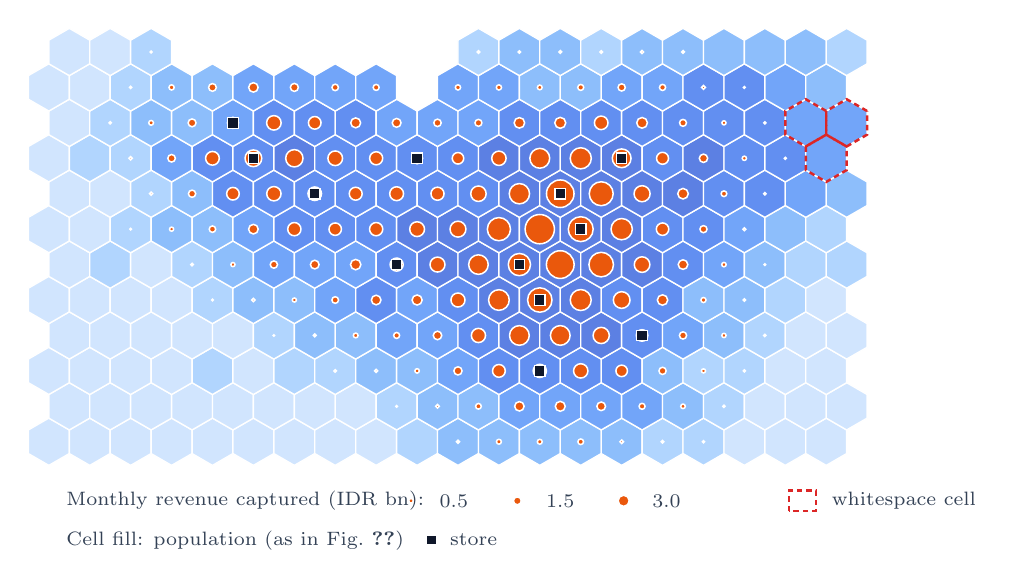
\begin{tikzpicture}
\fill[h3b200!72!white, draw=white, line width=0.5pt] (0.260,0.150) -- (0.000,0.300) -- (-0.260,0.150) -- (-0.260,-0.150) -- (-0.000,-0.300) -- (0.260,-0.150) -- cycle;
\fill[h3b200!72!white, draw=white, line width=0.5pt] (0.779,0.150) -- (0.520,0.300) -- (0.260,0.150) -- (0.260,-0.150) -- (0.520,-0.300) -- (0.779,-0.150) -- cycle;
\fill[h3b200!72!white, draw=white, line width=0.5pt] (1.299,0.150) -- (1.039,0.300) -- (0.779,0.150) -- (0.779,-0.150) -- (1.039,-0.300) -- (1.299,-0.150) -- cycle;
\fill[h3b200!72!white, draw=white, line width=0.5pt] (1.819,0.150) -- (1.559,0.300) -- (1.299,0.150) -- (1.299,-0.150) -- (1.559,-0.300) -- (1.819,-0.150) -- cycle;
\fill[h3b200!72!white, draw=white, line width=0.5pt] (2.338,0.150) -- (2.078,0.300) -- (1.819,0.150) -- (1.819,-0.150) -- (2.078,-0.300) -- (2.338,-0.150) -- cycle;
\fill[h3b200!72!white, draw=white, line width=0.5pt] (2.858,0.150) -- (2.598,0.300) -- (2.338,0.150) -- (2.338,-0.150) -- (2.598,-0.300) -- (2.858,-0.150) -- cycle;
\fill[h3b200!72!white, draw=white, line width=0.5pt] (3.377,0.150) -- (3.118,0.300) -- (2.858,0.150) -- (2.858,-0.150) -- (3.118,-0.300) -- (3.377,-0.150) -- cycle;
\fill[h3b200!72!white, draw=white, line width=0.5pt] (3.897,0.150) -- (3.637,0.300) -- (3.377,0.150) -- (3.377,-0.150) -- (3.637,-0.300) -- (3.897,-0.150) -- cycle;
\fill[h3b200!72!white, draw=white, line width=0.5pt] (4.417,0.150) -- (4.157,0.300) -- (3.897,0.150) -- (3.897,-0.150) -- (4.157,-0.300) -- (4.417,-0.150) -- cycle;
\fill[h3b300!72!white, draw=white, line width=0.5pt] (4.936,0.150) -- (4.677,0.300) -- (4.417,0.150) -- (4.417,-0.150) -- (4.677,-0.300) -- (4.936,-0.150) -- cycle;
\fill[h3b400!72!white, draw=white, line width=0.5pt] (5.456,0.150) -- (5.196,0.300) -- (4.936,0.150) -- (4.936,-0.150) -- (5.196,-0.300) -- (5.456,-0.150) -- cycle;
\fill[h3b400!72!white, draw=white, line width=0.5pt] (5.976,0.150) -- (5.716,0.300) -- (5.456,0.150) -- (5.456,-0.150) -- (5.716,-0.300) -- (5.976,-0.150) -- cycle;
\fill[h3b400!72!white, draw=white, line width=0.5pt] (6.495,0.150) -- (6.235,0.300) -- (5.976,0.150) -- (5.976,-0.150) -- (6.235,-0.300) -- (6.495,-0.150) -- cycle;
\fill[h3b400!72!white, draw=white, line width=0.5pt] (7.015,0.150) -- (6.755,0.300) -- (6.495,0.150) -- (6.495,-0.150) -- (6.755,-0.300) -- (7.015,-0.150) -- cycle;
\fill[h3b400!72!white, draw=white, line width=0.5pt] (7.534,0.150) -- (7.275,0.300) -- (7.015,0.150) -- (7.015,-0.150) -- (7.275,-0.300) -- (7.534,-0.150) -- cycle;
\fill[h3b300!72!white, draw=white, line width=0.5pt] (8.054,0.150) -- (7.794,0.300) -- (7.534,0.150) -- (7.534,-0.150) -- (7.794,-0.300) -- (8.054,-0.150) -- cycle;
\fill[h3b300!72!white, draw=white, line width=0.5pt] (8.574,0.150) -- (8.314,0.300) -- (8.054,0.150) -- (8.054,-0.150) -- (8.314,-0.300) -- (8.574,-0.150) -- cycle;
\fill[h3b200!72!white, draw=white, line width=0.5pt] (9.093,0.150) -- (8.833,0.300) -- (8.574,0.150) -- (8.574,-0.150) -- (8.833,-0.300) -- (9.093,-0.150) -- cycle;
\fill[h3b200!72!white, draw=white, line width=0.5pt] (9.613,0.150) -- (9.353,0.300) -- (9.093,0.150) -- (9.093,-0.150) -- (9.353,-0.300) -- (9.613,-0.150) -- cycle;
\fill[h3b200!72!white, draw=white, line width=0.5pt] (10.132,0.150) -- (9.873,0.300) -- (9.613,0.150) -- (9.613,-0.150) -- (9.873,-0.300) -- (10.132,-0.150) -- cycle;
\fill[h3b200!72!white, draw=white, line width=0.5pt] (0.520,0.600) -- (0.260,0.750) -- (-0.000,0.600) -- (0.000,0.300) -- (0.260,0.150) -- (0.520,0.300) -- cycle;
\fill[h3b200!72!white, draw=white, line width=0.5pt] (1.039,0.600) -- (0.779,0.750) -- (0.520,0.600) -- (0.520,0.300) -- (0.779,0.150) -- (1.039,0.300) -- cycle;
\fill[h3b200!72!white, draw=white, line width=0.5pt] (1.559,0.600) -- (1.299,0.750) -- (1.039,0.600) -- (1.039,0.300) -- (1.299,0.150) -- (1.559,0.300) -- cycle;
\fill[h3b200!72!white, draw=white, line width=0.5pt] (2.078,0.600) -- (1.819,0.750) -- (1.559,0.600) -- (1.559,0.300) -- (1.819,0.150) -- (2.078,0.300) -- cycle;
\fill[h3b200!72!white, draw=white, line width=0.5pt] (2.598,0.600) -- (2.338,0.750) -- (2.078,0.600) -- (2.078,0.300) -- (2.338,0.150) -- (2.598,0.300) -- cycle;
\fill[h3b200!72!white, draw=white, line width=0.5pt] (3.118,0.600) -- (2.858,0.750) -- (2.598,0.600) -- (2.598,0.300) -- (2.858,0.150) -- (3.118,0.300) -- cycle;
\fill[h3b200!72!white, draw=white, line width=0.5pt] (3.637,0.600) -- (3.377,0.750) -- (3.118,0.600) -- (3.118,0.300) -- (3.377,0.150) -- (3.637,0.300) -- cycle;
\fill[h3b200!72!white, draw=white, line width=0.5pt] (4.157,0.600) -- (3.897,0.750) -- (3.637,0.600) -- (3.637,0.300) -- (3.897,0.150) -- (4.157,0.300) -- cycle;
\fill[h3b300!72!white, draw=white, line width=0.5pt] (4.677,0.600) -- (4.417,0.750) -- (4.157,0.600) -- (4.157,0.300) -- (4.417,0.150) -- (4.677,0.300) -- cycle;
\fill[h3b400!72!white, draw=white, line width=0.5pt] (5.196,0.600) -- (4.936,0.750) -- (4.677,0.600) -- (4.677,0.300) -- (4.936,0.150) -- (5.196,0.300) -- cycle;
\fill[h3b400!72!white, draw=white, line width=0.5pt] (5.716,0.600) -- (5.456,0.750) -- (5.196,0.600) -- (5.196,0.300) -- (5.456,0.150) -- (5.716,0.300) -- cycle;
\fill[h3b500!72!white, draw=white, line width=0.5pt] (6.235,0.600) -- (5.976,0.750) -- (5.716,0.600) -- (5.716,0.300) -- (5.976,0.150) -- (6.235,0.300) -- cycle;
\fill[h3b500!72!white, draw=white, line width=0.5pt] (6.755,0.600) -- (6.495,0.750) -- (6.235,0.600) -- (6.235,0.300) -- (6.495,0.150) -- (6.755,0.300) -- cycle;
\fill[h3b500!72!white, draw=white, line width=0.5pt] (7.275,0.600) -- (7.015,0.750) -- (6.755,0.600) -- (6.755,0.300) -- (7.015,0.150) -- (7.275,0.300) -- cycle;
\fill[h3b500!72!white, draw=white, line width=0.5pt] (7.794,0.600) -- (7.534,0.750) -- (7.275,0.600) -- (7.275,0.300) -- (7.534,0.150) -- (7.794,0.300) -- cycle;
\fill[h3b400!72!white, draw=white, line width=0.5pt] (8.314,0.600) -- (8.054,0.750) -- (7.794,0.600) -- (7.794,0.300) -- (8.054,0.150) -- (8.314,0.300) -- cycle;
\fill[h3b300!72!white, draw=white, line width=0.5pt] (8.833,0.600) -- (8.574,0.750) -- (8.314,0.600) -- (8.314,0.300) -- (8.574,0.150) -- (8.833,0.300) -- cycle;
\fill[h3b200!72!white, draw=white, line width=0.5pt] (9.353,0.600) -- (9.093,0.750) -- (8.833,0.600) -- (8.833,0.300) -- (9.093,0.150) -- (9.353,0.300) -- cycle;
\fill[h3b200!72!white, draw=white, line width=0.5pt] (9.873,0.600) -- (9.613,0.750) -- (9.353,0.600) -- (9.353,0.300) -- (9.613,0.150) -- (9.873,0.300) -- cycle;
\fill[h3b200!72!white, draw=white, line width=0.5pt] (10.392,0.600) -- (10.132,0.750) -- (9.873,0.600) -- (9.873,0.300) -- (10.132,0.150) -- (10.392,0.300) -- cycle;
\fill[h3b200!72!white, draw=white, line width=0.5pt] (0.260,1.050) -- (0.000,1.200) -- (-0.260,1.050) -- (-0.260,0.750) -- (-0.000,0.600) -- (0.260,0.750) -- cycle;
\fill[h3b200!72!white, draw=white, line width=0.5pt] (0.779,1.050) -- (0.520,1.200) -- (0.260,1.050) -- (0.260,0.750) -- (0.520,0.600) -- (0.779,0.750) -- cycle;
\fill[h3b200!72!white, draw=white, line width=0.5pt] (1.299,1.050) -- (1.039,1.200) -- (0.779,1.050) -- (0.779,0.750) -- (1.039,0.600) -- (1.299,0.750) -- cycle;
\fill[h3b200!72!white, draw=white, line width=0.5pt] (1.819,1.050) -- (1.559,1.200) -- (1.299,1.050) -- (1.299,0.750) -- (1.559,0.600) -- (1.819,0.750) -- cycle;
\fill[h3b300!72!white, draw=white, line width=0.5pt] (2.338,1.050) -- (2.078,1.200) -- (1.819,1.050) -- (1.819,0.750) -- (2.078,0.600) -- (2.338,0.750) -- cycle;
\fill[h3b200!72!white, draw=white, line width=0.5pt] (2.858,1.050) -- (2.598,1.200) -- (2.338,1.050) -- (2.338,0.750) -- (2.598,0.600) -- (2.858,0.750) -- cycle;
\fill[h3b300!72!white, draw=white, line width=0.5pt] (3.377,1.050) -- (3.118,1.200) -- (2.858,1.050) -- (2.858,0.750) -- (3.118,0.600) -- (3.377,0.750) -- cycle;
\fill[h3b300!72!white, draw=white, line width=0.5pt] (3.897,1.050) -- (3.637,1.200) -- (3.377,1.050) -- (3.377,0.750) -- (3.637,0.600) -- (3.897,0.750) -- cycle;
\fill[h3b400!72!white, draw=white, line width=0.5pt] (4.417,1.050) -- (4.157,1.200) -- (3.897,1.050) -- (3.897,0.750) -- (4.157,0.600) -- (4.417,0.750) -- cycle;
\fill[h3b400!72!white, draw=white, line width=0.5pt] (4.936,1.050) -- (4.677,1.200) -- (4.417,1.050) -- (4.417,0.750) -- (4.677,0.600) -- (4.936,0.750) -- cycle;
\fill[h3b500!72!white, draw=white, line width=0.5pt] (5.456,1.050) -- (5.196,1.200) -- (4.936,1.050) -- (4.936,0.750) -- (5.196,0.600) -- (5.456,0.750) -- cycle;
\fill[h3b600!72!white, draw=white, line width=0.5pt] (5.976,1.050) -- (5.716,1.200) -- (5.456,1.050) -- (5.456,0.750) -- (5.716,0.600) -- (5.976,0.750) -- cycle;
\fill[h3b600!72!white, draw=white, line width=0.5pt] (6.495,1.050) -- (6.235,1.200) -- (5.976,1.050) -- (5.976,0.750) -- (6.235,0.600) -- (6.495,0.750) -- cycle;
\fill[h3b600!72!white, draw=white, line width=0.5pt] (7.015,1.050) -- (6.755,1.200) -- (6.495,1.050) -- (6.495,0.750) -- (6.755,0.600) -- (7.015,0.750) -- cycle;
\fill[h3b600!72!white, draw=white, line width=0.5pt] (7.534,1.050) -- (7.275,1.200) -- (7.015,1.050) -- (7.015,0.750) -- (7.275,0.600) -- (7.534,0.750) -- cycle;
\fill[h3b400!72!white, draw=white, line width=0.5pt] (8.054,1.050) -- (7.794,1.200) -- (7.534,1.050) -- (7.534,0.750) -- (7.794,0.600) -- (8.054,0.750) -- cycle;
\fill[h3b300!72!white, draw=white, line width=0.5pt] (8.574,1.050) -- (8.314,1.200) -- (8.054,1.050) -- (8.054,0.750) -- (8.314,0.600) -- (8.574,0.750) -- cycle;
\fill[h3b300!72!white, draw=white, line width=0.5pt] (9.093,1.050) -- (8.833,1.200) -- (8.574,1.050) -- (8.574,0.750) -- (8.833,0.600) -- (9.093,0.750) -- cycle;
\fill[h3b200!72!white, draw=white, line width=0.5pt] (9.613,1.050) -- (9.353,1.200) -- (9.093,1.050) -- (9.093,0.750) -- (9.353,0.600) -- (9.613,0.750) -- cycle;
\fill[h3b200!72!white, draw=white, line width=0.5pt] (10.132,1.050) -- (9.873,1.200) -- (9.613,1.050) -- (9.613,0.750) -- (9.873,0.600) -- (10.132,0.750) -- cycle;
\fill[h3b200!72!white, draw=white, line width=0.5pt] (0.520,1.500) -- (0.260,1.650) -- (-0.000,1.500) -- (0.000,1.200) -- (0.260,1.050) -- (0.520,1.200) -- cycle;
\fill[h3b200!72!white, draw=white, line width=0.5pt] (1.039,1.500) -- (0.779,1.650) -- (0.520,1.500) -- (0.520,1.200) -- (0.779,1.050) -- (1.039,1.200) -- cycle;
\fill[h3b200!72!white, draw=white, line width=0.5pt] (1.559,1.500) -- (1.299,1.650) -- (1.039,1.500) -- (1.039,1.200) -- (1.299,1.050) -- (1.559,1.200) -- cycle;
\fill[h3b200!72!white, draw=white, line width=0.5pt] (2.078,1.500) -- (1.819,1.650) -- (1.559,1.500) -- (1.559,1.200) -- (1.819,1.050) -- (2.078,1.200) -- cycle;
\fill[h3b200!72!white, draw=white, line width=0.5pt] (2.598,1.500) -- (2.338,1.650) -- (2.078,1.500) -- (2.078,1.200) -- (2.338,1.050) -- (2.598,1.200) -- cycle;
\fill[h3b300!72!white, draw=white, line width=0.5pt] (3.118,1.500) -- (2.858,1.650) -- (2.598,1.500) -- (2.598,1.200) -- (2.858,1.050) -- (3.118,1.200) -- cycle;
\fill[h3b400!72!white, draw=white, line width=0.5pt] (3.637,1.500) -- (3.377,1.650) -- (3.118,1.500) -- (3.118,1.200) -- (3.377,1.050) -- (3.637,1.200) -- cycle;
\fill[h3b400!72!white, draw=white, line width=0.5pt] (4.157,1.500) -- (3.897,1.650) -- (3.637,1.500) -- (3.637,1.200) -- (3.897,1.050) -- (4.157,1.200) -- cycle;
\fill[h3b500!72!white, draw=white, line width=0.5pt] (4.677,1.500) -- (4.417,1.650) -- (4.157,1.500) -- (4.157,1.200) -- (4.417,1.050) -- (4.677,1.200) -- cycle;
\fill[h3b500!72!white, draw=white, line width=0.5pt] (5.196,1.500) -- (4.936,1.650) -- (4.677,1.500) -- (4.677,1.200) -- (4.936,1.050) -- (5.196,1.200) -- cycle;
\fill[h3b600!72!white, draw=white, line width=0.5pt] (5.716,1.500) -- (5.456,1.650) -- (5.196,1.500) -- (5.196,1.200) -- (5.456,1.050) -- (5.716,1.200) -- cycle;
\fill[h3b700!72!white, draw=white, line width=0.5pt] (6.235,1.500) -- (5.976,1.650) -- (5.716,1.500) -- (5.716,1.200) -- (5.976,1.050) -- (6.235,1.200) -- cycle;
\fill[h3b700!72!white, draw=white, line width=0.5pt] (6.755,1.500) -- (6.495,1.650) -- (6.235,1.500) -- (6.235,1.200) -- (6.495,1.050) -- (6.755,1.200) -- cycle;
\fill[h3b700!72!white, draw=white, line width=0.5pt] (7.275,1.500) -- (7.015,1.650) -- (6.755,1.500) -- (6.755,1.200) -- (7.015,1.050) -- (7.275,1.200) -- cycle;
\fill[h3b600!72!white, draw=white, line width=0.5pt] (7.794,1.500) -- (7.534,1.650) -- (7.275,1.500) -- (7.275,1.200) -- (7.534,1.050) -- (7.794,1.200) -- cycle;
\fill[h3b500!72!white, draw=white, line width=0.5pt] (8.314,1.500) -- (8.054,1.650) -- (7.794,1.500) -- (7.794,1.200) -- (8.054,1.050) -- (8.314,1.200) -- cycle;
\fill[h3b400!72!white, draw=white, line width=0.5pt] (8.833,1.500) -- (8.574,1.650) -- (8.314,1.500) -- (8.314,1.200) -- (8.574,1.050) -- (8.833,1.200) -- cycle;
\fill[h3b300!72!white, draw=white, line width=0.5pt] (9.353,1.500) -- (9.093,1.650) -- (8.833,1.500) -- (8.833,1.200) -- (9.093,1.050) -- (9.353,1.200) -- cycle;
\fill[h3b200!72!white, draw=white, line width=0.5pt] (9.873,1.500) -- (9.613,1.650) -- (9.353,1.500) -- (9.353,1.200) -- (9.613,1.050) -- (9.873,1.200) -- cycle;
\fill[h3b200!72!white, draw=white, line width=0.5pt] (10.392,1.500) -- (10.132,1.650) -- (9.873,1.500) -- (9.873,1.200) -- (10.132,1.050) -- (10.392,1.200) -- cycle;
\fill[h3b200!72!white, draw=white, line width=0.5pt] (0.260,1.950) -- (0.000,2.100) -- (-0.260,1.950) -- (-0.260,1.650) -- (-0.000,1.500) -- (0.260,1.650) -- cycle;
\fill[h3b200!72!white, draw=white, line width=0.5pt] (0.779,1.950) -- (0.520,2.100) -- (0.260,1.950) -- (0.260,1.650) -- (0.520,1.500) -- (0.779,1.650) -- cycle;
\fill[h3b200!72!white, draw=white, line width=0.5pt] (1.299,1.950) -- (1.039,2.100) -- (0.779,1.950) -- (0.779,1.650) -- (1.039,1.500) -- (1.299,1.650) -- cycle;
\fill[h3b200!72!white, draw=white, line width=0.5pt] (1.819,1.950) -- (1.559,2.100) -- (1.299,1.950) -- (1.299,1.650) -- (1.559,1.500) -- (1.819,1.650) -- cycle;
\fill[h3b300!72!white, draw=white, line width=0.5pt] (2.338,1.950) -- (2.078,2.100) -- (1.819,1.950) -- (1.819,1.650) -- (2.078,1.500) -- (2.338,1.650) -- cycle;
\fill[h3b400!72!white, draw=white, line width=0.5pt] (2.858,1.950) -- (2.598,2.100) -- (2.338,1.950) -- (2.338,1.650) -- (2.598,1.500) -- (2.858,1.650) -- cycle;
\fill[h3b400!72!white, draw=white, line width=0.5pt] (3.377,1.950) -- (3.118,2.100) -- (2.858,1.950) -- (2.858,1.650) -- (3.118,1.500) -- (3.377,1.650) -- cycle;
\fill[h3b500!72!white, draw=white, line width=0.5pt] (3.897,1.950) -- (3.637,2.100) -- (3.377,1.950) -- (3.377,1.650) -- (3.637,1.500) -- (3.897,1.650) -- cycle;
\fill[h3b600!72!white, draw=white, line width=0.5pt] (4.417,1.950) -- (4.157,2.100) -- (3.897,1.950) -- (3.897,1.650) -- (4.157,1.500) -- (4.417,1.650) -- cycle;
\fill[h3b500!72!white, draw=white, line width=0.5pt] (4.936,1.950) -- (4.677,2.100) -- (4.417,1.950) -- (4.417,1.650) -- (4.677,1.500) -- (4.936,1.650) -- cycle;
\fill[h3b600!72!white, draw=white, line width=0.5pt] (5.456,1.950) -- (5.196,2.100) -- (4.936,1.950) -- (4.936,1.650) -- (5.196,1.500) -- (5.456,1.650) -- cycle;
\fill[h3b700!72!white, draw=white, line width=0.5pt] (5.976,1.950) -- (5.716,2.100) -- (5.456,1.950) -- (5.456,1.650) -- (5.716,1.500) -- (5.976,1.650) -- cycle;
\fill[h3b700!72!white, draw=white, line width=0.5pt] (6.495,1.950) -- (6.235,2.100) -- (5.976,1.950) -- (5.976,1.650) -- (6.235,1.500) -- (6.495,1.650) -- cycle;
\fill[h3b700!72!white, draw=white, line width=0.5pt] (7.015,1.950) -- (6.755,2.100) -- (6.495,1.950) -- (6.495,1.650) -- (6.755,1.500) -- (7.015,1.650) -- cycle;
\fill[h3b600!72!white, draw=white, line width=0.5pt] (7.534,1.950) -- (7.275,2.100) -- (7.015,1.950) -- (7.015,1.650) -- (7.275,1.500) -- (7.534,1.650) -- cycle;
\fill[h3b600!72!white, draw=white, line width=0.5pt] (8.054,1.950) -- (7.794,2.100) -- (7.534,1.950) -- (7.534,1.650) -- (7.794,1.500) -- (8.054,1.650) -- cycle;
\fill[h3b400!72!white, draw=white, line width=0.5pt] (8.574,1.950) -- (8.314,2.100) -- (8.054,1.950) -- (8.054,1.650) -- (8.314,1.500) -- (8.574,1.650) -- cycle;
\fill[h3b400!72!white, draw=white, line width=0.5pt] (9.093,1.950) -- (8.833,2.100) -- (8.574,1.950) -- (8.574,1.650) -- (8.833,1.500) -- (9.093,1.650) -- cycle;
\fill[h3b300!72!white, draw=white, line width=0.5pt] (9.613,1.950) -- (9.353,2.100) -- (9.093,1.950) -- (9.093,1.650) -- (9.353,1.500) -- (9.613,1.650) -- cycle;
\fill[h3b200!72!white, draw=white, line width=0.5pt] (10.132,1.950) -- (9.873,2.100) -- (9.613,1.950) -- (9.613,1.650) -- (9.873,1.500) -- (10.132,1.650) -- cycle;
\fill[h3b200!72!white, draw=white, line width=0.5pt] (0.520,2.400) -- (0.260,2.550) -- (-0.000,2.400) -- (0.000,2.100) -- (0.260,1.950) -- (0.520,2.100) -- cycle;
\fill[h3b300!72!white, draw=white, line width=0.5pt] (1.039,2.400) -- (0.779,2.550) -- (0.520,2.400) -- (0.520,2.100) -- (0.779,1.950) -- (1.039,2.100) -- cycle;
\fill[h3b200!72!white, draw=white, line width=0.5pt] (1.559,2.400) -- (1.299,2.550) -- (1.039,2.400) -- (1.039,2.100) -- (1.299,1.950) -- (1.559,2.100) -- cycle;
\fill[h3b300!72!white, draw=white, line width=0.5pt] (2.078,2.400) -- (1.819,2.550) -- (1.559,2.400) -- (1.559,2.100) -- (1.819,1.950) -- (2.078,2.100) -- cycle;
\fill[h3b400!72!white, draw=white, line width=0.5pt] (2.598,2.400) -- (2.338,2.550) -- (2.078,2.400) -- (2.078,2.100) -- (2.338,1.950) -- (2.598,2.100) -- cycle;
\fill[h3b500!72!white, draw=white, line width=0.5pt] (3.118,2.400) -- (2.858,2.550) -- (2.598,2.400) -- (2.598,2.100) -- (2.858,1.950) -- (3.118,2.100) -- cycle;
\fill[h3b500!72!white, draw=white, line width=0.5pt] (3.637,2.400) -- (3.377,2.550) -- (3.118,2.400) -- (3.118,2.100) -- (3.377,1.950) -- (3.637,2.100) -- cycle;
\fill[h3b500!72!white, draw=white, line width=0.5pt] (4.157,2.400) -- (3.897,2.550) -- (3.637,2.400) -- (3.637,2.100) -- (3.897,1.950) -- (4.157,2.100) -- cycle;
\fill[h3b600!72!white, draw=white, line width=0.5pt] (4.677,2.400) -- (4.417,2.550) -- (4.157,2.400) -- (4.157,2.100) -- (4.417,1.950) -- (4.677,2.100) -- cycle;
\fill[h3b700!72!white, draw=white, line width=0.5pt] (5.196,2.400) -- (4.936,2.550) -- (4.677,2.400) -- (4.677,2.100) -- (4.936,1.950) -- (5.196,2.100) -- cycle;
\fill[h3b700!72!white, draw=white, line width=0.5pt] (5.716,2.400) -- (5.456,2.550) -- (5.196,2.400) -- (5.196,2.100) -- (5.456,1.950) -- (5.716,2.100) -- cycle;
\fill[h3b700!72!white, draw=white, line width=0.5pt] (6.235,2.400) -- (5.976,2.550) -- (5.716,2.400) -- (5.716,2.100) -- (5.976,1.950) -- (6.235,2.100) -- cycle;
\fill[h3b700!72!white, draw=white, line width=0.5pt] (6.755,2.400) -- (6.495,2.550) -- (6.235,2.400) -- (6.235,2.100) -- (6.495,1.950) -- (6.755,2.100) -- cycle;
\fill[h3b700!72!white, draw=white, line width=0.5pt] (7.275,2.400) -- (7.015,2.550) -- (6.755,2.400) -- (6.755,2.100) -- (7.015,1.950) -- (7.275,2.100) -- cycle;
\fill[h3b700!72!white, draw=white, line width=0.5pt] (7.794,2.400) -- (7.534,2.550) -- (7.275,2.400) -- (7.275,2.100) -- (7.534,1.950) -- (7.794,2.100) -- cycle;
\fill[h3b600!72!white, draw=white, line width=0.5pt] (8.314,2.400) -- (8.054,2.550) -- (7.794,2.400) -- (7.794,2.100) -- (8.054,1.950) -- (8.314,2.100) -- cycle;
\fill[h3b500!72!white, draw=white, line width=0.5pt] (8.833,2.400) -- (8.574,2.550) -- (8.314,2.400) -- (8.314,2.100) -- (8.574,1.950) -- (8.833,2.100) -- cycle;
\fill[h3b400!72!white, draw=white, line width=0.5pt] (9.353,2.400) -- (9.093,2.550) -- (8.833,2.400) -- (8.833,2.100) -- (9.093,1.950) -- (9.353,2.100) -- cycle;
\fill[h3b300!72!white, draw=white, line width=0.5pt] (9.873,2.400) -- (9.613,2.550) -- (9.353,2.400) -- (9.353,2.100) -- (9.613,1.950) -- (9.873,2.100) -- cycle;
\fill[h3b300!72!white, draw=white, line width=0.5pt] (10.392,2.400) -- (10.132,2.550) -- (9.873,2.400) -- (9.873,2.100) -- (10.132,1.950) -- (10.392,2.100) -- cycle;
\fill[h3b200!72!white, draw=white, line width=0.5pt] (0.260,2.850) -- (0.000,3.000) -- (-0.260,2.850) -- (-0.260,2.550) -- (-0.000,2.400) -- (0.260,2.550) -- cycle;
\fill[h3b200!72!white, draw=white, line width=0.5pt] (0.779,2.850) -- (0.520,3.000) -- (0.260,2.850) -- (0.260,2.550) -- (0.520,2.400) -- (0.779,2.550) -- cycle;
\fill[h3b300!72!white, draw=white, line width=0.5pt] (1.299,2.850) -- (1.039,3.000) -- (0.779,2.850) -- (0.779,2.550) -- (1.039,2.400) -- (1.299,2.550) -- cycle;
\fill[h3b400!72!white, draw=white, line width=0.5pt] (1.819,2.850) -- (1.559,3.000) -- (1.299,2.850) -- (1.299,2.550) -- (1.559,2.400) -- (1.819,2.550) -- cycle;
\fill[h3b400!72!white, draw=white, line width=0.5pt] (2.338,2.850) -- (2.078,3.000) -- (1.819,2.850) -- (1.819,2.550) -- (2.078,2.400) -- (2.338,2.550) -- cycle;
\fill[h3b500!72!white, draw=white, line width=0.5pt] (2.858,2.850) -- (2.598,3.000) -- (2.338,2.850) -- (2.338,2.550) -- (2.598,2.400) -- (2.858,2.550) -- cycle;
\fill[h3b600!72!white, draw=white, line width=0.5pt] (3.377,2.850) -- (3.118,3.000) -- (2.858,2.850) -- (2.858,2.550) -- (3.118,2.400) -- (3.377,2.550) -- cycle;
\fill[h3b600!72!white, draw=white, line width=0.5pt] (3.897,2.850) -- (3.637,3.000) -- (3.377,2.850) -- (3.377,2.550) -- (3.637,2.400) -- (3.897,2.550) -- cycle;
\fill[h3b600!72!white, draw=white, line width=0.5pt] (4.417,2.850) -- (4.157,3.000) -- (3.897,2.850) -- (3.897,2.550) -- (4.157,2.400) -- (4.417,2.550) -- cycle;
\fill[h3b700!72!white, draw=white, line width=0.5pt] (4.936,2.850) -- (4.677,3.000) -- (4.417,2.850) -- (4.417,2.550) -- (4.677,2.400) -- (4.936,2.550) -- cycle;
\fill[h3b700!72!white, draw=white, line width=0.5pt] (5.456,2.850) -- (5.196,3.000) -- (4.936,2.850) -- (4.936,2.550) -- (5.196,2.400) -- (5.456,2.550) -- cycle;
\fill[h3b700!72!white, draw=white, line width=0.5pt] (5.976,2.850) -- (5.716,3.000) -- (5.456,2.850) -- (5.456,2.550) -- (5.716,2.400) -- (5.976,2.550) -- cycle;
\fill[h3b700!72!white, draw=white, line width=0.5pt] (6.495,2.850) -- (6.235,3.000) -- (5.976,2.850) -- (5.976,2.550) -- (6.235,2.400) -- (6.495,2.550) -- cycle;
\fill[h3b700!72!white, draw=white, line width=0.5pt] (7.015,2.850) -- (6.755,3.000) -- (6.495,2.850) -- (6.495,2.550) -- (6.755,2.400) -- (7.015,2.550) -- cycle;
\fill[h3b700!72!white, draw=white, line width=0.5pt] (7.534,2.850) -- (7.275,3.000) -- (7.015,2.850) -- (7.015,2.550) -- (7.275,2.400) -- (7.534,2.550) -- cycle;
\fill[h3b600!72!white, draw=white, line width=0.5pt] (8.054,2.850) -- (7.794,3.000) -- (7.534,2.850) -- (7.534,2.550) -- (7.794,2.400) -- (8.054,2.550) -- cycle;
\fill[h3b600!72!white, draw=white, line width=0.5pt] (8.574,2.850) -- (8.314,3.000) -- (8.054,2.850) -- (8.054,2.550) -- (8.314,2.400) -- (8.574,2.550) -- cycle;
\fill[h3b500!72!white, draw=white, line width=0.5pt] (9.093,2.850) -- (8.833,3.000) -- (8.574,2.850) -- (8.574,2.550) -- (8.833,2.400) -- (9.093,2.550) -- cycle;
\fill[h3b400!72!white, draw=white, line width=0.5pt] (9.613,2.850) -- (9.353,3.000) -- (9.093,2.850) -- (9.093,2.550) -- (9.353,2.400) -- (9.613,2.550) -- cycle;
\fill[h3b300!72!white, draw=white, line width=0.5pt] (10.132,2.850) -- (9.873,3.000) -- (9.613,2.850) -- (9.613,2.550) -- (9.873,2.400) -- (10.132,2.550) -- cycle;
\fill[h3b200!72!white, draw=white, line width=0.5pt] (0.520,3.300) -- (0.260,3.450) -- (-0.000,3.300) -- (0.000,3.000) -- (0.260,2.850) -- (0.520,3.000) -- cycle;
\fill[h3b200!72!white, draw=white, line width=0.5pt] (1.039,3.300) -- (0.779,3.450) -- (0.520,3.300) -- (0.520,3.000) -- (0.779,2.850) -- (1.039,3.000) -- cycle;
\fill[h3b300!72!white, draw=white, line width=0.5pt] (1.559,3.300) -- (1.299,3.450) -- (1.039,3.300) -- (1.039,3.000) -- (1.299,2.850) -- (1.559,3.000) -- cycle;
\fill[h3b400!72!white, draw=white, line width=0.5pt] (2.078,3.300) -- (1.819,3.450) -- (1.559,3.300) -- (1.559,3.000) -- (1.819,2.850) -- (2.078,3.000) -- cycle;
\fill[h3b600!72!white, draw=white, line width=0.5pt] (2.598,3.300) -- (2.338,3.450) -- (2.078,3.300) -- (2.078,3.000) -- (2.338,2.850) -- (2.598,3.000) -- cycle;
\fill[h3b600!72!white, draw=white, line width=0.5pt] (3.118,3.300) -- (2.858,3.450) -- (2.598,3.300) -- (2.598,3.000) -- (2.858,2.850) -- (3.118,3.000) -- cycle;
\fill[h3b600!72!white, draw=white, line width=0.5pt] (3.637,3.300) -- (3.377,3.450) -- (3.118,3.300) -- (3.118,3.000) -- (3.377,2.850) -- (3.637,3.000) -- cycle;
\fill[h3b600!72!white, draw=white, line width=0.5pt] (4.157,3.300) -- (3.897,3.450) -- (3.637,3.300) -- (3.637,3.000) -- (3.897,2.850) -- (4.157,3.000) -- cycle;
\fill[h3b600!72!white, draw=white, line width=0.5pt] (4.677,3.300) -- (4.417,3.450) -- (4.157,3.300) -- (4.157,3.000) -- (4.417,2.850) -- (4.677,3.000) -- cycle;
\fill[h3b600!72!white, draw=white, line width=0.5pt] (5.196,3.300) -- (4.936,3.450) -- (4.677,3.300) -- (4.677,3.000) -- (4.936,2.850) -- (5.196,3.000) -- cycle;
\fill[h3b600!72!white, draw=white, line width=0.5pt] (5.716,3.300) -- (5.456,3.450) -- (5.196,3.300) -- (5.196,3.000) -- (5.456,2.850) -- (5.716,3.000) -- cycle;
\fill[h3b700!72!white, draw=white, line width=0.5pt] (6.235,3.300) -- (5.976,3.450) -- (5.716,3.300) -- (5.716,3.000) -- (5.976,2.850) -- (6.235,3.000) -- cycle;
\fill[h3b700!72!white, draw=white, line width=0.5pt] (6.755,3.300) -- (6.495,3.450) -- (6.235,3.300) -- (6.235,3.000) -- (6.495,2.850) -- (6.755,3.000) -- cycle;
\fill[h3b700!72!white, draw=white, line width=0.5pt] (7.275,3.300) -- (7.015,3.450) -- (6.755,3.300) -- (6.755,3.000) -- (7.015,2.850) -- (7.275,3.000) -- cycle;
\fill[h3b700!72!white, draw=white, line width=0.5pt] (7.794,3.300) -- (7.534,3.450) -- (7.275,3.300) -- (7.275,3.000) -- (7.534,2.850) -- (7.794,3.000) -- cycle;
\fill[h3b700!72!white, draw=white, line width=0.5pt] (8.314,3.300) -- (8.054,3.450) -- (7.794,3.300) -- (7.794,3.000) -- (8.054,2.850) -- (8.314,3.000) -- cycle;
\fill[h3b600!72!white, draw=white, line width=0.5pt] (8.833,3.300) -- (8.574,3.450) -- (8.314,3.300) -- (8.314,3.000) -- (8.574,2.850) -- (8.833,3.000) -- cycle;
\fill[h3b600!72!white, draw=white, line width=0.5pt] (9.353,3.300) -- (9.093,3.450) -- (8.833,3.300) -- (8.833,3.000) -- (9.093,2.850) -- (9.353,3.000) -- cycle;
\fill[h3b500!72!white, draw=white, line width=0.5pt] (9.873,3.300) -- (9.613,3.450) -- (9.353,3.300) -- (9.353,3.000) -- (9.613,2.850) -- (9.873,3.000) -- cycle;
\fill[h3b400!72!white, draw=white, line width=0.5pt] (10.392,3.300) -- (10.132,3.450) -- (9.873,3.300) -- (9.873,3.000) -- (10.132,2.850) -- (10.392,3.000) -- cycle;
\fill[h3b200!72!white, draw=white, line width=0.5pt] (0.260,3.750) -- (0.000,3.900) -- (-0.260,3.750) -- (-0.260,3.450) -- (-0.000,3.300) -- (0.260,3.450) -- cycle;
\fill[h3b300!72!white, draw=white, line width=0.5pt] (0.779,3.750) -- (0.520,3.900) -- (0.260,3.750) -- (0.260,3.450) -- (0.520,3.300) -- (0.779,3.450) -- cycle;
\fill[h3b300!72!white, draw=white, line width=0.5pt] (1.299,3.750) -- (1.039,3.900) -- (0.779,3.750) -- (0.779,3.450) -- (1.039,3.300) -- (1.299,3.450) -- cycle;
\fill[h3b500!72!white, draw=white, line width=0.5pt] (1.819,3.750) -- (1.559,3.900) -- (1.299,3.750) -- (1.299,3.450) -- (1.559,3.300) -- (1.819,3.450) -- cycle;
\fill[h3b600!72!white, draw=white, line width=0.5pt] (2.338,3.750) -- (2.078,3.900) -- (1.819,3.750) -- (1.819,3.450) -- (2.078,3.300) -- (2.338,3.450) -- cycle;
\fill[h3b600!72!white, draw=white, line width=0.5pt] (2.858,3.750) -- (2.598,3.900) -- (2.338,3.750) -- (2.338,3.450) -- (2.598,3.300) -- (2.858,3.450) -- cycle;
\fill[h3b700!72!white, draw=white, line width=0.5pt] (3.377,3.750) -- (3.118,3.900) -- (2.858,3.750) -- (2.858,3.450) -- (3.118,3.300) -- (3.377,3.450) -- cycle;
\fill[h3b600!72!white, draw=white, line width=0.5pt] (3.897,3.750) -- (3.637,3.900) -- (3.377,3.750) -- (3.377,3.450) -- (3.637,3.300) -- (3.897,3.450) -- cycle;
\fill[h3b600!72!white, draw=white, line width=0.5pt] (4.417,3.750) -- (4.157,3.900) -- (3.897,3.750) -- (3.897,3.450) -- (4.157,3.300) -- (4.417,3.450) -- cycle;
\fill[h3b600!72!white, draw=white, line width=0.5pt] (4.936,3.750) -- (4.677,3.900) -- (4.417,3.750) -- (4.417,3.450) -- (4.677,3.300) -- (4.936,3.450) -- cycle;
\fill[h3b600!72!white, draw=white, line width=0.5pt] (5.456,3.750) -- (5.196,3.900) -- (4.936,3.750) -- (4.936,3.450) -- (5.196,3.300) -- (5.456,3.450) -- cycle;
\fill[h3b700!72!white, draw=white, line width=0.5pt] (5.976,3.750) -- (5.716,3.900) -- (5.456,3.750) -- (5.456,3.450) -- (5.716,3.300) -- (5.976,3.450) -- cycle;
\fill[h3b700!72!white, draw=white, line width=0.5pt] (6.495,3.750) -- (6.235,3.900) -- (5.976,3.750) -- (5.976,3.450) -- (6.235,3.300) -- (6.495,3.450) -- cycle;
\fill[h3b700!72!white, draw=white, line width=0.5pt] (7.015,3.750) -- (6.755,3.900) -- (6.495,3.750) -- (6.495,3.450) -- (6.755,3.300) -- (7.015,3.450) -- cycle;
\fill[h3b700!72!white, draw=white, line width=0.5pt] (7.534,3.750) -- (7.275,3.900) -- (7.015,3.750) -- (7.015,3.450) -- (7.275,3.300) -- (7.534,3.450) -- cycle;
\fill[h3b600!72!white, draw=white, line width=0.5pt] (8.054,3.750) -- (7.794,3.900) -- (7.534,3.750) -- (7.534,3.450) -- (7.794,3.300) -- (8.054,3.450) -- cycle;
\fill[h3b700!72!white, draw=white, line width=0.5pt] (8.574,3.750) -- (8.314,3.900) -- (8.054,3.750) -- (8.054,3.450) -- (8.314,3.300) -- (8.574,3.450) -- cycle;
\fill[h3b600!72!white, draw=white, line width=0.5pt] (9.093,3.750) -- (8.833,3.900) -- (8.574,3.750) -- (8.574,3.450) -- (8.833,3.300) -- (9.093,3.450) -- cycle;
\fill[h3b600!72!white, draw=white, line width=0.5pt] (9.613,3.750) -- (9.353,3.900) -- (9.093,3.750) -- (9.093,3.450) -- (9.353,3.300) -- (9.613,3.450) -- cycle;
\fill[h3b500!72!white, draw=white, line width=0.5pt] (10.132,3.750) -- (9.873,3.900) -- (9.613,3.750) -- (9.613,3.450) -- (9.873,3.300) -- (10.132,3.450) -- cycle;
\fill[h3b200!72!white, draw=white, line width=0.5pt] (0.520,4.200) -- (0.260,4.350) -- (-0.000,4.200) -- (0.000,3.900) -- (0.260,3.750) -- (0.520,3.900) -- cycle;
\fill[h3b300!72!white, draw=white, line width=0.5pt] (1.039,4.200) -- (0.779,4.350) -- (0.520,4.200) -- (0.520,3.900) -- (0.779,3.750) -- (1.039,3.900) -- cycle;
\fill[h3b400!72!white, draw=white, line width=0.5pt] (1.559,4.200) -- (1.299,4.350) -- (1.039,4.200) -- (1.039,3.900) -- (1.299,3.750) -- (1.559,3.900) -- cycle;
\fill[h3b400!72!white, draw=white, line width=0.5pt] (2.078,4.200) -- (1.819,4.350) -- (1.559,4.200) -- (1.559,3.900) -- (1.819,3.750) -- (2.078,3.900) -- cycle;
\fill[h3b500!72!white, draw=white, line width=0.5pt] (2.598,4.200) -- (2.338,4.350) -- (2.078,4.200) -- (2.078,3.900) -- (2.338,3.750) -- (2.598,3.900) -- cycle;
\fill[h3b600!72!white, draw=white, line width=0.5pt] (3.118,4.200) -- (2.858,4.350) -- (2.598,4.200) -- (2.598,3.900) -- (2.858,3.750) -- (3.118,3.900) -- cycle;
\fill[h3b600!72!white, draw=white, line width=0.5pt] (3.637,4.200) -- (3.377,4.350) -- (3.118,4.200) -- (3.118,3.900) -- (3.377,3.750) -- (3.637,3.900) -- cycle;
\fill[h3b600!72!white, draw=white, line width=0.5pt] (4.157,4.200) -- (3.897,4.350) -- (3.637,4.200) -- (3.637,3.900) -- (3.897,3.750) -- (4.157,3.900) -- cycle;
\fill[h3b500!72!white, draw=white, line width=0.5pt] (4.677,4.200) -- (4.417,4.350) -- (4.157,4.200) -- (4.157,3.900) -- (4.417,3.750) -- (4.677,3.900) -- cycle;
\fill[h3b500!72!white, draw=white, line width=0.5pt] (5.196,4.200) -- (4.936,4.350) -- (4.677,4.200) -- (4.677,3.900) -- (4.936,3.750) -- (5.196,3.900) -- cycle;
\fill[h3b500!72!white, draw=white, line width=0.5pt] (5.716,4.200) -- (5.456,4.350) -- (5.196,4.200) -- (5.196,3.900) -- (5.456,3.750) -- (5.716,3.900) -- cycle;
\fill[h3b600!72!white, draw=white, line width=0.5pt] (6.235,4.200) -- (5.976,4.350) -- (5.716,4.200) -- (5.716,3.900) -- (5.976,3.750) -- (6.235,3.900) -- cycle;
\fill[h3b600!72!white, draw=white, line width=0.5pt] (6.755,4.200) -- (6.495,4.350) -- (6.235,4.200) -- (6.235,3.900) -- (6.495,3.750) -- (6.755,3.900) -- cycle;
\fill[h3b600!72!white, draw=white, line width=0.5pt] (7.275,4.200) -- (7.015,4.350) -- (6.755,4.200) -- (6.755,3.900) -- (7.015,3.750) -- (7.275,3.900) -- cycle;
\fill[h3b600!72!white, draw=white, line width=0.5pt] (7.794,4.200) -- (7.534,4.350) -- (7.275,4.200) -- (7.275,3.900) -- (7.534,3.750) -- (7.794,3.900) -- cycle;
\fill[h3b600!72!white, draw=white, line width=0.5pt] (8.314,4.200) -- (8.054,4.350) -- (7.794,4.200) -- (7.794,3.900) -- (8.054,3.750) -- (8.314,3.900) -- cycle;
\fill[h3b600!72!white, draw=white, line width=0.5pt] (8.833,4.200) -- (8.574,4.350) -- (8.314,4.200) -- (8.314,3.900) -- (8.574,3.750) -- (8.833,3.900) -- cycle;
\fill[h3b600!72!white, draw=white, line width=0.5pt] (9.353,4.200) -- (9.093,4.350) -- (8.833,4.200) -- (8.833,3.900) -- (9.093,3.750) -- (9.353,3.900) -- cycle;
\fill[h3b500!72!white, draw=white, line width=0.5pt] (9.873,4.200) -- (9.613,4.350) -- (9.353,4.200) -- (9.353,3.900) -- (9.613,3.750) -- (9.873,3.900) -- cycle;
\fill[h3b500!72!white, draw=white, line width=0.5pt] (10.392,4.200) -- (10.132,4.350) -- (9.873,4.200) -- (9.873,3.900) -- (10.132,3.750) -- (10.392,3.900) -- cycle;
\fill[h3b200!72!white, draw=white, line width=0.5pt] (0.260,4.650) -- (0.000,4.800) -- (-0.260,4.650) -- (-0.260,4.350) -- (-0.000,4.200) -- (0.260,4.350) -- cycle;
\fill[h3b200!72!white, draw=white, line width=0.5pt] (0.779,4.650) -- (0.520,4.800) -- (0.260,4.650) -- (0.260,4.350) -- (0.520,4.200) -- (0.779,4.350) -- cycle;
\fill[h3b300!72!white, draw=white, line width=0.5pt] (1.299,4.650) -- (1.039,4.800) -- (0.779,4.650) -- (0.779,4.350) -- (1.039,4.200) -- (1.299,4.350) -- cycle;
\fill[h3b400!72!white, draw=white, line width=0.5pt] (1.819,4.650) -- (1.559,4.800) -- (1.299,4.650) -- (1.299,4.350) -- (1.559,4.200) -- (1.819,4.350) -- cycle;
\fill[h3b400!72!white, draw=white, line width=0.5pt] (2.338,4.650) -- (2.078,4.800) -- (1.819,4.650) -- (1.819,4.350) -- (2.078,4.200) -- (2.338,4.350) -- cycle;
\fill[h3b500!72!white, draw=white, line width=0.5pt] (2.858,4.650) -- (2.598,4.800) -- (2.338,4.650) -- (2.338,4.350) -- (2.598,4.200) -- (2.858,4.350) -- cycle;
\fill[h3b500!72!white, draw=white, line width=0.5pt] (3.377,4.650) -- (3.118,4.800) -- (2.858,4.650) -- (2.858,4.350) -- (3.118,4.200) -- (3.377,4.350) -- cycle;
\fill[h3b500!72!white, draw=white, line width=0.5pt] (3.897,4.650) -- (3.637,4.800) -- (3.377,4.650) -- (3.377,4.350) -- (3.637,4.200) -- (3.897,4.350) -- cycle;
\fill[h3b500!72!white, draw=white, line width=0.5pt] (4.417,4.650) -- (4.157,4.800) -- (3.897,4.650) -- (3.897,4.350) -- (4.157,4.200) -- (4.417,4.350) -- cycle;
\fill[h3b500!72!white, draw=white, line width=0.5pt] (5.456,4.650) -- (5.196,4.800) -- (4.936,4.650) -- (4.936,4.350) -- (5.196,4.200) -- (5.456,4.350) -- cycle;
\fill[h3b500!72!white, draw=white, line width=0.5pt] (5.976,4.650) -- (5.716,4.800) -- (5.456,4.650) -- (5.456,4.350) -- (5.716,4.200) -- (5.976,4.350) -- cycle;
\fill[h3b400!72!white, draw=white, line width=0.5pt] (6.495,4.650) -- (6.235,4.800) -- (5.976,4.650) -- (5.976,4.350) -- (6.235,4.200) -- (6.495,4.350) -- cycle;
\fill[h3b400!72!white, draw=white, line width=0.5pt] (7.015,4.650) -- (6.755,4.800) -- (6.495,4.650) -- (6.495,4.350) -- (6.755,4.200) -- (7.015,4.350) -- cycle;
\fill[h3b500!72!white, draw=white, line width=0.5pt] (7.534,4.650) -- (7.275,4.800) -- (7.015,4.650) -- (7.015,4.350) -- (7.275,4.200) -- (7.534,4.350) -- cycle;
\fill[h3b500!72!white, draw=white, line width=0.5pt] (8.054,4.650) -- (7.794,4.800) -- (7.534,4.650) -- (7.534,4.350) -- (7.794,4.200) -- (8.054,4.350) -- cycle;
\fill[h3b600!72!white, draw=white, line width=0.5pt] (8.574,4.650) -- (8.314,4.800) -- (8.054,4.650) -- (8.054,4.350) -- (8.314,4.200) -- (8.574,4.350) -- cycle;
\fill[h3b600!72!white, draw=white, line width=0.5pt] (9.093,4.650) -- (8.833,4.800) -- (8.574,4.650) -- (8.574,4.350) -- (8.833,4.200) -- (9.093,4.350) -- cycle;
\fill[h3b500!72!white, draw=white, line width=0.5pt] (9.613,4.650) -- (9.353,4.800) -- (9.093,4.650) -- (9.093,4.350) -- (9.353,4.200) -- (9.613,4.350) -- cycle;
\fill[h3b400!72!white, draw=white, line width=0.5pt] (10.132,4.650) -- (9.873,4.800) -- (9.613,4.650) -- (9.613,4.350) -- (9.873,4.200) -- (10.132,4.350) -- cycle;
\fill[h3b200!72!white, draw=white, line width=0.5pt] (0.520,5.100) -- (0.260,5.250) -- (-0.000,5.100) -- (0.000,4.800) -- (0.260,4.650) -- (0.520,4.800) -- cycle;
\fill[h3b200!72!white, draw=white, line width=0.5pt] (1.039,5.100) -- (0.779,5.250) -- (0.520,5.100) -- (0.520,4.800) -- (0.779,4.650) -- (1.039,4.800) -- cycle;
\fill[h3b300!72!white, draw=white, line width=0.5pt] (1.559,5.100) -- (1.299,5.250) -- (1.039,5.100) -- (1.039,4.800) -- (1.299,4.650) -- (1.559,4.800) -- cycle;
\fill[h3b300!72!white, draw=white, line width=0.5pt] (5.716,5.100) -- (5.456,5.250) -- (5.196,5.100) -- (5.196,4.800) -- (5.456,4.650) -- (5.716,4.800) -- cycle;
\fill[h3b400!72!white, draw=white, line width=0.5pt] (6.235,5.100) -- (5.976,5.250) -- (5.716,5.100) -- (5.716,4.800) -- (5.976,4.650) -- (6.235,4.800) -- cycle;
\fill[h3b400!72!white, draw=white, line width=0.5pt] (6.755,5.100) -- (6.495,5.250) -- (6.235,5.100) -- (6.235,4.800) -- (6.495,4.650) -- (6.755,4.800) -- cycle;
\fill[h3b300!72!white, draw=white, line width=0.5pt] (7.275,5.100) -- (7.015,5.250) -- (6.755,5.100) -- (6.755,4.800) -- (7.015,4.650) -- (7.275,4.800) -- cycle;
\fill[h3b400!72!white, draw=white, line width=0.5pt] (7.794,5.100) -- (7.534,5.250) -- (7.275,5.100) -- (7.275,4.800) -- (7.534,4.650) -- (7.794,4.800) -- cycle;
\fill[h3b400!72!white, draw=white, line width=0.5pt] (8.314,5.100) -- (8.054,5.250) -- (7.794,5.100) -- (7.794,4.800) -- (8.054,4.650) -- (8.314,4.800) -- cycle;
\fill[h3b400!72!white, draw=white, line width=0.5pt] (8.833,5.100) -- (8.574,5.250) -- (8.314,5.100) -- (8.314,4.800) -- (8.574,4.650) -- (8.833,4.800) -- cycle;
\fill[h3b400!72!white, draw=white, line width=0.5pt] (9.353,5.100) -- (9.093,5.250) -- (8.833,5.100) -- (8.833,4.800) -- (9.093,4.650) -- (9.353,4.800) -- cycle;
\fill[h3b400!72!white, draw=white, line width=0.5pt] (9.873,5.100) -- (9.613,5.250) -- (9.353,5.100) -- (9.353,4.800) -- (9.613,4.650) -- (9.873,4.800) -- cycle;
\fill[h3b300!72!white, draw=white, line width=0.5pt] (10.392,5.100) -- (10.132,5.250) -- (9.873,5.100) -- (9.873,4.800) -- (10.132,4.650) -- (10.392,4.800) -- cycle;
\draw[clsWhi, line width=0.9pt, dash pattern=on 2pt off 1.4pt] (10.132,3.750) -- (9.873,3.900) -- (9.613,3.750) -- (9.613,3.450) -- (9.873,3.300) -- (10.132,3.450) -- cycle;
\draw[clsWhi, line width=0.9pt, dash pattern=on 2pt off 1.4pt] (9.873,4.200) -- (9.613,4.350) -- (9.353,4.200) -- (9.353,3.900) -- (9.613,3.750) -- (9.873,3.900) -- cycle;
\draw[clsWhi, line width=0.9pt, dash pattern=on 2pt off 1.4pt] (10.392,4.200) -- (10.132,4.350) -- (9.873,4.200) -- (9.873,3.900) -- (10.132,3.750) -- (10.392,3.900) -- cycle;
\fill[accOr, draw=white, line width=0.55pt] (5.196,0.000) circle (0.019);
\fill[accOr, draw=white, line width=0.55pt] (5.716,0.000) circle (0.031);
\fill[accOr, draw=white, line width=0.55pt] (6.235,0.000) circle (0.031);
\fill[accOr, draw=white, line width=0.55pt] (6.755,0.000) circle (0.036);
\fill[accOr, draw=white, line width=0.55pt] (7.275,0.000) circle (0.023);
\fill[accOr, draw=white, line width=0.55pt] (7.794,0.000) circle (0.016);
\fill[accOr, draw=white, line width=0.55pt] (8.314,0.000) circle (0.012);
\fill[accOr, draw=white, line width=0.55pt] (4.417,0.450) circle (0.010);
\fill[accOr, draw=white, line width=0.55pt] (4.936,0.450) circle (0.023);
\fill[accOr, draw=white, line width=0.55pt] (5.456,0.450) circle (0.036);
\fill[accOr, draw=white, line width=0.55pt] (5.976,0.450) circle (0.060);
\fill[accOr, draw=white, line width=0.55pt] (6.495,0.450) circle (0.063);
\fill[accOr, draw=white, line width=0.55pt] (7.015,0.450) circle (0.055);
\fill[accOr, draw=white, line width=0.55pt] (7.534,0.450) circle (0.038);
\fill[accOr, draw=white, line width=0.55pt] (8.054,0.450) circle (0.029);
\fill[accOr, draw=white, line width=0.55pt] (8.574,0.450) circle (0.014);
\fill[accOr, draw=white, line width=0.55pt] (3.637,0.900) circle (0.016);
\fill[accOr, draw=white, line width=0.55pt] (4.157,0.900) circle (0.019);
\fill[accOr, draw=white, line width=0.55pt] (4.677,0.900) circle (0.028);
\fill[accOr, draw=white, line width=0.55pt] (5.196,0.900) circle (0.052);
\fill[accOr, draw=white, line width=0.55pt] (5.716,0.900) circle (0.081);
\fill[accOr, draw=white, line width=0.55pt] (6.235,0.900) circle (0.084);
\fill[accOr, draw=white, line width=0.55pt] (6.755,0.900) circle (0.091);
\fill[accOr, draw=white, line width=0.55pt] (7.275,0.900) circle (0.073);
\fill[accOr, draw=white, line width=0.55pt] (7.794,0.900) circle (0.046);
\fill[accOr, draw=white, line width=0.55pt] (8.314,0.900) circle (0.026);
\fill[accOr, draw=white, line width=0.55pt] (8.833,0.900) circle (0.013);
\fill[accOr, draw=white, line width=0.55pt] (2.858,1.350) circle (0.009);
\fill[accOr, draw=white, line width=0.55pt] (3.377,1.350) circle (0.018);
\fill[accOr, draw=white, line width=0.55pt] (3.897,1.350) circle (0.030);
\fill[accOr, draw=white, line width=0.55pt] (4.417,1.350) circle (0.038);
\fill[accOr, draw=white, line width=0.55pt] (4.936,1.350) circle (0.054);
\fill[accOr, draw=white, line width=0.55pt] (5.456,1.350) circle (0.090);
\fill[accOr, draw=white, line width=0.55pt] (5.976,1.350) circle (0.125);
\fill[accOr, draw=white, line width=0.55pt] (6.495,1.350) circle (0.125);
\fill[accOr, draw=white, line width=0.55pt] (7.015,1.350) circle (0.103);
\fill[accOr, draw=white, line width=0.55pt] (7.534,1.350) circle (0.073);
\fill[accOr, draw=white, line width=0.55pt] (8.054,1.350) circle (0.046);
\fill[accOr, draw=white, line width=0.55pt] (8.574,1.350) circle (0.027);
\fill[accOr, draw=white, line width=0.55pt] (9.093,1.350) circle (0.014);
\fill[accOr, draw=white, line width=0.55pt] (2.078,1.800) circle (0.010);
\fill[accOr, draw=white, line width=0.55pt] (2.598,1.800) circle (0.021);
\fill[accOr, draw=white, line width=0.55pt] (3.118,1.800) circle (0.026);
\fill[accOr, draw=white, line width=0.55pt] (3.637,1.800) circle (0.042);
\fill[accOr, draw=white, line width=0.55pt] (4.157,1.800) circle (0.061);
\fill[accOr, draw=white, line width=0.55pt] (4.677,1.800) circle (0.064);
\fill[accOr, draw=white, line width=0.55pt] (5.196,1.800) circle (0.089);
\fill[accOr, draw=white, line width=0.55pt] (5.716,1.800) circle (0.131);
\fill[accOr, draw=white, line width=0.55pt] (6.235,1.800) circle (0.155);
\fill[accOr, draw=white, line width=0.55pt] (6.755,1.800) circle (0.133);
\fill[accOr, draw=white, line width=0.55pt] (7.275,1.800) circle (0.106);
\fill[accOr, draw=white, line width=0.55pt] (7.794,1.800) circle (0.066);
\fill[accOr, draw=white, line width=0.55pt] (8.314,1.800) circle (0.032);
\fill[accOr, draw=white, line width=0.55pt] (8.833,1.800) circle (0.016);
\fill[accOr, draw=white, line width=0.55pt] (1.819,2.250) circle (0.016);
\fill[accOr, draw=white, line width=0.55pt] (2.338,2.250) circle (0.026);
\fill[accOr, draw=white, line width=0.55pt] (2.858,2.250) circle (0.046);
\fill[accOr, draw=white, line width=0.55pt] (3.377,2.250) circle (0.055);
\fill[accOr, draw=white, line width=0.55pt] (3.897,2.250) circle (0.066);
\fill[accOr, draw=white, line width=0.55pt] (4.417,2.250) circle (0.083);
\fill[accOr, draw=white, line width=0.55pt] (4.936,2.250) circle (0.095);
\fill[accOr, draw=white, line width=0.55pt] (5.456,2.250) circle (0.124);
\fill[accOr, draw=white, line width=0.55pt] (5.976,2.250) circle (0.141);
\fill[accOr, draw=white, line width=0.55pt] (6.495,2.250) circle (0.176);
\fill[accOr, draw=white, line width=0.55pt] (7.015,2.250) circle (0.156);
\fill[accOr, draw=white, line width=0.55pt] (7.534,2.250) circle (0.099);
\fill[accOr, draw=white, line width=0.55pt] (8.054,2.250) circle (0.061);
\fill[accOr, draw=white, line width=0.55pt] (8.574,2.250) circle (0.028);
\fill[accOr, draw=white, line width=0.55pt] (9.093,2.250) circle (0.010);
\fill[accOr, draw=white, line width=0.55pt] (1.039,2.700) circle (0.010);
\fill[accOr, draw=white, line width=0.55pt] (1.559,2.700) circle (0.026);
\fill[accOr, draw=white, line width=0.55pt] (2.078,2.700) circle (0.041);
\fill[accOr, draw=white, line width=0.55pt] (2.598,2.700) circle (0.061);
\fill[accOr, draw=white, line width=0.55pt] (3.118,2.700) circle (0.084);
\fill[accOr, draw=white, line width=0.55pt] (3.637,2.700) circle (0.079);
\fill[accOr, draw=white, line width=0.55pt] (4.157,2.700) circle (0.084);
\fill[accOr, draw=white, line width=0.55pt] (4.677,2.700) circle (0.094);
\fill[accOr, draw=white, line width=0.55pt] (5.196,2.700) circle (0.101);
\fill[accOr, draw=white, line width=0.55pt] (5.716,2.700) circle (0.147);
\fill[accOr, draw=white, line width=0.55pt] (6.235,2.700) circle (0.186);
\fill[accOr, draw=white, line width=0.55pt] (6.755,2.700) circle (0.158);
\fill[accOr, draw=white, line width=0.55pt] (7.275,2.700) circle (0.135);
\fill[accOr, draw=white, line width=0.55pt] (7.794,2.700) circle (0.079);
\fill[accOr, draw=white, line width=0.55pt] (8.314,2.700) circle (0.045);
\fill[accOr, draw=white, line width=0.55pt] (8.833,2.700) circle (0.018);
\fill[accOr, draw=white, line width=0.55pt] (1.299,3.150) circle (0.020);
\fill[accOr, draw=white, line width=0.55pt] (1.819,3.150) circle (0.046);
\fill[accOr, draw=white, line width=0.55pt] (2.338,3.150) circle (0.080);
\fill[accOr, draw=white, line width=0.55pt] (2.858,3.150) circle (0.091);
\fill[accOr, draw=white, line width=0.55pt] (3.377,3.150) circle (0.086);
\fill[accOr, draw=white, line width=0.55pt] (3.897,3.150) circle (0.082);
\fill[accOr, draw=white, line width=0.55pt] (4.417,3.150) circle (0.088);
\fill[accOr, draw=white, line width=0.55pt] (4.936,3.150) circle (0.083);
\fill[accOr, draw=white, line width=0.55pt] (5.456,3.150) circle (0.098);
\fill[accOr, draw=white, line width=0.55pt] (5.976,3.150) circle (0.129);
\fill[accOr, draw=white, line width=0.55pt] (6.495,3.150) circle (0.175);
\fill[accOr, draw=white, line width=0.55pt] (7.015,3.150) circle (0.152);
\fill[accOr, draw=white, line width=0.55pt] (7.534,3.150) circle (0.102);
\fill[accOr, draw=white, line width=0.55pt] (8.054,3.150) circle (0.067);
\fill[accOr, draw=white, line width=0.55pt] (8.574,3.150) circle (0.036);
\fill[accOr, draw=white, line width=0.55pt] (9.093,3.150) circle (0.015);
\fill[accOr, draw=white, line width=0.55pt] (1.039,3.600) circle (0.021);
\fill[accOr, draw=white, line width=0.55pt] (1.559,3.600) circle (0.048);
\fill[accOr, draw=white, line width=0.55pt] (2.078,3.600) circle (0.087);
\fill[accOr, draw=white, line width=0.55pt] (2.598,3.600) circle (0.106);
\fill[accOr, draw=white, line width=0.55pt] (3.118,3.600) circle (0.110);
\fill[accOr, draw=white, line width=0.55pt] (3.637,3.600) circle (0.093);
\fill[accOr, draw=white, line width=0.55pt] (4.157,3.600) circle (0.083);
\fill[accOr, draw=white, line width=0.55pt] (4.677,3.600) circle (0.070);
\fill[accOr, draw=white, line width=0.55pt] (5.196,3.600) circle (0.073);
\fill[accOr, draw=white, line width=0.55pt] (5.716,3.600) circle (0.091);
\fill[accOr, draw=white, line width=0.55pt] (6.235,3.600) circle (0.126);
\fill[accOr, draw=white, line width=0.55pt] (6.755,3.600) circle (0.134);
\fill[accOr, draw=white, line width=0.55pt] (7.275,3.600) circle (0.119);
\fill[accOr, draw=white, line width=0.55pt] (7.794,3.600) circle (0.076);
\fill[accOr, draw=white, line width=0.55pt] (8.314,3.600) circle (0.053);
\fill[accOr, draw=white, line width=0.55pt] (8.833,3.600) circle (0.027);
\fill[accOr, draw=white, line width=0.55pt] (9.353,3.600) circle (0.012);
\fill[accOr, draw=white, line width=0.55pt] (0.779,4.050) circle (0.014);
\fill[accOr, draw=white, line width=0.55pt] (1.299,4.050) circle (0.030);
\fill[accOr, draw=white, line width=0.55pt] (1.819,4.050) circle (0.050);
\fill[accOr, draw=white, line width=0.55pt] (2.338,4.050) circle (0.071);
\fill[accOr, draw=white, line width=0.55pt] (2.858,4.050) circle (0.092);
\fill[accOr, draw=white, line width=0.55pt] (3.377,4.050) circle (0.080);
\fill[accOr, draw=white, line width=0.55pt] (3.897,4.050) circle (0.063);
\fill[accOr, draw=white, line width=0.55pt] (4.417,4.050) circle (0.056);
\fill[accOr, draw=white, line width=0.55pt] (4.936,4.050) circle (0.047);
\fill[accOr, draw=white, line width=0.55pt] (5.456,4.050) circle (0.044);
\fill[accOr, draw=white, line width=0.55pt] (5.976,4.050) circle (0.067);
\fill[accOr, draw=white, line width=0.55pt] (6.495,4.050) circle (0.070);
\fill[accOr, draw=white, line width=0.55pt] (7.015,4.050) circle (0.086);
\fill[accOr, draw=white, line width=0.55pt] (7.534,4.050) circle (0.068);
\fill[accOr, draw=white, line width=0.55pt] (8.054,4.050) circle (0.044);
\fill[accOr, draw=white, line width=0.55pt] (8.574,4.050) circle (0.026);
\fill[accOr, draw=white, line width=0.55pt] (9.093,4.050) circle (0.013);
\fill[accOr, draw=white, line width=0.55pt] (1.039,4.500) circle (0.014);
\fill[accOr, draw=white, line width=0.55pt] (1.559,4.500) circle (0.033);
\fill[accOr, draw=white, line width=0.55pt] (2.078,4.500) circle (0.049);
\fill[accOr, draw=white, line width=0.55pt] (2.598,4.500) circle (0.060);
\fill[accOr, draw=white, line width=0.55pt] (3.118,4.500) circle (0.051);
\fill[accOr, draw=white, line width=0.55pt] (3.637,4.500) circle (0.041);
\fill[accOr, draw=white, line width=0.55pt] (4.157,4.500) circle (0.038);
\fill[accOr, draw=white, line width=0.55pt] (5.196,4.500) circle (0.033);
\fill[accOr, draw=white, line width=0.55pt] (5.716,4.500) circle (0.033);
\fill[accOr, draw=white, line width=0.55pt] (6.235,4.500) circle (0.030);
\fill[accOr, draw=white, line width=0.55pt] (6.755,4.500) circle (0.038);
\fill[accOr, draw=white, line width=0.55pt] (7.275,4.500) circle (0.046);
\fill[accOr, draw=white, line width=0.55pt] (7.794,4.500) circle (0.039);
\fill[accOr, draw=white, line width=0.55pt] (8.314,4.500) circle (0.025);
\fill[accOr, draw=white, line width=0.55pt] (8.833,4.500) circle (0.011);
\fill[accOr, draw=white, line width=0.55pt] (1.299,4.950) circle (0.013);
\fill[accOr, draw=white, line width=0.55pt] (5.456,4.950) circle (0.016);
\fill[accOr, draw=white, line width=0.55pt] (5.976,4.950) circle (0.014);
\fill[accOr, draw=white, line width=0.55pt] (6.495,4.950) circle (0.018);
\fill[accOr, draw=white, line width=0.55pt] (7.015,4.950) circle (0.016);
\fill[accOr, draw=white, line width=0.55pt] (7.534,4.950) circle (0.020);
\fill[accOr, draw=white, line width=0.55pt] (8.054,4.950) circle (0.018);
\node[store] at (6.495,3.150) {};
\node[store] at (6.755,2.700) {};
\node[store] at (5.976,2.250) {};
\node[store] at (7.275,3.600) {};
\node[store] at (6.235,1.800) {};
\node[store] at (2.598,3.600) {};
\node[store] at (3.377,3.150) {};
\node[store] at (2.338,4.050) {};
\node[store] at (6.235,0.900) {};
\node[store] at (7.534,1.350) {};
\node[store] at (4.417,2.250) {};
\node[store] at (4.677,3.600) {};
\node[anchor=west, font=\scriptsize, text=inkS] at (0.1,-0.75) {Monthly revenue captured (IDR bn):};
\fill[accOr, draw=white, line width=0.55pt] (4.600,-0.75) circle (0.029);
\node[anchor=west, font=\scriptsize, text=inkS] at (4.840,-0.75) {0.5};
\fill[accOr, draw=white, line width=0.55pt] (5.950,-0.75) circle (0.050);
\node[anchor=west, font=\scriptsize, text=inkS] at (6.190,-0.75) {1.5};
\fill[accOr, draw=white, line width=0.55pt] (7.300,-0.75) circle (0.071);
\node[anchor=west, font=\scriptsize, text=inkS] at (7.540,-0.75) {3.0};
\draw[clsWhi, line width=0.9pt, dash pattern=on 2pt off 1.4pt] (9.40,-0.88) rectangle +(0.34,0.26);
\node[anchor=west, font=\scriptsize, text=inkS] at (9.82,-0.75) {whitespace cell};
\node[anchor=west, font=\scriptsize, text=inkS] at (0.1,-1.25) {Cell fill: population (as in Fig.~\ref{fig:population})\quad \tikz{\node[store, scale=0.9] at (0,0) {};}\; store};
\end{tikzpicture}
}
  \caption{Joining the two datasets on the spine: population fill, captured
    monthly revenue as bubbles, and whitespace cells outlined.}
  \label{fig:overlay}
\end{figure*}

\begin{figure*}[t]
  \centering
  \resizebox{0.86\textwidth}{!}{% Auto-generated by generate_figures.py -- do not edit by hand
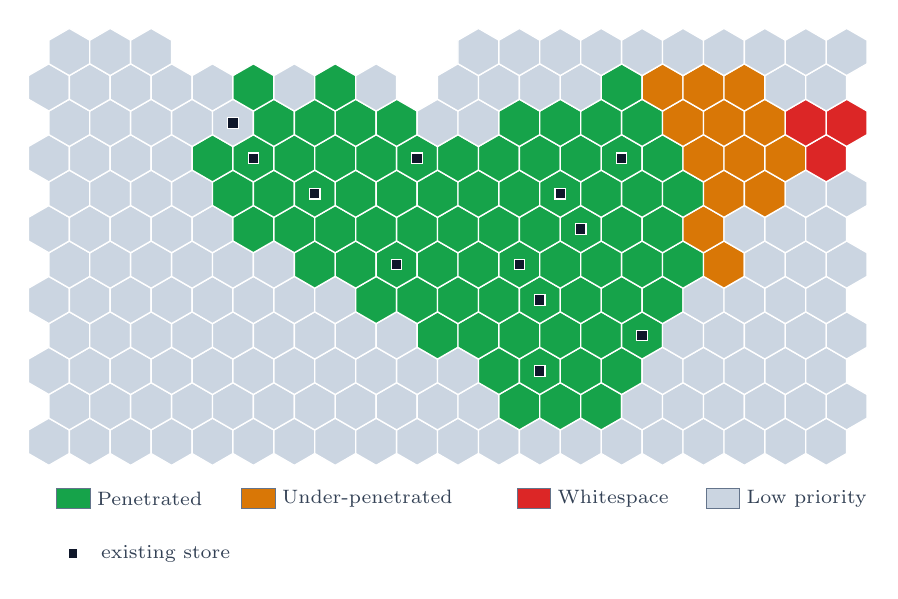
\begin{tikzpicture}
\fill[clsLow, draw=white, line width=0.5pt] (0.260,0.150) -- (0.000,0.300) -- (-0.260,0.150) -- (-0.260,-0.150) -- (-0.000,-0.300) -- (0.260,-0.150) -- cycle;
\fill[clsLow, draw=white, line width=0.5pt] (0.779,0.150) -- (0.520,0.300) -- (0.260,0.150) -- (0.260,-0.150) -- (0.520,-0.300) -- (0.779,-0.150) -- cycle;
\fill[clsLow, draw=white, line width=0.5pt] (1.299,0.150) -- (1.039,0.300) -- (0.779,0.150) -- (0.779,-0.150) -- (1.039,-0.300) -- (1.299,-0.150) -- cycle;
\fill[clsLow, draw=white, line width=0.5pt] (1.819,0.150) -- (1.559,0.300) -- (1.299,0.150) -- (1.299,-0.150) -- (1.559,-0.300) -- (1.819,-0.150) -- cycle;
\fill[clsLow, draw=white, line width=0.5pt] (2.338,0.150) -- (2.078,0.300) -- (1.819,0.150) -- (1.819,-0.150) -- (2.078,-0.300) -- (2.338,-0.150) -- cycle;
\fill[clsLow, draw=white, line width=0.5pt] (2.858,0.150) -- (2.598,0.300) -- (2.338,0.150) -- (2.338,-0.150) -- (2.598,-0.300) -- (2.858,-0.150) -- cycle;
\fill[clsLow, draw=white, line width=0.5pt] (3.377,0.150) -- (3.118,0.300) -- (2.858,0.150) -- (2.858,-0.150) -- (3.118,-0.300) -- (3.377,-0.150) -- cycle;
\fill[clsLow, draw=white, line width=0.5pt] (3.897,0.150) -- (3.637,0.300) -- (3.377,0.150) -- (3.377,-0.150) -- (3.637,-0.300) -- (3.897,-0.150) -- cycle;
\fill[clsLow, draw=white, line width=0.5pt] (4.417,0.150) -- (4.157,0.300) -- (3.897,0.150) -- (3.897,-0.150) -- (4.157,-0.300) -- (4.417,-0.150) -- cycle;
\fill[clsLow, draw=white, line width=0.5pt] (4.936,0.150) -- (4.677,0.300) -- (4.417,0.150) -- (4.417,-0.150) -- (4.677,-0.300) -- (4.936,-0.150) -- cycle;
\fill[clsLow, draw=white, line width=0.5pt] (5.456,0.150) -- (5.196,0.300) -- (4.936,0.150) -- (4.936,-0.150) -- (5.196,-0.300) -- (5.456,-0.150) -- cycle;
\fill[clsLow, draw=white, line width=0.5pt] (5.976,0.150) -- (5.716,0.300) -- (5.456,0.150) -- (5.456,-0.150) -- (5.716,-0.300) -- (5.976,-0.150) -- cycle;
\fill[clsLow, draw=white, line width=0.5pt] (6.495,0.150) -- (6.235,0.300) -- (5.976,0.150) -- (5.976,-0.150) -- (6.235,-0.300) -- (6.495,-0.150) -- cycle;
\fill[clsLow, draw=white, line width=0.5pt] (7.015,0.150) -- (6.755,0.300) -- (6.495,0.150) -- (6.495,-0.150) -- (6.755,-0.300) -- (7.015,-0.150) -- cycle;
\fill[clsLow, draw=white, line width=0.5pt] (7.534,0.150) -- (7.275,0.300) -- (7.015,0.150) -- (7.015,-0.150) -- (7.275,-0.300) -- (7.534,-0.150) -- cycle;
\fill[clsLow, draw=white, line width=0.5pt] (8.054,0.150) -- (7.794,0.300) -- (7.534,0.150) -- (7.534,-0.150) -- (7.794,-0.300) -- (8.054,-0.150) -- cycle;
\fill[clsLow, draw=white, line width=0.5pt] (8.574,0.150) -- (8.314,0.300) -- (8.054,0.150) -- (8.054,-0.150) -- (8.314,-0.300) -- (8.574,-0.150) -- cycle;
\fill[clsLow, draw=white, line width=0.5pt] (9.093,0.150) -- (8.833,0.300) -- (8.574,0.150) -- (8.574,-0.150) -- (8.833,-0.300) -- (9.093,-0.150) -- cycle;
\fill[clsLow, draw=white, line width=0.5pt] (9.613,0.150) -- (9.353,0.300) -- (9.093,0.150) -- (9.093,-0.150) -- (9.353,-0.300) -- (9.613,-0.150) -- cycle;
\fill[clsLow, draw=white, line width=0.5pt] (10.132,0.150) -- (9.873,0.300) -- (9.613,0.150) -- (9.613,-0.150) -- (9.873,-0.300) -- (10.132,-0.150) -- cycle;
\fill[clsLow, draw=white, line width=0.5pt] (0.520,0.600) -- (0.260,0.750) -- (-0.000,0.600) -- (0.000,0.300) -- (0.260,0.150) -- (0.520,0.300) -- cycle;
\fill[clsLow, draw=white, line width=0.5pt] (1.039,0.600) -- (0.779,0.750) -- (0.520,0.600) -- (0.520,0.300) -- (0.779,0.150) -- (1.039,0.300) -- cycle;
\fill[clsLow, draw=white, line width=0.5pt] (1.559,0.600) -- (1.299,0.750) -- (1.039,0.600) -- (1.039,0.300) -- (1.299,0.150) -- (1.559,0.300) -- cycle;
\fill[clsLow, draw=white, line width=0.5pt] (2.078,0.600) -- (1.819,0.750) -- (1.559,0.600) -- (1.559,0.300) -- (1.819,0.150) -- (2.078,0.300) -- cycle;
\fill[clsLow, draw=white, line width=0.5pt] (2.598,0.600) -- (2.338,0.750) -- (2.078,0.600) -- (2.078,0.300) -- (2.338,0.150) -- (2.598,0.300) -- cycle;
\fill[clsLow, draw=white, line width=0.5pt] (3.118,0.600) -- (2.858,0.750) -- (2.598,0.600) -- (2.598,0.300) -- (2.858,0.150) -- (3.118,0.300) -- cycle;
\fill[clsLow, draw=white, line width=0.5pt] (3.637,0.600) -- (3.377,0.750) -- (3.118,0.600) -- (3.118,0.300) -- (3.377,0.150) -- (3.637,0.300) -- cycle;
\fill[clsLow, draw=white, line width=0.5pt] (4.157,0.600) -- (3.897,0.750) -- (3.637,0.600) -- (3.637,0.300) -- (3.897,0.150) -- (4.157,0.300) -- cycle;
\fill[clsLow, draw=white, line width=0.5pt] (4.677,0.600) -- (4.417,0.750) -- (4.157,0.600) -- (4.157,0.300) -- (4.417,0.150) -- (4.677,0.300) -- cycle;
\fill[clsLow, draw=white, line width=0.5pt] (5.196,0.600) -- (4.936,0.750) -- (4.677,0.600) -- (4.677,0.300) -- (4.936,0.150) -- (5.196,0.300) -- cycle;
\fill[clsLow, draw=white, line width=0.5pt] (5.716,0.600) -- (5.456,0.750) -- (5.196,0.600) -- (5.196,0.300) -- (5.456,0.150) -- (5.716,0.300) -- cycle;
\fill[clsPen, draw=white, line width=0.5pt] (6.235,0.600) -- (5.976,0.750) -- (5.716,0.600) -- (5.716,0.300) -- (5.976,0.150) -- (6.235,0.300) -- cycle;
\fill[clsPen, draw=white, line width=0.5pt] (6.755,0.600) -- (6.495,0.750) -- (6.235,0.600) -- (6.235,0.300) -- (6.495,0.150) -- (6.755,0.300) -- cycle;
\fill[clsPen, draw=white, line width=0.5pt] (7.275,0.600) -- (7.015,0.750) -- (6.755,0.600) -- (6.755,0.300) -- (7.015,0.150) -- (7.275,0.300) -- cycle;
\fill[clsLow, draw=white, line width=0.5pt] (7.794,0.600) -- (7.534,0.750) -- (7.275,0.600) -- (7.275,0.300) -- (7.534,0.150) -- (7.794,0.300) -- cycle;
\fill[clsLow, draw=white, line width=0.5pt] (8.314,0.600) -- (8.054,0.750) -- (7.794,0.600) -- (7.794,0.300) -- (8.054,0.150) -- (8.314,0.300) -- cycle;
\fill[clsLow, draw=white, line width=0.5pt] (8.833,0.600) -- (8.574,0.750) -- (8.314,0.600) -- (8.314,0.300) -- (8.574,0.150) -- (8.833,0.300) -- cycle;
\fill[clsLow, draw=white, line width=0.5pt] (9.353,0.600) -- (9.093,0.750) -- (8.833,0.600) -- (8.833,0.300) -- (9.093,0.150) -- (9.353,0.300) -- cycle;
\fill[clsLow, draw=white, line width=0.5pt] (9.873,0.600) -- (9.613,0.750) -- (9.353,0.600) -- (9.353,0.300) -- (9.613,0.150) -- (9.873,0.300) -- cycle;
\fill[clsLow, draw=white, line width=0.5pt] (10.392,0.600) -- (10.132,0.750) -- (9.873,0.600) -- (9.873,0.300) -- (10.132,0.150) -- (10.392,0.300) -- cycle;
\fill[clsLow, draw=white, line width=0.5pt] (0.260,1.050) -- (0.000,1.200) -- (-0.260,1.050) -- (-0.260,0.750) -- (-0.000,0.600) -- (0.260,0.750) -- cycle;
\fill[clsLow, draw=white, line width=0.5pt] (0.779,1.050) -- (0.520,1.200) -- (0.260,1.050) -- (0.260,0.750) -- (0.520,0.600) -- (0.779,0.750) -- cycle;
\fill[clsLow, draw=white, line width=0.5pt] (1.299,1.050) -- (1.039,1.200) -- (0.779,1.050) -- (0.779,0.750) -- (1.039,0.600) -- (1.299,0.750) -- cycle;
\fill[clsLow, draw=white, line width=0.5pt] (1.819,1.050) -- (1.559,1.200) -- (1.299,1.050) -- (1.299,0.750) -- (1.559,0.600) -- (1.819,0.750) -- cycle;
\fill[clsLow, draw=white, line width=0.5pt] (2.338,1.050) -- (2.078,1.200) -- (1.819,1.050) -- (1.819,0.750) -- (2.078,0.600) -- (2.338,0.750) -- cycle;
\fill[clsLow, draw=white, line width=0.5pt] (2.858,1.050) -- (2.598,1.200) -- (2.338,1.050) -- (2.338,0.750) -- (2.598,0.600) -- (2.858,0.750) -- cycle;
\fill[clsLow, draw=white, line width=0.5pt] (3.377,1.050) -- (3.118,1.200) -- (2.858,1.050) -- (2.858,0.750) -- (3.118,0.600) -- (3.377,0.750) -- cycle;
\fill[clsLow, draw=white, line width=0.5pt] (3.897,1.050) -- (3.637,1.200) -- (3.377,1.050) -- (3.377,0.750) -- (3.637,0.600) -- (3.897,0.750) -- cycle;
\fill[clsLow, draw=white, line width=0.5pt] (4.417,1.050) -- (4.157,1.200) -- (3.897,1.050) -- (3.897,0.750) -- (4.157,0.600) -- (4.417,0.750) -- cycle;
\fill[clsLow, draw=white, line width=0.5pt] (4.936,1.050) -- (4.677,1.200) -- (4.417,1.050) -- (4.417,0.750) -- (4.677,0.600) -- (4.936,0.750) -- cycle;
\fill[clsLow, draw=white, line width=0.5pt] (5.456,1.050) -- (5.196,1.200) -- (4.936,1.050) -- (4.936,0.750) -- (5.196,0.600) -- (5.456,0.750) -- cycle;
\fill[clsPen, draw=white, line width=0.5pt] (5.976,1.050) -- (5.716,1.200) -- (5.456,1.050) -- (5.456,0.750) -- (5.716,0.600) -- (5.976,0.750) -- cycle;
\fill[clsPen, draw=white, line width=0.5pt] (6.495,1.050) -- (6.235,1.200) -- (5.976,1.050) -- (5.976,0.750) -- (6.235,0.600) -- (6.495,0.750) -- cycle;
\fill[clsPen, draw=white, line width=0.5pt] (7.015,1.050) -- (6.755,1.200) -- (6.495,1.050) -- (6.495,0.750) -- (6.755,0.600) -- (7.015,0.750) -- cycle;
\fill[clsPen, draw=white, line width=0.5pt] (7.534,1.050) -- (7.275,1.200) -- (7.015,1.050) -- (7.015,0.750) -- (7.275,0.600) -- (7.534,0.750) -- cycle;
\fill[clsLow, draw=white, line width=0.5pt] (8.054,1.050) -- (7.794,1.200) -- (7.534,1.050) -- (7.534,0.750) -- (7.794,0.600) -- (8.054,0.750) -- cycle;
\fill[clsLow, draw=white, line width=0.5pt] (8.574,1.050) -- (8.314,1.200) -- (8.054,1.050) -- (8.054,0.750) -- (8.314,0.600) -- (8.574,0.750) -- cycle;
\fill[clsLow, draw=white, line width=0.5pt] (9.093,1.050) -- (8.833,1.200) -- (8.574,1.050) -- (8.574,0.750) -- (8.833,0.600) -- (9.093,0.750) -- cycle;
\fill[clsLow, draw=white, line width=0.5pt] (9.613,1.050) -- (9.353,1.200) -- (9.093,1.050) -- (9.093,0.750) -- (9.353,0.600) -- (9.613,0.750) -- cycle;
\fill[clsLow, draw=white, line width=0.5pt] (10.132,1.050) -- (9.873,1.200) -- (9.613,1.050) -- (9.613,0.750) -- (9.873,0.600) -- (10.132,0.750) -- cycle;
\fill[clsLow, draw=white, line width=0.5pt] (0.520,1.500) -- (0.260,1.650) -- (-0.000,1.500) -- (0.000,1.200) -- (0.260,1.050) -- (0.520,1.200) -- cycle;
\fill[clsLow, draw=white, line width=0.5pt] (1.039,1.500) -- (0.779,1.650) -- (0.520,1.500) -- (0.520,1.200) -- (0.779,1.050) -- (1.039,1.200) -- cycle;
\fill[clsLow, draw=white, line width=0.5pt] (1.559,1.500) -- (1.299,1.650) -- (1.039,1.500) -- (1.039,1.200) -- (1.299,1.050) -- (1.559,1.200) -- cycle;
\fill[clsLow, draw=white, line width=0.5pt] (2.078,1.500) -- (1.819,1.650) -- (1.559,1.500) -- (1.559,1.200) -- (1.819,1.050) -- (2.078,1.200) -- cycle;
\fill[clsLow, draw=white, line width=0.5pt] (2.598,1.500) -- (2.338,1.650) -- (2.078,1.500) -- (2.078,1.200) -- (2.338,1.050) -- (2.598,1.200) -- cycle;
\fill[clsLow, draw=white, line width=0.5pt] (3.118,1.500) -- (2.858,1.650) -- (2.598,1.500) -- (2.598,1.200) -- (2.858,1.050) -- (3.118,1.200) -- cycle;
\fill[clsLow, draw=white, line width=0.5pt] (3.637,1.500) -- (3.377,1.650) -- (3.118,1.500) -- (3.118,1.200) -- (3.377,1.050) -- (3.637,1.200) -- cycle;
\fill[clsLow, draw=white, line width=0.5pt] (4.157,1.500) -- (3.897,1.650) -- (3.637,1.500) -- (3.637,1.200) -- (3.897,1.050) -- (4.157,1.200) -- cycle;
\fill[clsLow, draw=white, line width=0.5pt] (4.677,1.500) -- (4.417,1.650) -- (4.157,1.500) -- (4.157,1.200) -- (4.417,1.050) -- (4.677,1.200) -- cycle;
\fill[clsPen, draw=white, line width=0.5pt] (5.196,1.500) -- (4.936,1.650) -- (4.677,1.500) -- (4.677,1.200) -- (4.936,1.050) -- (5.196,1.200) -- cycle;
\fill[clsPen, draw=white, line width=0.5pt] (5.716,1.500) -- (5.456,1.650) -- (5.196,1.500) -- (5.196,1.200) -- (5.456,1.050) -- (5.716,1.200) -- cycle;
\fill[clsPen, draw=white, line width=0.5pt] (6.235,1.500) -- (5.976,1.650) -- (5.716,1.500) -- (5.716,1.200) -- (5.976,1.050) -- (6.235,1.200) -- cycle;
\fill[clsPen, draw=white, line width=0.5pt] (6.755,1.500) -- (6.495,1.650) -- (6.235,1.500) -- (6.235,1.200) -- (6.495,1.050) -- (6.755,1.200) -- cycle;
\fill[clsPen, draw=white, line width=0.5pt] (7.275,1.500) -- (7.015,1.650) -- (6.755,1.500) -- (6.755,1.200) -- (7.015,1.050) -- (7.275,1.200) -- cycle;
\fill[clsPen, draw=white, line width=0.5pt] (7.794,1.500) -- (7.534,1.650) -- (7.275,1.500) -- (7.275,1.200) -- (7.534,1.050) -- (7.794,1.200) -- cycle;
\fill[clsLow, draw=white, line width=0.5pt] (8.314,1.500) -- (8.054,1.650) -- (7.794,1.500) -- (7.794,1.200) -- (8.054,1.050) -- (8.314,1.200) -- cycle;
\fill[clsLow, draw=white, line width=0.5pt] (8.833,1.500) -- (8.574,1.650) -- (8.314,1.500) -- (8.314,1.200) -- (8.574,1.050) -- (8.833,1.200) -- cycle;
\fill[clsLow, draw=white, line width=0.5pt] (9.353,1.500) -- (9.093,1.650) -- (8.833,1.500) -- (8.833,1.200) -- (9.093,1.050) -- (9.353,1.200) -- cycle;
\fill[clsLow, draw=white, line width=0.5pt] (9.873,1.500) -- (9.613,1.650) -- (9.353,1.500) -- (9.353,1.200) -- (9.613,1.050) -- (9.873,1.200) -- cycle;
\fill[clsLow, draw=white, line width=0.5pt] (10.392,1.500) -- (10.132,1.650) -- (9.873,1.500) -- (9.873,1.200) -- (10.132,1.050) -- (10.392,1.200) -- cycle;
\fill[clsLow, draw=white, line width=0.5pt] (0.260,1.950) -- (0.000,2.100) -- (-0.260,1.950) -- (-0.260,1.650) -- (-0.000,1.500) -- (0.260,1.650) -- cycle;
\fill[clsLow, draw=white, line width=0.5pt] (0.779,1.950) -- (0.520,2.100) -- (0.260,1.950) -- (0.260,1.650) -- (0.520,1.500) -- (0.779,1.650) -- cycle;
\fill[clsLow, draw=white, line width=0.5pt] (1.299,1.950) -- (1.039,2.100) -- (0.779,1.950) -- (0.779,1.650) -- (1.039,1.500) -- (1.299,1.650) -- cycle;
\fill[clsLow, draw=white, line width=0.5pt] (1.819,1.950) -- (1.559,2.100) -- (1.299,1.950) -- (1.299,1.650) -- (1.559,1.500) -- (1.819,1.650) -- cycle;
\fill[clsLow, draw=white, line width=0.5pt] (2.338,1.950) -- (2.078,2.100) -- (1.819,1.950) -- (1.819,1.650) -- (2.078,1.500) -- (2.338,1.650) -- cycle;
\fill[clsLow, draw=white, line width=0.5pt] (2.858,1.950) -- (2.598,2.100) -- (2.338,1.950) -- (2.338,1.650) -- (2.598,1.500) -- (2.858,1.650) -- cycle;
\fill[clsLow, draw=white, line width=0.5pt] (3.377,1.950) -- (3.118,2.100) -- (2.858,1.950) -- (2.858,1.650) -- (3.118,1.500) -- (3.377,1.650) -- cycle;
\fill[clsLow, draw=white, line width=0.5pt] (3.897,1.950) -- (3.637,2.100) -- (3.377,1.950) -- (3.377,1.650) -- (3.637,1.500) -- (3.897,1.650) -- cycle;
\fill[clsPen, draw=white, line width=0.5pt] (4.417,1.950) -- (4.157,2.100) -- (3.897,1.950) -- (3.897,1.650) -- (4.157,1.500) -- (4.417,1.650) -- cycle;
\fill[clsPen, draw=white, line width=0.5pt] (4.936,1.950) -- (4.677,2.100) -- (4.417,1.950) -- (4.417,1.650) -- (4.677,1.500) -- (4.936,1.650) -- cycle;
\fill[clsPen, draw=white, line width=0.5pt] (5.456,1.950) -- (5.196,2.100) -- (4.936,1.950) -- (4.936,1.650) -- (5.196,1.500) -- (5.456,1.650) -- cycle;
\fill[clsPen, draw=white, line width=0.5pt] (5.976,1.950) -- (5.716,2.100) -- (5.456,1.950) -- (5.456,1.650) -- (5.716,1.500) -- (5.976,1.650) -- cycle;
\fill[clsPen, draw=white, line width=0.5pt] (6.495,1.950) -- (6.235,2.100) -- (5.976,1.950) -- (5.976,1.650) -- (6.235,1.500) -- (6.495,1.650) -- cycle;
\fill[clsPen, draw=white, line width=0.5pt] (7.015,1.950) -- (6.755,2.100) -- (6.495,1.950) -- (6.495,1.650) -- (6.755,1.500) -- (7.015,1.650) -- cycle;
\fill[clsPen, draw=white, line width=0.5pt] (7.534,1.950) -- (7.275,2.100) -- (7.015,1.950) -- (7.015,1.650) -- (7.275,1.500) -- (7.534,1.650) -- cycle;
\fill[clsPen, draw=white, line width=0.5pt] (8.054,1.950) -- (7.794,2.100) -- (7.534,1.950) -- (7.534,1.650) -- (7.794,1.500) -- (8.054,1.650) -- cycle;
\fill[clsLow, draw=white, line width=0.5pt] (8.574,1.950) -- (8.314,2.100) -- (8.054,1.950) -- (8.054,1.650) -- (8.314,1.500) -- (8.574,1.650) -- cycle;
\fill[clsLow, draw=white, line width=0.5pt] (9.093,1.950) -- (8.833,2.100) -- (8.574,1.950) -- (8.574,1.650) -- (8.833,1.500) -- (9.093,1.650) -- cycle;
\fill[clsLow, draw=white, line width=0.5pt] (9.613,1.950) -- (9.353,2.100) -- (9.093,1.950) -- (9.093,1.650) -- (9.353,1.500) -- (9.613,1.650) -- cycle;
\fill[clsLow, draw=white, line width=0.5pt] (10.132,1.950) -- (9.873,2.100) -- (9.613,1.950) -- (9.613,1.650) -- (9.873,1.500) -- (10.132,1.650) -- cycle;
\fill[clsLow, draw=white, line width=0.5pt] (0.520,2.400) -- (0.260,2.550) -- (-0.000,2.400) -- (0.000,2.100) -- (0.260,1.950) -- (0.520,2.100) -- cycle;
\fill[clsLow, draw=white, line width=0.5pt] (1.039,2.400) -- (0.779,2.550) -- (0.520,2.400) -- (0.520,2.100) -- (0.779,1.950) -- (1.039,2.100) -- cycle;
\fill[clsLow, draw=white, line width=0.5pt] (1.559,2.400) -- (1.299,2.550) -- (1.039,2.400) -- (1.039,2.100) -- (1.299,1.950) -- (1.559,2.100) -- cycle;
\fill[clsLow, draw=white, line width=0.5pt] (2.078,2.400) -- (1.819,2.550) -- (1.559,2.400) -- (1.559,2.100) -- (1.819,1.950) -- (2.078,2.100) -- cycle;
\fill[clsLow, draw=white, line width=0.5pt] (2.598,2.400) -- (2.338,2.550) -- (2.078,2.400) -- (2.078,2.100) -- (2.338,1.950) -- (2.598,2.100) -- cycle;
\fill[clsLow, draw=white, line width=0.5pt] (3.118,2.400) -- (2.858,2.550) -- (2.598,2.400) -- (2.598,2.100) -- (2.858,1.950) -- (3.118,2.100) -- cycle;
\fill[clsPen, draw=white, line width=0.5pt] (3.637,2.400) -- (3.377,2.550) -- (3.118,2.400) -- (3.118,2.100) -- (3.377,1.950) -- (3.637,2.100) -- cycle;
\fill[clsPen, draw=white, line width=0.5pt] (4.157,2.400) -- (3.897,2.550) -- (3.637,2.400) -- (3.637,2.100) -- (3.897,1.950) -- (4.157,2.100) -- cycle;
\fill[clsPen, draw=white, line width=0.5pt] (4.677,2.400) -- (4.417,2.550) -- (4.157,2.400) -- (4.157,2.100) -- (4.417,1.950) -- (4.677,2.100) -- cycle;
\fill[clsPen, draw=white, line width=0.5pt] (5.196,2.400) -- (4.936,2.550) -- (4.677,2.400) -- (4.677,2.100) -- (4.936,1.950) -- (5.196,2.100) -- cycle;
\fill[clsPen, draw=white, line width=0.5pt] (5.716,2.400) -- (5.456,2.550) -- (5.196,2.400) -- (5.196,2.100) -- (5.456,1.950) -- (5.716,2.100) -- cycle;
\fill[clsPen, draw=white, line width=0.5pt] (6.235,2.400) -- (5.976,2.550) -- (5.716,2.400) -- (5.716,2.100) -- (5.976,1.950) -- (6.235,2.100) -- cycle;
\fill[clsPen, draw=white, line width=0.5pt] (6.755,2.400) -- (6.495,2.550) -- (6.235,2.400) -- (6.235,2.100) -- (6.495,1.950) -- (6.755,2.100) -- cycle;
\fill[clsPen, draw=white, line width=0.5pt] (7.275,2.400) -- (7.015,2.550) -- (6.755,2.400) -- (6.755,2.100) -- (7.015,1.950) -- (7.275,2.100) -- cycle;
\fill[clsPen, draw=white, line width=0.5pt] (7.794,2.400) -- (7.534,2.550) -- (7.275,2.400) -- (7.275,2.100) -- (7.534,1.950) -- (7.794,2.100) -- cycle;
\fill[clsPen, draw=white, line width=0.5pt] (8.314,2.400) -- (8.054,2.550) -- (7.794,2.400) -- (7.794,2.100) -- (8.054,1.950) -- (8.314,2.100) -- cycle;
\fill[clsUnd, draw=white, line width=0.5pt] (8.833,2.400) -- (8.574,2.550) -- (8.314,2.400) -- (8.314,2.100) -- (8.574,1.950) -- (8.833,2.100) -- cycle;
\fill[clsLow, draw=white, line width=0.5pt] (9.353,2.400) -- (9.093,2.550) -- (8.833,2.400) -- (8.833,2.100) -- (9.093,1.950) -- (9.353,2.100) -- cycle;
\fill[clsLow, draw=white, line width=0.5pt] (9.873,2.400) -- (9.613,2.550) -- (9.353,2.400) -- (9.353,2.100) -- (9.613,1.950) -- (9.873,2.100) -- cycle;
\fill[clsLow, draw=white, line width=0.5pt] (10.392,2.400) -- (10.132,2.550) -- (9.873,2.400) -- (9.873,2.100) -- (10.132,1.950) -- (10.392,2.100) -- cycle;
\fill[clsLow, draw=white, line width=0.5pt] (0.260,2.850) -- (0.000,3.000) -- (-0.260,2.850) -- (-0.260,2.550) -- (-0.000,2.400) -- (0.260,2.550) -- cycle;
\fill[clsLow, draw=white, line width=0.5pt] (0.779,2.850) -- (0.520,3.000) -- (0.260,2.850) -- (0.260,2.550) -- (0.520,2.400) -- (0.779,2.550) -- cycle;
\fill[clsLow, draw=white, line width=0.5pt] (1.299,2.850) -- (1.039,3.000) -- (0.779,2.850) -- (0.779,2.550) -- (1.039,2.400) -- (1.299,2.550) -- cycle;
\fill[clsLow, draw=white, line width=0.5pt] (1.819,2.850) -- (1.559,3.000) -- (1.299,2.850) -- (1.299,2.550) -- (1.559,2.400) -- (1.819,2.550) -- cycle;
\fill[clsLow, draw=white, line width=0.5pt] (2.338,2.850) -- (2.078,3.000) -- (1.819,2.850) -- (1.819,2.550) -- (2.078,2.400) -- (2.338,2.550) -- cycle;
\fill[clsPen, draw=white, line width=0.5pt] (2.858,2.850) -- (2.598,3.000) -- (2.338,2.850) -- (2.338,2.550) -- (2.598,2.400) -- (2.858,2.550) -- cycle;
\fill[clsPen, draw=white, line width=0.5pt] (3.377,2.850) -- (3.118,3.000) -- (2.858,2.850) -- (2.858,2.550) -- (3.118,2.400) -- (3.377,2.550) -- cycle;
\fill[clsPen, draw=white, line width=0.5pt] (3.897,2.850) -- (3.637,3.000) -- (3.377,2.850) -- (3.377,2.550) -- (3.637,2.400) -- (3.897,2.550) -- cycle;
\fill[clsPen, draw=white, line width=0.5pt] (4.417,2.850) -- (4.157,3.000) -- (3.897,2.850) -- (3.897,2.550) -- (4.157,2.400) -- (4.417,2.550) -- cycle;
\fill[clsPen, draw=white, line width=0.5pt] (4.936,2.850) -- (4.677,3.000) -- (4.417,2.850) -- (4.417,2.550) -- (4.677,2.400) -- (4.936,2.550) -- cycle;
\fill[clsPen, draw=white, line width=0.5pt] (5.456,2.850) -- (5.196,3.000) -- (4.936,2.850) -- (4.936,2.550) -- (5.196,2.400) -- (5.456,2.550) -- cycle;
\fill[clsPen, draw=white, line width=0.5pt] (5.976,2.850) -- (5.716,3.000) -- (5.456,2.850) -- (5.456,2.550) -- (5.716,2.400) -- (5.976,2.550) -- cycle;
\fill[clsPen, draw=white, line width=0.5pt] (6.495,2.850) -- (6.235,3.000) -- (5.976,2.850) -- (5.976,2.550) -- (6.235,2.400) -- (6.495,2.550) -- cycle;
\fill[clsPen, draw=white, line width=0.5pt] (7.015,2.850) -- (6.755,3.000) -- (6.495,2.850) -- (6.495,2.550) -- (6.755,2.400) -- (7.015,2.550) -- cycle;
\fill[clsPen, draw=white, line width=0.5pt] (7.534,2.850) -- (7.275,3.000) -- (7.015,2.850) -- (7.015,2.550) -- (7.275,2.400) -- (7.534,2.550) -- cycle;
\fill[clsPen, draw=white, line width=0.5pt] (8.054,2.850) -- (7.794,3.000) -- (7.534,2.850) -- (7.534,2.550) -- (7.794,2.400) -- (8.054,2.550) -- cycle;
\fill[clsUnd, draw=white, line width=0.5pt] (8.574,2.850) -- (8.314,3.000) -- (8.054,2.850) -- (8.054,2.550) -- (8.314,2.400) -- (8.574,2.550) -- cycle;
\fill[clsLow, draw=white, line width=0.5pt] (9.093,2.850) -- (8.833,3.000) -- (8.574,2.850) -- (8.574,2.550) -- (8.833,2.400) -- (9.093,2.550) -- cycle;
\fill[clsLow, draw=white, line width=0.5pt] (9.613,2.850) -- (9.353,3.000) -- (9.093,2.850) -- (9.093,2.550) -- (9.353,2.400) -- (9.613,2.550) -- cycle;
\fill[clsLow, draw=white, line width=0.5pt] (10.132,2.850) -- (9.873,3.000) -- (9.613,2.850) -- (9.613,2.550) -- (9.873,2.400) -- (10.132,2.550) -- cycle;
\fill[clsLow, draw=white, line width=0.5pt] (0.520,3.300) -- (0.260,3.450) -- (-0.000,3.300) -- (0.000,3.000) -- (0.260,2.850) -- (0.520,3.000) -- cycle;
\fill[clsLow, draw=white, line width=0.5pt] (1.039,3.300) -- (0.779,3.450) -- (0.520,3.300) -- (0.520,3.000) -- (0.779,2.850) -- (1.039,3.000) -- cycle;
\fill[clsLow, draw=white, line width=0.5pt] (1.559,3.300) -- (1.299,3.450) -- (1.039,3.300) -- (1.039,3.000) -- (1.299,2.850) -- (1.559,3.000) -- cycle;
\fill[clsLow, draw=white, line width=0.5pt] (2.078,3.300) -- (1.819,3.450) -- (1.559,3.300) -- (1.559,3.000) -- (1.819,2.850) -- (2.078,3.000) -- cycle;
\fill[clsPen, draw=white, line width=0.5pt] (2.598,3.300) -- (2.338,3.450) -- (2.078,3.300) -- (2.078,3.000) -- (2.338,2.850) -- (2.598,3.000) -- cycle;
\fill[clsPen, draw=white, line width=0.5pt] (3.118,3.300) -- (2.858,3.450) -- (2.598,3.300) -- (2.598,3.000) -- (2.858,2.850) -- (3.118,3.000) -- cycle;
\fill[clsPen, draw=white, line width=0.5pt] (3.637,3.300) -- (3.377,3.450) -- (3.118,3.300) -- (3.118,3.000) -- (3.377,2.850) -- (3.637,3.000) -- cycle;
\fill[clsPen, draw=white, line width=0.5pt] (4.157,3.300) -- (3.897,3.450) -- (3.637,3.300) -- (3.637,3.000) -- (3.897,2.850) -- (4.157,3.000) -- cycle;
\fill[clsPen, draw=white, line width=0.5pt] (4.677,3.300) -- (4.417,3.450) -- (4.157,3.300) -- (4.157,3.000) -- (4.417,2.850) -- (4.677,3.000) -- cycle;
\fill[clsPen, draw=white, line width=0.5pt] (5.196,3.300) -- (4.936,3.450) -- (4.677,3.300) -- (4.677,3.000) -- (4.936,2.850) -- (5.196,3.000) -- cycle;
\fill[clsPen, draw=white, line width=0.5pt] (5.716,3.300) -- (5.456,3.450) -- (5.196,3.300) -- (5.196,3.000) -- (5.456,2.850) -- (5.716,3.000) -- cycle;
\fill[clsPen, draw=white, line width=0.5pt] (6.235,3.300) -- (5.976,3.450) -- (5.716,3.300) -- (5.716,3.000) -- (5.976,2.850) -- (6.235,3.000) -- cycle;
\fill[clsPen, draw=white, line width=0.5pt] (6.755,3.300) -- (6.495,3.450) -- (6.235,3.300) -- (6.235,3.000) -- (6.495,2.850) -- (6.755,3.000) -- cycle;
\fill[clsPen, draw=white, line width=0.5pt] (7.275,3.300) -- (7.015,3.450) -- (6.755,3.300) -- (6.755,3.000) -- (7.015,2.850) -- (7.275,3.000) -- cycle;
\fill[clsPen, draw=white, line width=0.5pt] (7.794,3.300) -- (7.534,3.450) -- (7.275,3.300) -- (7.275,3.000) -- (7.534,2.850) -- (7.794,3.000) -- cycle;
\fill[clsPen, draw=white, line width=0.5pt] (8.314,3.300) -- (8.054,3.450) -- (7.794,3.300) -- (7.794,3.000) -- (8.054,2.850) -- (8.314,3.000) -- cycle;
\fill[clsUnd, draw=white, line width=0.5pt] (8.833,3.300) -- (8.574,3.450) -- (8.314,3.300) -- (8.314,3.000) -- (8.574,2.850) -- (8.833,3.000) -- cycle;
\fill[clsUnd, draw=white, line width=0.5pt] (9.353,3.300) -- (9.093,3.450) -- (8.833,3.300) -- (8.833,3.000) -- (9.093,2.850) -- (9.353,3.000) -- cycle;
\fill[clsLow, draw=white, line width=0.5pt] (9.873,3.300) -- (9.613,3.450) -- (9.353,3.300) -- (9.353,3.000) -- (9.613,2.850) -- (9.873,3.000) -- cycle;
\fill[clsLow, draw=white, line width=0.5pt] (10.392,3.300) -- (10.132,3.450) -- (9.873,3.300) -- (9.873,3.000) -- (10.132,2.850) -- (10.392,3.000) -- cycle;
\fill[clsLow, draw=white, line width=0.5pt] (0.260,3.750) -- (0.000,3.900) -- (-0.260,3.750) -- (-0.260,3.450) -- (-0.000,3.300) -- (0.260,3.450) -- cycle;
\fill[clsLow, draw=white, line width=0.5pt] (0.779,3.750) -- (0.520,3.900) -- (0.260,3.750) -- (0.260,3.450) -- (0.520,3.300) -- (0.779,3.450) -- cycle;
\fill[clsLow, draw=white, line width=0.5pt] (1.299,3.750) -- (1.039,3.900) -- (0.779,3.750) -- (0.779,3.450) -- (1.039,3.300) -- (1.299,3.450) -- cycle;
\fill[clsLow, draw=white, line width=0.5pt] (1.819,3.750) -- (1.559,3.900) -- (1.299,3.750) -- (1.299,3.450) -- (1.559,3.300) -- (1.819,3.450) -- cycle;
\fill[clsPen, draw=white, line width=0.5pt] (2.338,3.750) -- (2.078,3.900) -- (1.819,3.750) -- (1.819,3.450) -- (2.078,3.300) -- (2.338,3.450) -- cycle;
\fill[clsPen, draw=white, line width=0.5pt] (2.858,3.750) -- (2.598,3.900) -- (2.338,3.750) -- (2.338,3.450) -- (2.598,3.300) -- (2.858,3.450) -- cycle;
\fill[clsPen, draw=white, line width=0.5pt] (3.377,3.750) -- (3.118,3.900) -- (2.858,3.750) -- (2.858,3.450) -- (3.118,3.300) -- (3.377,3.450) -- cycle;
\fill[clsPen, draw=white, line width=0.5pt] (3.897,3.750) -- (3.637,3.900) -- (3.377,3.750) -- (3.377,3.450) -- (3.637,3.300) -- (3.897,3.450) -- cycle;
\fill[clsPen, draw=white, line width=0.5pt] (4.417,3.750) -- (4.157,3.900) -- (3.897,3.750) -- (3.897,3.450) -- (4.157,3.300) -- (4.417,3.450) -- cycle;
\fill[clsPen, draw=white, line width=0.5pt] (4.936,3.750) -- (4.677,3.900) -- (4.417,3.750) -- (4.417,3.450) -- (4.677,3.300) -- (4.936,3.450) -- cycle;
\fill[clsPen, draw=white, line width=0.5pt] (5.456,3.750) -- (5.196,3.900) -- (4.936,3.750) -- (4.936,3.450) -- (5.196,3.300) -- (5.456,3.450) -- cycle;
\fill[clsPen, draw=white, line width=0.5pt] (5.976,3.750) -- (5.716,3.900) -- (5.456,3.750) -- (5.456,3.450) -- (5.716,3.300) -- (5.976,3.450) -- cycle;
\fill[clsPen, draw=white, line width=0.5pt] (6.495,3.750) -- (6.235,3.900) -- (5.976,3.750) -- (5.976,3.450) -- (6.235,3.300) -- (6.495,3.450) -- cycle;
\fill[clsPen, draw=white, line width=0.5pt] (7.015,3.750) -- (6.755,3.900) -- (6.495,3.750) -- (6.495,3.450) -- (6.755,3.300) -- (7.015,3.450) -- cycle;
\fill[clsPen, draw=white, line width=0.5pt] (7.534,3.750) -- (7.275,3.900) -- (7.015,3.750) -- (7.015,3.450) -- (7.275,3.300) -- (7.534,3.450) -- cycle;
\fill[clsPen, draw=white, line width=0.5pt] (8.054,3.750) -- (7.794,3.900) -- (7.534,3.750) -- (7.534,3.450) -- (7.794,3.300) -- (8.054,3.450) -- cycle;
\fill[clsUnd, draw=white, line width=0.5pt] (8.574,3.750) -- (8.314,3.900) -- (8.054,3.750) -- (8.054,3.450) -- (8.314,3.300) -- (8.574,3.450) -- cycle;
\fill[clsUnd, draw=white, line width=0.5pt] (9.093,3.750) -- (8.833,3.900) -- (8.574,3.750) -- (8.574,3.450) -- (8.833,3.300) -- (9.093,3.450) -- cycle;
\fill[clsUnd, draw=white, line width=0.5pt] (9.613,3.750) -- (9.353,3.900) -- (9.093,3.750) -- (9.093,3.450) -- (9.353,3.300) -- (9.613,3.450) -- cycle;
\fill[clsWhi, draw=white, line width=0.5pt] (10.132,3.750) -- (9.873,3.900) -- (9.613,3.750) -- (9.613,3.450) -- (9.873,3.300) -- (10.132,3.450) -- cycle;
\fill[clsLow, draw=white, line width=0.5pt] (0.520,4.200) -- (0.260,4.350) -- (-0.000,4.200) -- (0.000,3.900) -- (0.260,3.750) -- (0.520,3.900) -- cycle;
\fill[clsLow, draw=white, line width=0.5pt] (1.039,4.200) -- (0.779,4.350) -- (0.520,4.200) -- (0.520,3.900) -- (0.779,3.750) -- (1.039,3.900) -- cycle;
\fill[clsLow, draw=white, line width=0.5pt] (1.559,4.200) -- (1.299,4.350) -- (1.039,4.200) -- (1.039,3.900) -- (1.299,3.750) -- (1.559,3.900) -- cycle;
\fill[clsLow, draw=white, line width=0.5pt] (2.078,4.200) -- (1.819,4.350) -- (1.559,4.200) -- (1.559,3.900) -- (1.819,3.750) -- (2.078,3.900) -- cycle;
\fill[clsLow, draw=white, line width=0.5pt] (2.598,4.200) -- (2.338,4.350) -- (2.078,4.200) -- (2.078,3.900) -- (2.338,3.750) -- (2.598,3.900) -- cycle;
\fill[clsPen, draw=white, line width=0.5pt] (3.118,4.200) -- (2.858,4.350) -- (2.598,4.200) -- (2.598,3.900) -- (2.858,3.750) -- (3.118,3.900) -- cycle;
\fill[clsPen, draw=white, line width=0.5pt] (3.637,4.200) -- (3.377,4.350) -- (3.118,4.200) -- (3.118,3.900) -- (3.377,3.750) -- (3.637,3.900) -- cycle;
\fill[clsPen, draw=white, line width=0.5pt] (4.157,4.200) -- (3.897,4.350) -- (3.637,4.200) -- (3.637,3.900) -- (3.897,3.750) -- (4.157,3.900) -- cycle;
\fill[clsPen, draw=white, line width=0.5pt] (4.677,4.200) -- (4.417,4.350) -- (4.157,4.200) -- (4.157,3.900) -- (4.417,3.750) -- (4.677,3.900) -- cycle;
\fill[clsLow, draw=white, line width=0.5pt] (5.196,4.200) -- (4.936,4.350) -- (4.677,4.200) -- (4.677,3.900) -- (4.936,3.750) -- (5.196,3.900) -- cycle;
\fill[clsLow, draw=white, line width=0.5pt] (5.716,4.200) -- (5.456,4.350) -- (5.196,4.200) -- (5.196,3.900) -- (5.456,3.750) -- (5.716,3.900) -- cycle;
\fill[clsPen, draw=white, line width=0.5pt] (6.235,4.200) -- (5.976,4.350) -- (5.716,4.200) -- (5.716,3.900) -- (5.976,3.750) -- (6.235,3.900) -- cycle;
\fill[clsPen, draw=white, line width=0.5pt] (6.755,4.200) -- (6.495,4.350) -- (6.235,4.200) -- (6.235,3.900) -- (6.495,3.750) -- (6.755,3.900) -- cycle;
\fill[clsPen, draw=white, line width=0.5pt] (7.275,4.200) -- (7.015,4.350) -- (6.755,4.200) -- (6.755,3.900) -- (7.015,3.750) -- (7.275,3.900) -- cycle;
\fill[clsPen, draw=white, line width=0.5pt] (7.794,4.200) -- (7.534,4.350) -- (7.275,4.200) -- (7.275,3.900) -- (7.534,3.750) -- (7.794,3.900) -- cycle;
\fill[clsUnd, draw=white, line width=0.5pt] (8.314,4.200) -- (8.054,4.350) -- (7.794,4.200) -- (7.794,3.900) -- (8.054,3.750) -- (8.314,3.900) -- cycle;
\fill[clsUnd, draw=white, line width=0.5pt] (8.833,4.200) -- (8.574,4.350) -- (8.314,4.200) -- (8.314,3.900) -- (8.574,3.750) -- (8.833,3.900) -- cycle;
\fill[clsUnd, draw=white, line width=0.5pt] (9.353,4.200) -- (9.093,4.350) -- (8.833,4.200) -- (8.833,3.900) -- (9.093,3.750) -- (9.353,3.900) -- cycle;
\fill[clsWhi, draw=white, line width=0.5pt] (9.873,4.200) -- (9.613,4.350) -- (9.353,4.200) -- (9.353,3.900) -- (9.613,3.750) -- (9.873,3.900) -- cycle;
\fill[clsWhi, draw=white, line width=0.5pt] (10.392,4.200) -- (10.132,4.350) -- (9.873,4.200) -- (9.873,3.900) -- (10.132,3.750) -- (10.392,3.900) -- cycle;
\fill[clsLow, draw=white, line width=0.5pt] (0.260,4.650) -- (0.000,4.800) -- (-0.260,4.650) -- (-0.260,4.350) -- (-0.000,4.200) -- (0.260,4.350) -- cycle;
\fill[clsLow, draw=white, line width=0.5pt] (0.779,4.650) -- (0.520,4.800) -- (0.260,4.650) -- (0.260,4.350) -- (0.520,4.200) -- (0.779,4.350) -- cycle;
\fill[clsLow, draw=white, line width=0.5pt] (1.299,4.650) -- (1.039,4.800) -- (0.779,4.650) -- (0.779,4.350) -- (1.039,4.200) -- (1.299,4.350) -- cycle;
\fill[clsLow, draw=white, line width=0.5pt] (1.819,4.650) -- (1.559,4.800) -- (1.299,4.650) -- (1.299,4.350) -- (1.559,4.200) -- (1.819,4.350) -- cycle;
\fill[clsLow, draw=white, line width=0.5pt] (2.338,4.650) -- (2.078,4.800) -- (1.819,4.650) -- (1.819,4.350) -- (2.078,4.200) -- (2.338,4.350) -- cycle;
\fill[clsPen, draw=white, line width=0.5pt] (2.858,4.650) -- (2.598,4.800) -- (2.338,4.650) -- (2.338,4.350) -- (2.598,4.200) -- (2.858,4.350) -- cycle;
\fill[clsLow, draw=white, line width=0.5pt] (3.377,4.650) -- (3.118,4.800) -- (2.858,4.650) -- (2.858,4.350) -- (3.118,4.200) -- (3.377,4.350) -- cycle;
\fill[clsPen, draw=white, line width=0.5pt] (3.897,4.650) -- (3.637,4.800) -- (3.377,4.650) -- (3.377,4.350) -- (3.637,4.200) -- (3.897,4.350) -- cycle;
\fill[clsLow, draw=white, line width=0.5pt] (4.417,4.650) -- (4.157,4.800) -- (3.897,4.650) -- (3.897,4.350) -- (4.157,4.200) -- (4.417,4.350) -- cycle;
\fill[clsLow, draw=white, line width=0.5pt] (5.456,4.650) -- (5.196,4.800) -- (4.936,4.650) -- (4.936,4.350) -- (5.196,4.200) -- (5.456,4.350) -- cycle;
\fill[clsLow, draw=white, line width=0.5pt] (5.976,4.650) -- (5.716,4.800) -- (5.456,4.650) -- (5.456,4.350) -- (5.716,4.200) -- (5.976,4.350) -- cycle;
\fill[clsLow, draw=white, line width=0.5pt] (6.495,4.650) -- (6.235,4.800) -- (5.976,4.650) -- (5.976,4.350) -- (6.235,4.200) -- (6.495,4.350) -- cycle;
\fill[clsLow, draw=white, line width=0.5pt] (7.015,4.650) -- (6.755,4.800) -- (6.495,4.650) -- (6.495,4.350) -- (6.755,4.200) -- (7.015,4.350) -- cycle;
\fill[clsPen, draw=white, line width=0.5pt] (7.534,4.650) -- (7.275,4.800) -- (7.015,4.650) -- (7.015,4.350) -- (7.275,4.200) -- (7.534,4.350) -- cycle;
\fill[clsUnd, draw=white, line width=0.5pt] (8.054,4.650) -- (7.794,4.800) -- (7.534,4.650) -- (7.534,4.350) -- (7.794,4.200) -- (8.054,4.350) -- cycle;
\fill[clsUnd, draw=white, line width=0.5pt] (8.574,4.650) -- (8.314,4.800) -- (8.054,4.650) -- (8.054,4.350) -- (8.314,4.200) -- (8.574,4.350) -- cycle;
\fill[clsUnd, draw=white, line width=0.5pt] (9.093,4.650) -- (8.833,4.800) -- (8.574,4.650) -- (8.574,4.350) -- (8.833,4.200) -- (9.093,4.350) -- cycle;
\fill[clsLow, draw=white, line width=0.5pt] (9.613,4.650) -- (9.353,4.800) -- (9.093,4.650) -- (9.093,4.350) -- (9.353,4.200) -- (9.613,4.350) -- cycle;
\fill[clsLow, draw=white, line width=0.5pt] (10.132,4.650) -- (9.873,4.800) -- (9.613,4.650) -- (9.613,4.350) -- (9.873,4.200) -- (10.132,4.350) -- cycle;
\fill[clsLow, draw=white, line width=0.5pt] (0.520,5.100) -- (0.260,5.250) -- (-0.000,5.100) -- (0.000,4.800) -- (0.260,4.650) -- (0.520,4.800) -- cycle;
\fill[clsLow, draw=white, line width=0.5pt] (1.039,5.100) -- (0.779,5.250) -- (0.520,5.100) -- (0.520,4.800) -- (0.779,4.650) -- (1.039,4.800) -- cycle;
\fill[clsLow, draw=white, line width=0.5pt] (1.559,5.100) -- (1.299,5.250) -- (1.039,5.100) -- (1.039,4.800) -- (1.299,4.650) -- (1.559,4.800) -- cycle;
\fill[clsLow, draw=white, line width=0.5pt] (5.716,5.100) -- (5.456,5.250) -- (5.196,5.100) -- (5.196,4.800) -- (5.456,4.650) -- (5.716,4.800) -- cycle;
\fill[clsLow, draw=white, line width=0.5pt] (6.235,5.100) -- (5.976,5.250) -- (5.716,5.100) -- (5.716,4.800) -- (5.976,4.650) -- (6.235,4.800) -- cycle;
\fill[clsLow, draw=white, line width=0.5pt] (6.755,5.100) -- (6.495,5.250) -- (6.235,5.100) -- (6.235,4.800) -- (6.495,4.650) -- (6.755,4.800) -- cycle;
\fill[clsLow, draw=white, line width=0.5pt] (7.275,5.100) -- (7.015,5.250) -- (6.755,5.100) -- (6.755,4.800) -- (7.015,4.650) -- (7.275,4.800) -- cycle;
\fill[clsLow, draw=white, line width=0.5pt] (7.794,5.100) -- (7.534,5.250) -- (7.275,5.100) -- (7.275,4.800) -- (7.534,4.650) -- (7.794,4.800) -- cycle;
\fill[clsLow, draw=white, line width=0.5pt] (8.314,5.100) -- (8.054,5.250) -- (7.794,5.100) -- (7.794,4.800) -- (8.054,4.650) -- (8.314,4.800) -- cycle;
\fill[clsLow, draw=white, line width=0.5pt] (8.833,5.100) -- (8.574,5.250) -- (8.314,5.100) -- (8.314,4.800) -- (8.574,4.650) -- (8.833,4.800) -- cycle;
\fill[clsLow, draw=white, line width=0.5pt] (9.353,5.100) -- (9.093,5.250) -- (8.833,5.100) -- (8.833,4.800) -- (9.093,4.650) -- (9.353,4.800) -- cycle;
\fill[clsLow, draw=white, line width=0.5pt] (9.873,5.100) -- (9.613,5.250) -- (9.353,5.100) -- (9.353,4.800) -- (9.613,4.650) -- (9.873,4.800) -- cycle;
\fill[clsLow, draw=white, line width=0.5pt] (10.392,5.100) -- (10.132,5.250) -- (9.873,5.100) -- (9.873,4.800) -- (10.132,4.650) -- (10.392,4.800) -- cycle;
\node[store] at (6.495,3.150) {};
\node[store] at (6.755,2.700) {};
\node[store] at (5.976,2.250) {};
\node[store] at (7.275,3.600) {};
\node[store] at (6.235,1.800) {};
\node[store] at (2.598,3.600) {};
\node[store] at (3.377,3.150) {};
\node[store] at (2.338,4.050) {};
\node[store] at (6.235,0.900) {};
\node[store] at (7.534,1.350) {};
\node[store] at (4.417,2.250) {};
\node[store] at (4.677,3.600) {};
\fill[clsPen, draw=inkM, line width=0.2pt] (0.100,-0.850) rectangle (0.520,-0.590);
\node[anchor=west, font=\scriptsize, text=inkS, inner sep=1pt] at (0.570,-0.720) {Penetrated};
\fill[clsUnd, draw=inkM, line width=0.2pt] (2.450,-0.850) rectangle (2.870,-0.590);
\node[anchor=west, font=\scriptsize, text=inkS, inner sep=1pt] at (2.920,-0.720) {Under-penetrated};
\fill[clsWhi, draw=inkM, line width=0.2pt] (5.950,-0.850) rectangle (6.370,-0.590);
\node[anchor=west, font=\scriptsize, text=inkS, inner sep=1pt] at (6.420,-0.720) {Whitespace};
\fill[clsLow, draw=inkM, line width=0.2pt] (8.350,-0.850) rectangle (8.770,-0.590);
\node[anchor=west, font=\scriptsize, text=inkS, inner sep=1pt] at (8.820,-0.720) {Low priority};
\node[store, scale=0.9] at (0.31,-1.42) {};
\node[anchor=west, font=\scriptsize, text=inkS] at (0.54,-1.42) {existing store};
\end{tikzpicture}
}
  \caption{Cell-level penetration classification derived from the joined
    population and revenue layers.}
  \label{fig:classification}
\end{figure*}

\begin{figure}[t]
  \centering
  \resizebox{\columnwidth}{!}{% Auto-generated by generate_figures.py -- do not edit by hand
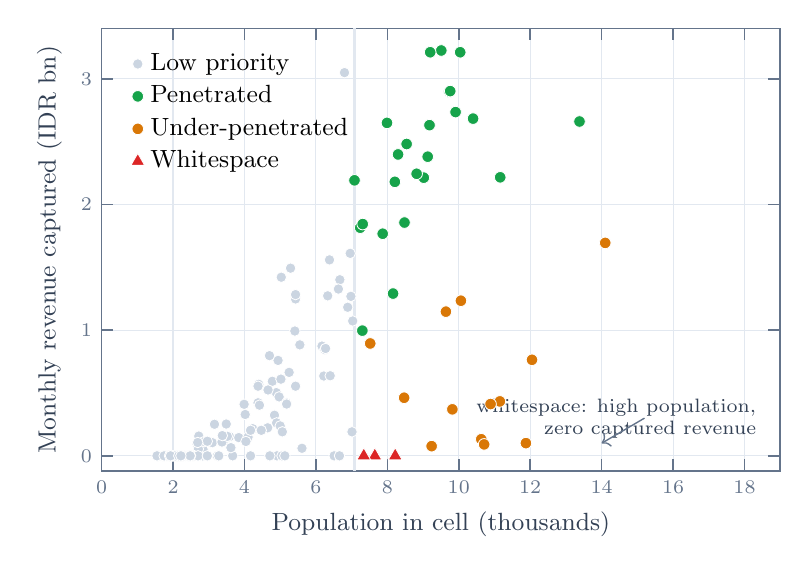
\begin{tikzpicture}
\begin{axis}[
  width=10.2cm, height=7.2cm,
  xlabel={Population in cell (thousands)},
  ylabel={Monthly revenue captured (IDR bn)},
  xmin=0, xmax=19, ymin=-0.12, ymax=3.4,
  axis line style={base}, tick style={base},
  xlabel style={font=\small, text=inkS}, ylabel style={font=\small, text=inkS},
  ticklabel style={font=\scriptsize, text=inkM},
  grid=major, grid style={gridc},
  legend style={draw=none, fill=none, font=\small, at={(0.03,0.97)}, anchor=north west},
  legend cell align=left,
]
\addplot[gridc, line width=0.9pt, forget plot] coordinates {(7.08,-0.12) (7.08,3.4)};
\addplot[only marks, mark=*, mark size=1.9pt, clsLow, mark options={draw=white, line width=0.3pt}] coordinates {(1.86,0.000) (2.07,0.000) (1.59,0.000) (1.76,0.000) (1.91,0.000) (2.21,0.000) (1.89,0.000) (2.48,0.000) (2.48,0.000) (2.83,0.000) (4.23,0.216) (4.78,0.593) (4.40,0.569) (4.94,0.759) (4.02,0.329) (3.58,0.153) (2.68,0.090) (2.43,0.000) (1.96,0.000) (2.04,0.000) (2.12,0.000) (2.25,0.000) (1.56,0.000) (2.27,0.000) (1.75,0.000) (2.12,0.000) (2.34,0.000) (2.42,0.000) (2.75,0.056) (4.84,0.323) (4.70,0.797) (6.17,0.873) (4.89,0.503) (3.41,0.115) (2.47,0.000) (1.81,0.000) (1.83,0.000) (1.97,0.000) (2.10,0.000) (2.02,0.000) (1.71,0.000) (2.57,0.000) (2.30,0.000) (3.28,0.000) (3.84,0.145) (4.65,0.223) (4.97,0.469) (6.96,1.611) (5.43,1.248) (3.99,0.410) (3.10,0.105) (2.12,0.000) (1.57,0.000) (1.55,0.000) (1.75,0.000) (2.06,0.000) (2.17,0.000) (2.19,0.000) (2.84,0.051) (4.47,0.203) (4.66,0.524) (6.25,0.845) (6.33,1.273) (4.38,0.422) (3.37,0.110) (2.10,0.000) (2.12,0.000) (2.14,0.000) (2.17,0.000) (2.27,0.000) (2.21,0.000) (2.71,0.054) (4.90,0.262) (5.18,0.420) (7.03,1.073) (5.02,0.610) (4.10,0.149) (2.60,0.000) (2.30,0.000) (2.23,0.000) (2.54,0.000) (2.16,0.000) (2.72,0.157) (4.42,0.403) (6.98,1.269) (5.61,0.060) (3.67,0.000) (2.70,0.000) (2.23,0.000) (1.93,0.000) (3.62,0.065) (5.18,0.412) (5.41,0.993) (7.01,0.191) (4.71,0.000) (3.24,0.000) (1.98,0.000) (2.49,0.000) (3.16,0.251) (5.43,1.283) (6.51,0.000) (4.91,0.000) (2.06,0.000) (2.96,0.000) (3.49,0.253) (6.67,1.401) (2.48,0.000) (2.87,0.113) (4.38,0.554) (5.29,1.493) (6.80,3.049) (6.63,1.327) (6.89,1.182) (1.90,0.000) (1.93,0.000) (2.96,0.116) (5.25,0.664) (5.03,1.421) (6.38,1.559) (6.27,0.854) (6.22,0.635) (6.40,0.637) (5.43,0.554) (5.55,0.883) (6.66,0.000) (4.71,0.000) (2.16,0.000) (2.22,0.000) (2.69,0.106) (3.52,0.155) (4.04,0.114) (4.17,0.203) (3.38,0.161) (5.00,0.238) (5.06,0.191) (5.05,0.000) (5.13,0.000) (4.17,0.000) (3.28,0.000)};
\addlegendentry{Low priority}
\addplot[only marks, mark=*, mark size=2.1pt, clsPen, mark options={draw=white, line width=0.3pt}] coordinates {(8.21,2.180) (8.30,2.398) (7.24,1.815) (10.16,3.901) (9.40,4.226) (10.83,4.966) (9.51,3.225) (7.87,1.767) (12.06,4.889) (14.95,9.325) (13.82,9.320) (13.25,6.409) (9.20,3.211) (9.02,2.213) (8.54,2.481) (12.05,4.785) (15.01,10.226) (18.03,14.455) (15.13,10.576) (12.76,6.793) (9.18,2.631) (7.31,1.844) (7.99,2.649) (11.86,4.116) (13.14,5.417) (15.26,9.145) (14.32,11.982) (20.53,18.551) (19.36,14.619) (15.28,5.849) (11.16,2.216) (8.82,2.244) (11.44,4.247) (10.27,3.693) (10.88,4.228) (13.95,5.259) (13.57,6.144) (18.93,12.861) (23.42,20.728) (16.55,14.934) (18.89,10.957) (11.67,3.703) (9.40,3.799) (9.84,4.934) (10.17,4.435) (9.80,4.071) (12.14,4.691) (10.30,4.157) (11.92,5.705) (16.08,9.906) (22.47,18.367) (18.36,13.839) (13.44,6.279) (13.38,2.660) (11.07,4.564) (12.67,6.757) (13.88,7.269) (11.48,5.142) (11.99,4.078) (9.74,2.897) (10.04,3.211) (13.67,4.941) (16.92,9.483) (17.32,10.757) (16.98,8.536) (12.40,3.436) (10.42,5.024) (11.30,3.808) (9.13,2.380) (8.48,1.856) (10.40,2.683) (9.76,2.902) (11.90,4.473) (9.91,2.735) (7.08,2.192) (7.30,0.996) (8.16,1.291)};
\addlegendentry{Penetrated}
\addplot[only marks, mark=*, mark size=2.1pt, clsUnd, mark options={draw=white, line width=0.3pt}] coordinates {(8.47,0.462) (10.06,1.234) (12.05,0.764) (10.63,0.132) (14.10,1.694) (11.15,0.433) (10.71,0.091) (9.64,1.147) (10.89,0.412) (11.88,0.101) (7.52,0.894) (9.82,0.370) (9.24,0.077)};
\addlegendentry{Under-penetrated}
\addplot[only marks, mark=triangle*, mark size=2.9pt, clsWhi, mark options={draw=white, line width=0.3pt}] coordinates {(7.65,0.000) (8.22,0.000) (7.34,0.000)};
\addlegendentry{Whitespace}
\node[font=\scriptsize, text=inkS, anchor=south east, align=right] at (axis cs:18.6,0.06)
  {whitespace: high population,\\ zero captured revenue};
\draw[->, inkM, line width=0.5pt] (axis cs:15.2,0.30) -- (axis cs:14.0,0.10);
\end{axis}
\end{tikzpicture}
}
  \caption{Population versus captured revenue per cell, colored by
    classification; whitespace cells sit on the zero-revenue axis at high
    population.}
  \label{fig:scatter}
\end{figure}

% ============================================================================
\section{Targeting Efficiency and Field Applications}
\label{sec:applications}

\subsection{The Price of District-Sized Blocks}

The gain curves of Figure~\ref{fig:gain} quantify what administrative
targeting costs. Ranking resolution-8 cells by density, 50\% of corridor
population is reached within 25.4\% of the land area (43\,km$^2$);
accumulating whole districts requires 38.4\% (66\,km$^2$) for the same
reach. At the 75\% reach level the gap persists: 47.0\% of area
(80\,km$^2$) for hexagons versus 57.8\% (99\,km$^2$) for districts
(Figure~\ref{fig:bars}). Every campaign whose cost scales with area ---
geofenced digital media, leaflet drops, field sampling, canvassing
coverage --- runs ${\sim}$1.2--1.5$\times$ leaner on the spine, and the
advantage widens with the size disparity of the underlying districts,
which on the real archipelago is far larger than in this stylized
corridor.

\subsection{Retail Footprint}

The classification map is the expansion agenda: whitespace cells are
site-selection candidates, scored by $P_h$ and validated in the field.
Before committing a site, Eq.~\eqref{eq:cannibal} prices its interaction
with the existing network --- in the stylized configuration of
Figure~\ref{fig:kring}, two stores four cells (${\sim}3.7$\,km) apart at
$k \le 2$ share a single cell, roughly 5\% of each catchment, a
comfortable spacing; candidate sites closer to existing stores see
$\chi$ rise steeply. The same join against an indexed competitor registry
yields competitor-density covariates for revenue modeling.

\subsection{Network Logistics}

Distribution-center fulfillment zones are $k$-ring (or isochrone-refined)
cell sets with known population, order mass, and revenue --- so an SLA
commitment is a measurable statement about a specific set of hexagons
rather than an aspiration about a \emph{kecamatan}. Daily delivery
manifests group naturally by cell for route assignment, and demand
staging by SKU follows the per-cell order history. The handoff to fleet
optimization is direct: the spine's demand masses $W_h$ are exactly the
gravitational masses consumed by the routing engine
of~\cite{terra2026}.

\subsection{Dynamic Resource Allocation}

Because spine metrics refresh as materialized views, the same machinery
serves operational tempo: field-service and hypercare technicians
assigned to cell clusters during go-lives, and supply--demand imbalances
(transport availability versus order volume per cell) triggering surge
responses in near real time. The unit of allocation is always the same
auditable object --- an H3 cell --- from strategy deck to dispatch board.

\begin{figure}[t]
  \centering
  \resizebox{\columnwidth}{!}{% Auto-generated by generate_figures.py -- do not edit by hand
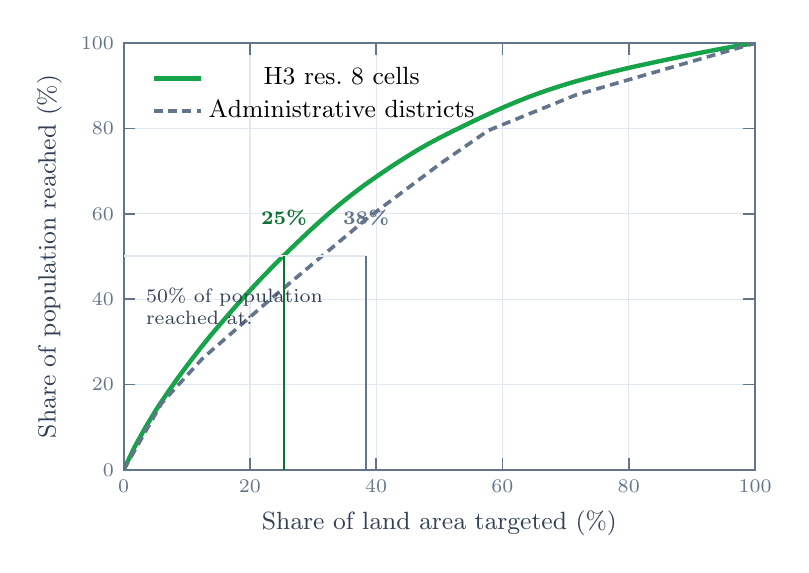
\begin{tikzpicture}
\begin{axis}[
  width=9.6cm, height=7.0cm,
  xlabel={Share of land area targeted (\%)},
  ylabel={Share of population reached (\%)},
  xmin=0, xmax=100, ymin=0, ymax=100,
  axis line style={base}, tick style={base},
  xlabel style={font=\small, text=inkS}, ylabel style={font=\small, text=inkS},
  ticklabel style={font=\scriptsize, text=inkM},
  grid=major, grid style={gridc},
  legend style={draw=none, fill=none, font=\small, at={(0.03,0.97)}, anchor=north west},
]
\addplot[clsPen, line width=1.6pt] coordinates {(0.00,0.00) (1.72,5.32) (3.45,9.93) (5.17,14.14) (6.90,17.97) (8.62,21.60) (10.34,25.03) (12.07,28.36) (13.79,31.52) (15.52,34.52) (17.24,37.48) (18.97,40.36) (20.69,43.14) (22.41,45.83) (24.14,48.42) (25.86,50.94) (27.59,53.40) (29.31,55.82) (31.03,58.15) (32.76,60.42) (34.48,62.55) (36.21,64.59) (37.93,66.52) (39.66,68.33) (41.38,70.07) (43.10,71.77) (44.83,73.39) (46.55,74.96) (48.28,76.42) (50.00,77.77) (51.72,79.07) (53.45,80.32) (55.17,81.56) (56.90,82.77) (58.62,83.95) (60.34,85.08) (62.07,86.16) (63.79,87.18) (65.52,88.14) (67.24,89.02) (68.97,89.86) (70.69,90.65) (72.41,91.37) (74.14,92.06) (75.86,92.72) (77.59,93.35) (79.31,93.96) (81.03,94.54) (82.76,95.10) (84.48,95.65) (86.21,96.19) (87.93,96.72) (89.66,97.24) (91.38,97.75) (93.10,98.24) (94.83,98.72) (96.55,99.18) (98.28,99.61) (100.00,100.00)};
\addlegendentry{H3 res.\ 8 cells}
\addplot[inkM, line width=1.3pt, dash pattern=on 3.2pt off 2pt] coordinates {(0.00,0.00) (6.03,15.63) (12.50,26.11) (23.28,40.01) (38.36,58.68) (50.43,72.05) (57.76,79.54) (71.55,87.81) (100.00,100.00)};
\addlegendentry{Administrative districts}
\addplot[gridc, line width=0.7pt, forget plot] coordinates {(0,50) (38.4,50)};
\addplot[clsPen!70!black, line width=0.7pt, forget plot] coordinates {(25.4,0) (25.4,50)};
\addplot[inkM, line width=0.7pt, forget plot] coordinates {(38.4,0) (38.4,50)};
\node[font=\scriptsize\bfseries, text=clsPen!70!black, anchor=south] at
  (axis cs:25.4,55) {25\%};
\node[font=\scriptsize\bfseries, text=inkM, anchor=south] at
  (axis cs:38.4,55) {38\%};
\node[font=\scriptsize, text=inkS, anchor=north west, align=left] at
  (axis cs:2,45) {50\% of population\\ reached at:};
\end{axis}
\end{tikzpicture}
}
  \caption{Population-reach gain curves: share of corridor population
    reached as a function of land area targeted, cell-by-cell on H3 versus
    whole administrative districts.}
  \label{fig:gain}
\end{figure}

\begin{figure}[t]
  \centering
  \resizebox{0.94\columnwidth}{!}{% Auto-generated by generate_figures.py -- do not edit by hand
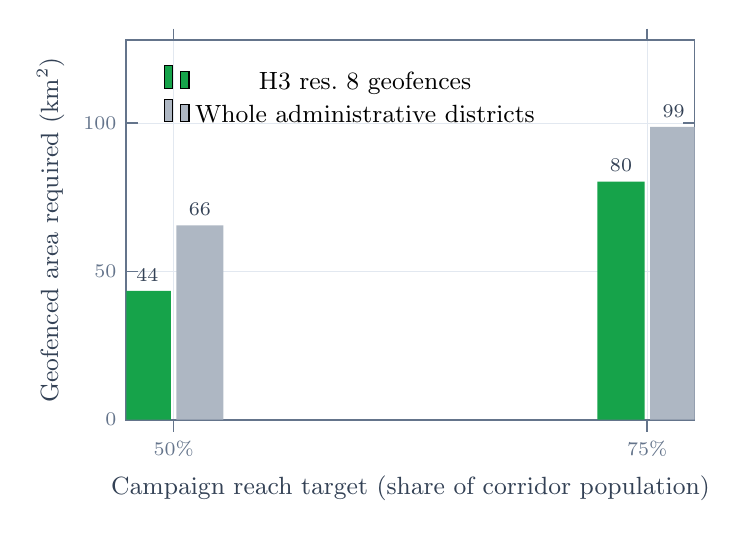
\begin{tikzpicture}
\begin{axis}[
  width=8.8cm, height=6.4cm,
  ybar, bar width=17pt,
  xlabel={Campaign reach target (share of corridor population)},
  ylabel={Geofenced area required (km$^2$)},
  symbolic x coords={50\%, 75\%}, xtick=data,
  ymin=0, ymax=128,
  axis line style={base}, tick style={base},
  xlabel style={font=\small, text=inkS}, ylabel style={font=\small, text=inkS},
  ticklabel style={font=\scriptsize, text=inkM},
  grid=major, grid style={gridc},
  legend style={draw=none, fill=none, font=\small, at={(0.05,0.95)}, anchor=north west},
  nodes near coords, every node near coord/.append style={font=\scriptsize, text=inkS},
  nodes near coords={\pgfmathprintnumber[fixed, precision=0]{\pgfplotspointmeta}},
]
\addplot[fill=clsPen, draw=none] coordinates {(50\%,43.5) (75\%,80.3)};
\addlegendentry{H3 res.\ 8 geofences}
\addplot[fill=inkM!52!white, draw=none] coordinates {(50\%,65.6) (75\%,98.8)};
\addlegendentry{Whole administrative districts}
\end{axis}
\end{tikzpicture}
}
  \caption{Geofenced area required to reach 50\% and 75\% of corridor
    population under hexagon-level versus district-level targeting.}
  \label{fig:bars}
\end{figure}

% ============================================================================
\section{Implementation Roadmap}
\label{sec:roadmap}

The spine earns trust incrementally; each phase ships a usable artifact.

\textbf{Phase 1 --- Proof of concept (one region, one KPI).} Build the
spine for a single high-density region (Greater Jakarta), join internal
store revenue against open population data~\cite{kontur} at resolution~8,
and publish one governed metric --- revenue per capita per cell --- with
the classification map of Eq.~\eqref{eq:class}. Everything in
Section~\ref{sec:casestudy} is achievable in this phase with no new
infrastructure; the deliverable is the whitespace shortlist and the
stakeholder conversation it starts.

\textbf{Phase 2 --- Pipeline automation.} Move indexing to ingestion:
nightly batch transforms convert raw POS/ERP coordinates into H3 strings
inside the warehouse, the spine dimension and metric marts become
scheduled materialized views, and the classification thresholds
$(P^{*}, r^{*})$ move from notebook constants to versioned configuration.
Data-quality gates (geocode validity, coordinate-swap detection,
cell-coverage drift) are attached to the load, because from this phase on
the spine is load-bearing.

\textbf{Phase 3 --- National scale and advanced primitives.} Extend the
spine across the operating territory, activate $k$-ring analytics
(cannibalization screens, DC fulfillment zones), calibrate the decay
length $\tau$ and store attractiveness $a_s$ per format from delivery and
loyalty data, and connect downstream consumers --- media geofencing
exports, dispatch clustering, and the routing engine
of~\cite{terra2026}. Regional divergence matters at this stage: dense
Java corridors and sparse eastern territories warrant different working
resolutions, selected per region exactly as the companion framework
selects routing parameters.

% ============================================================================
\section{Limitations and Future Work}
\label{sec:limitations}

\textbf{Synthetic calibration.} The corridor is a stylized artifact:
magnitudes (ARPU, opportunity sizing) illustrate the workflow, not the
market. The immediate next step is re-running the identical SQL against
production POS data and Kontur population --- the figures regenerate
unchanged because they consume only the spine schema.

\textbf{Grid-distance decay.} Eq.~\eqref{eq:capture} decays with hex-grid
distance, which ignores rivers, toll barriers, and one-way systems.
Isochrone-refined kernels (travel-time bands from the routing stack) are
a drop-in replacement where site decisions are close.

\textbf{Ecological inference.} Cell-level correlation is not
customer-level behavior; resolution-8 aggregates ${\sim}$thousands of
residents, and inferences about individuals from cell metrics commit the
ecological fallacy. The spine bounds, it does not replace,
customer-level analytics.

\textbf{Boundary effects at coarse rollups.} Aperture-7 parentage is
approximate at cell edges; metrics rolled up several resolutions can
shift small mass between parents. For executive rollups this is
immaterial; for contractual SLA geometry, compute at the working
resolution.

\textbf{Threshold sensitivity.} The four-class taxonomy inherits the
percentile choices $(P^{*}, r^{*})$; a sensitivity sweep belongs in the
Phase-2 automation so that the whitespace list ships with its stability
band.

% ============================================================================
\section{Conclusion}
\label{sec:conclusion}

Strategic market analysis fails quietly when its spatial unit is wrong:
district choropleths that hide urban demand, catchments amputated at
provincial borders, and histories severed by \emph{pemekaran} are not
data problems but geometry problems. The H3 Spine fixes the geometry
once, at ingestion, and lets everything downstream --- population joins,
revenue capture, penetration classification, cannibalization screens,
targeting gain curves --- run as ordinary SQL on one shared key. On a
reproducible Jakarta--Tangerang corridor the approach rediscovered a
deliberately planted market gap, priced it at ${\sim}$IDR~8.4\,bn per
month, and cut the area cost of reaching half the population by a third
relative to district targeting. The same cells then feed routing,
dispatch, and geofencing without translation. Hexagons are not the
insight; the discipline of one fixed, uniform, hierarchical spatial key
under every layer of the business is --- and the corridor study shows it
can be stood up with open data and a weekend of SQL.

% ============================================================================
\begin{thebibliography}{9}
\small

\bibitem{brodsky2018}
I.~Brodsky,
``H3: Uber's Hexagonal Hierarchical Spatial Index,''
Uber Engineering Blog, 2018.
[Online]. Available: \url{https://www.uber.com/blog/h3/}

\bibitem{h3docs}
Uber Technologies,
\emph{H3 Documentation: Tables of Cell Statistics Across Resolutions}.
[Online]. Available: \url{https://h3geo.org/docs/core-library/restable/}

\bibitem{crawford2023}
M.~Crawford,
``Use H3 to Create Multiresolution Hexagon Grids in ArcGIS Pro 3.1,''
Esri ArcGIS Blog, 2023.
[Online]. Available:
\url{https://www.esri.com/arcgis-blog/products/arcgis-pro/analytics/use-h3-to-create-multiresolution-hexagon-grids-in-arcgis-pro-3-1}

\bibitem{esriwhyhex}
Esri,
\emph{Why Hexagons? ArcGIS Pro Tool Reference}.
[Online]. Available:
\url{https://pro.arcgis.com/en/pro-app/latest/tool-reference/spatial-statistics/h-whyhexagons.htm}

\bibitem{openshaw1984}
S.~Openshaw,
\emph{The Modifiable Areal Unit Problem}, ser.\ CATMOG no.~38.
Norwich, UK: Geo Books, 1984.

\bibitem{reilly1931}
W.~J. Reilly,
\emph{The Law of Retail Gravitation}.
New York, NY: Knickerbocker Press, 1931.

\bibitem{huff1964}
D.~L. Huff,
``Defining and Estimating a Trading Area,''
\emph{Journal of Marketing}, vol.~28, no.~3, pp.~34--38, 1964.

\bibitem{zipf1946}
G.~K. Zipf,
``The $P_1 P_2 / D$ Hypothesis: On the Intercity Movement of Persons,''
\emph{American Sociological Review}, vol.~11, no.~6, pp.~677--686, 1946.

\bibitem{kontur}
Kontur Inc.,
\emph{Kontur Population: Global Population Density for 400\,m H3 Hexagons}.
[Online]. Available: \url{https://data.humdata.org/dataset/kontur-population-dataset}

\bibitem{snowflakeh3}
Snowflake Inc.,
\emph{H3 Geospatial Functions --- Snowflake Documentation}.
[Online]. Available:
\url{https://docs.snowflake.com/en/sql-reference/functions-geospatial}

\bibitem{bigqueryjslibs}
CARTO,
\emph{Analytics Toolbox for BigQuery: H3 Module}.
[Online]. Available: \url{https://docs.carto.com/analytics-toolbox-bigquery}

\bibitem{terra2026}
A.~Dobson,
``When a Jakarta Kilometer Isn't an Ambon Kilometer: Context-Aware Fleet
Routing Across Indonesia's Asymmetric Geographies,''
IT Paragon Enterprise Logistics Research, working paper, 2026.

\bibitem{haklay2008}
M.~Haklay and P.~Weber,
``OpenStreetMap: User-Generated Street Maps,''
\emph{IEEE Pervasive Computing}, vol.~7, no.~4, pp.~12--18, 2008.

\end{thebibliography}

\end{document}
